\documentclass[11pt,a4paper]{article}
\usepackage[utf8]{inputenc}
\usepackage[T1]{fontenc}
\usepackage[spanish,es-noshorthands]{babel}
\usepackage{geometry}
\geometry{margin=2.6cm}
\usepackage{calc}
\usepackage{longtable}
\usepackage{booktabs}
\usepackage{array}
\usepackage{ragged2e}
\usepackage{graphicx}
\usepackage{float}
\usepackage[table]{xcolor}
\usepackage{caption}
\captionsetup{skip=6pt}
\usepackage{titlesec}
\usepackage{fancyhdr}
\usepackage[hidelinks]{hyperref}
\usepackage{enumitem}
\usepackage{parskip}
\usepackage{needspace}
\usepackage{etoolbox}
\setlength{\parskip}{0.55em}
\setlist{itemsep=0.2em}

% evita titulos "huerfanos" solos al final de una pagina, empujandolos a la
% siguiente si no queda espacio para el titulo mas unas lineas de contenido
\pretocmd{\section}{\needspace{5\baselineskip}}{}{}
\pretocmd{\subsection}{\needspace{4\baselineskip}}{}{}
\pretocmd{\subsubsection}{\needspace{3\baselineskip}}{}{}

% --- Macros pandoc espera que existan (normalmente las inyecta su modo -s) ---
\providecommand{\tightlist}{%
  \setlength{\itemsep}{0pt}\setlength{\parskip}{0pt}}
\providecommand{\pandocbounded}[1]{#1}
\newcommand{\passthrough}[1]{#1}

\hypersetup{
  pdftitle={HemoScan Andino},
  pdfauthor={Equipo HemoScan Andino -- UPeU Juliaca},
  colorlinks=false,
  bookmarksopen=true
}

% El contenido ya trae su propia numeracion manual (1., 1.1, 1.1.1...) escrita
% en el texto de cada encabezado, asi que se desactiva la numeracion automatica
% de LaTeX para evitar una doble numeracion en el indice y en el cuerpo.
\setcounter{secnumdepth}{-2}
\setcounter{tocdepth}{4}
\titleformat{\section}{\normalfont\Large\bfseries}{}{0em}{}
\titleformat{\subsection}{\normalfont\large\bfseries}{}{0em}{}
\titleformat{\subsubsection}{\normalfont\normalsize\bfseries}{}{0em}{}

% Encabezado con dos etiquetas CORTAS y de ancho fijo (nunca texto largo o
% dinamico por subseccion) para que jamas puedan solaparse entre si.
\pagestyle{fancy}
\fancyhf{}
\fancyhead[L]{\small HemoScan Andino}
\fancyhead[R]{\small Software E2 --- Datos}
\fancyfoot[C]{\thepage}
\renewcommand{\headrulewidth}{0.4pt}

\begin{document}

\begin{titlepage}
\centering
\vspace*{1.2cm}
{\large UNIVERSIDAD PERUANA UNI\'ON\par}
{\normalsize Facultad de Ingenier\'ia y Arquitectura\par}
{\normalsize Escuela Profesional de Ingenier\'ia de Sistemas --- Filial Juliaca\par}
\vspace{0.5cm}
\rule{0.6\linewidth}{0.4pt}
\vspace{1.6cm}

{\large PROYECTO DE TESIS / PROYECTO INTEGRADOR\par}
\vspace{1.0cm}
{\huge\bfseries HemoScan Andino\par}
\vspace{0.6cm}
{\Large Sistema no invasivo de tamizaje de anemia infantil con fusi\'on \'optica multisensor y autocalibraci\'on por altitud\par}
\vspace{1.6cm}
\rule{0.6\linewidth}{0.4pt}
\vspace{1.6cm}

{\Large\bfseries Entregable 2 de Software (CE022, Parte 1) --- Plataforma de Datos del Sistema\par}
\vspace{2.0cm}

{\normalsize Juliaca, Puno, Per\'u \par}
{\normalsize Julio de 2026\par}

\vfill
\end{titlepage}

\tableofcontents
\newpage

\textbf{Entregable N.° 6 --- Plataforma de Datos del Sistema}
\#\#\# Parte 1 (Semestre 1): Modelo de Datos e Implementación de Base de Datos

\emph{(Sexto entregable consecutivo del proyecto HemoScan Andino. Corresponde al Entregable N.° 2 de la competencia CE022 --- Área C: Ingeniería de Software; utiliza una numeración de Entregable propia y distinta de la de los Entregables N.° 1-4 del Área B --- Gestión de TI --- y N.° 5 del Área C --- Ingeniería de Software --- ya presentados, aunque continúa la secuencia documental global del proyecto. Tal como lo anticipó explícitamente el Entregable N.° 7 --- Diseño de Red, Área A --- Infraestructura Tecnológica {[}``El número 6 se reserva a un entregable en elaboración paralela de otra área de competencia del mismo proyecto, no desarrollado en este documento''{]}, este es precisamente ese entregable.)}

\textbf{Área de competencia:} Área C --- Ingeniería de Software
\textbf{Competencia:} CE022 --- Ingeniería de la Información
\textbf{Evidencia que cubre este documento (Parte 1 de 2):} CE0221 (Modelo de datos relacional documentado y validado) y CE0222 (Base de datos relacional implementada y consultable). Las evidencias CE0223 (motor transaccional y procedimientos avanzados) y CE0224 (administración y seguridad de base de datos empresarial) corresponden a la \textbf{Parte 2}, de desarrollo previsto en el Semestre 2 (ver Secciones 3 y 4).
\textbf{Paquete de la Estructura de Desglose del Trabajo (EDT) que satisface:} 4.2 --- ``Modelo de datos y mapeo FHIR'' (Entregable N.° 3, sección 3.2.3), responsable Integrante 3, cuyo criterio de aceptación formal es \emph{``cada campo clínico mapeado a un recurso/atributo FHIR --- atiende A5, A14 (Entregable N.° 4)''}. Se distingue explícitamente del paquete EDT 2.2 --- ``Servidor/nube y base de datos'' (Integrante 1, Entregable N.° 3), responsable del aprovisionamiento del \textbf{servidor físico/nube real} de la posta donde este modelo se desplegará en producción: este documento diseña e implementa (en un entorno de validación) el esquema; el paquete 2.2 aprovisiona el motor donde ese esquema correrá en Fase 0 real.
\textbf{Sistema documentado:} HemoScan Andino --- capa de datos relacional (PostgreSQL 16 + PostGIS 3.4) que sustenta el backend de interoperabilidad FHIR (FastAPI/NestJS), la aplicación móvil Flutter/PWA offline-first y la plataforma web de analítica geoespacial (React/TypeScript)

\textbf{Organización diagnosticada (caso ilustrativo y representativo):} Microred de Salud Altiplano-Puno

\begin{center}\rule{0.5\linewidth}{0.5pt}\end{center}

\textbf{Integrantes del equipo:}

{\small
\begin{longtable}[]{@{}
  >{\raggedright\arraybackslash}p{(\linewidth - 4\tabcolsep) * \real{0.3333}}
  >{\raggedright\arraybackslash}p{(\linewidth - 4\tabcolsep) * \real{0.3333}}
  >{\raggedright\arraybackslash}p{(\linewidth - 4\tabcolsep) * \real{0.3333}}@{}}
\toprule\noalign{}
\begin{minipage}[b]{\linewidth}\raggedright
N.°
\end{minipage} & \begin{minipage}[b]{\linewidth}\raggedright
Integrante
\end{minipage} & \begin{minipage}[b]{\linewidth}\raggedright
Rol / Área de competencia
\end{minipage} \\
\midrule\noalign{}
\endhead
\bottomrule\noalign{}
\endlastfoot
1 & \textit{(Integrante 1, Líder de Infraestructura Tecnológica -- nombre por completar)} & CE03 --- Infraestructura Tecnológica (red, seguridad, centro de datos) \\
2 & \textit{(Integrante 2, Líder de Gestión de TI -- nombre por completar)} & CE01 --- Gestión de TI (diagnóstico, business case, plan de gestión, procesos) \\
3 & \textit{(Integrante 3, Líder de Ingeniería de Software -- nombre por completar)} & CE02 --- Ingeniería de Software (requerimientos, datos, sistema, calidad) --- \textbf{responsable principal de este entregable} \\
\end{longtable}
}

\textbf{Docente asesor(a) del curso:} \textit{(nombre del docente asesor por completar)}
\textbf{Curso / Sílabo:} \textit{(nombre del curso / s\'ilabo por completar)}
\textbf{Ciclo académico:} 2026-I (supuesto, a confirmar con la programación académica vigente)

\textbf{Lugar y fecha:} Juliaca, Puno, Perú --- 07 de julio de 2026

\begin{center}\rule{0.5\linewidth}{0.5pt}\end{center}

\begin{quote}
\textbf{Nota metodológica y alcance (léase antes de continuar).} Este documento es el Entregable N.° 6 del proyecto HemoScan Andino, competencia \textbf{CE022 --- Ingeniería de la Información}, y desarrolla \textbf{únicamente la Parte 1} del producto exigido por su rúbrica: la Sección 1 (Modelo de Datos) y la Sección 2 (Implementación de Base de Datos) se desarrollan en profundidad; las Secciones 3 (Consultas y Programación en Base de Datos) y 4 (Seguridad y Administración) se dejan como \textbf{placeholders de alcance explícito para una Parte 2, de desarrollo previsto en el Semestre 2}, siguiendo instrucción directa del encargo de este entregable. Se declaran seis límites de honestidad técnica y decisiones metodológicas, en la misma disciplina de transparencia ya sostenida en los cinco entregables anteriores del proyecto:

\textbf{Primero}, este modelo de datos \textbf{toma como insumo fijo y no reinterpretable} los identificadores, el diagrama de clases (Diagrama 6) y el mapeo a los seis recursos FHIR (sección 4.5) ya establecidos en el \textbf{Entregable N.° 5} (Requerimientos y Diseño del Sistema): las 40 RF, 20 RNF, 12 RN, 11 CU y 10 ADR allí fijados se citan tal cual, sin renumerar. La sección 1.4 de este documento hace explícita, entidad por entidad, la trazabilidad y las diferencias de traducción entre aquel diagrama de clases (orientado a objetos de software) y este modelo relacional (orientado a persistencia normalizada).

\textbf{Segundo}, y de forma específica para este entregable, se incorporan \textbf{tres entidades nuevas} no presentes como clases en el Diagrama 6 del Entregable N.° 5 (\texttt{agente\_comunitario}, la tabla técnica \texttt{recurso\_fhir} y la tabla de unión \texttt{paciente\_cuidador}), exigidas por el alcance explícito de la competencia CE022 (``entidades de gestión: usuarios/roles, microredes, agentes comunitarios'') o por necesidades de normalización relacional que no existen a nivel de un diagrama de clases de software. Cada una se documenta explícitamente como una \textbf{extensión, nunca una contradicción}, del modelo previo. De igual manera, la entidad \texttt{establecimiento\_salud} (equivalente funcional a un recurso FHIR \emph{Location}) se incorpora como tabla de apoyo geoespacial-administrativo; \textbf{no} se cuenta como un séptimo recurso FHIR clínico y \textbf{no} contradice el ADR-06 del Entregable N.° 5 (que fijó el alcance en 6 recursos clínicos para Fase 0) --- la aclaración completa se desarrolla en la sección 1.4.

\textbf{Tercero}, todos los valores clínicos exactos que dependen del texto íntegro de la \textbf{NTS 213-MINSA/DGIESP-2024} (puntos de corte de hemoglobina, fórmula exacta de corrección por altitud, posología de hierro) permanecen \textbf{{[}DATO PENDIENTE DE VALIDAR{]}}, tal como ya se declaró en los Entregables N.° 4 y N.° 5; el modelo de datos se diseña deliberadamente para parametrizar y versionar estos valores (tabla \texttt{config.configuracion\_clinica}, JSONB versionado) en lugar de fijarlos, materializando la regla de negocio RN-02.

\textbf{Cuarto}, y en un esfuerzo deliberado por superar la limitación de ``diseño no ejecutado'' señalada como pendiente en entregables previos, \textbf{los scripts DDL y DML de este documento se ejecutaron realmente} contra una instancia efímera de PostgreSQL 16.4 + PostGIS 3.4.3, desplegada en un contenedor Docker local (imagen \texttt{postgis/postgis:16-3.4}, digest inmutable \texttt{sha256:44126d872ac91993766c341e369c539e8196614321765d36a6f1bab0419a5fa5}) únicamente para fines de validación de este entregable, el 2026-07-07. A diferencia de las cinco entregas anteriores del proyecto, esta afirmación \textbf{no depende únicamente de la palabra de este documento}: los cuatro scripts (DDL, DML, consultas de verificación y pruebas de integridad), el \texttt{docker-compose.yml} exacto usado y las transcripciones crudas y sin editar de cada corrida quedan archivados como \textbf{archivos separados, verificables de forma independiente por checksum SHA-256}, en la carpeta hermana \texttt{Anexos-Ejecutables-Entregable-06/} (ver su \texttt{README.md} para el detalle de checksums, el procedimiento exacto de reproducción y las dos cifras que la propia ejecución real permitió corregir frente a lo que se había narrado). La Sección 2 y los Anexos A a D de este documento resumen y citan esa evidencia; el registro crudo completo vive únicamente en esos archivos externos, no solo como texto narrativo dentro de este Markdown. Se declara con la misma honestidad que \textbf{esta instancia efímera no es, bajo ninguna interpretación, el servidor de producción de la posta}: ese aprovisionamiento sigue siendo responsabilidad del paquete EDT 2.2 del Integrante 1, como ya se aclaró en el encabezado de este documento. El contenedor efímero ya fue destruido tras capturar la evidencia (\texttt{docker\ compose\ down}); lo que persiste y es reproducible en cualquier momento son los scripts, el \texttt{docker-compose.yml} y los logs crudos, no el contenedor en sí.

\textbf{Quinto}, todos los datos cargados mediante el script DML (Sección 2.4, Anexo B) son \textbf{enteramente ficticios e ilustrativos}, generados únicamente para validar que el esquema funciona con datos de forma realista. \textbf{Ningún dato de este documento corresponde a una niña, niño, cuidador/a o profesional de salud real}: no existe todavía convenio institucional con ninguna microred (Nota metodológica del Entregable N.° 5), por lo que ---dada además la máxima sensibilidad de tratarse de datos de salud de menores de edad bajo la Ley N.° 29733--- construir o utilizar un dataset real está fuera de alcance ético y de posibilidad práctica de este entregable.

\textbf{Sexto}, sobre la extensión de este documento frente al límite de 15-25 páginas de la plantilla del producto: esta Parte 1 desarrolla en profundidad únicamente 2 de las 4 secciones exigidas por la rúbrica completa (Modelo de Datos e Implementación de Base de Datos; las Secciones 3 y 4 son \emph{placeholders} de alcance para el Semestre 2), y además incorpora, como evidencia directa de ejecución real, cuatro anexos (A-D) con scripts y salidas de motor que un documento puramente de diseño no necesitaría. Aun así, se reconoce con la misma honestidad de esta nota que el documento, en su versión final, sigue siendo más extenso de lo que ese límite sugiere: se condensaron los Anexos A y B (que antes reproducían íntegros los 429+348 líneas de los scripts DDL y DML dentro del propio Markdown) a un extracto representativo, moviendo el contenido completo y verificable a los archivos externos de \texttt{Anexos-Ejecutables-Entregable-06/}, lo que evita duplicar ese contenido dos veces dentro de este documento y reduce su extensión; no se afirma, sin embargo, que el resultado final quede ya dentro del rango de 15-25 páginas de un producto completo --- eso corresponde evaluarlo formalmente contra la plantilla en la integración final con la Parte 2 (Semestre 2), cuando el documento combinado exista y pueda paginarse como una sola entrega.
\end{quote}

\begin{center}\rule{0.5\linewidth}{0.5pt}\end{center}

\section{Resumen Ejecutivo}\label{resumen-ejecutivo}

Si HemoScan Andino es, en esencia, un sistema que transforma tres señales ópticas de bajo costo en una decisión de salud pública auditable, entonces \textbf{la plataforma de datos es el componente que hace posible que esa transformación sea confiable, trazable y reproducible en el tiempo} --- no un contenedor pasivo de registros, sino el mecanismo que materializa, a nivel de motor de base de datos y no solo de intención de diseño, tres compromisos ya asumidos por el proyecto en entregables anteriores: que ninguna determinación de hemoglobina pierda su cadena de corrección por altitud (RN-02, RN-03), que ninguna captura de datos de un menor de edad ocurra sin un consentimiento vigente verificable (RN-04) y que ningún acceso a datos clínicos quede sin registro auditable (RN-11). Este Entregable N.° 6, competencia \textbf{CE022 --- Ingeniería de la Información}, desarrolla la primera mitad de esa plataforma: el \textbf{modelo de datos} (conceptual, lógico y normalizado, con su diccionario de datos completo) y su \textbf{implementación real} en PostgreSQL 16 con la extensión PostGIS, dejando para una Parte 2 en Semestre 2 la programación avanzada de base de datos (funciones, disparadores, procedimientos almacenados) y la administración de seguridad a nivel de motor (roles de base de datos, cifrado de columna, políticas de auditoría del propio gestor).

El modelo resultante organiza \textbf{24 tablas y 1 vista derivada} en \textbf{cuatro esquemas} que reproducen, a nivel de base de datos, la misma modularidad de dominio ya declarada arquitectónicamente en el ADR-02 del Entregable N.° 5 (monolito modular): \texttt{clinico} (15 tablas alineadas a los recursos FHIR Patient, Consent, Device, Observation, Provenance y AuditEvent), \texttt{geo} (3 tablas geoespaciales sobre PostGIS: microredes, establecimientos de salud con altitud y la capa agregada de hexágonos H3), \texttt{config} (2 tablas de parámetros clínicos versionados, que materializan la regla de negocio RN-02) y \texttt{gestion} (4 tablas de usuarios, roles RBAC, agentes comunitarios de salud y alertas de stock). El diseño resuelve explícitamente dos problemas de modelado no triviales heredados del carácter FHIR del proyecto: la referencia polimórfica del recurso \texttt{AuditEvent} (que en el estándar FHIR puede apuntar a cualquiera de otros cinco tipos de recurso) se resuelve mediante una tabla técnica compartida (\texttt{recurso\_fhir}) que preserva integridad referencial real de PostgreSQL, evitando una clave foránea débil validada solo en aplicación; y la cardinalidad 1:1 de la cadena Captura -\textgreater{} CorrecciónAltitud -\textgreater{} Determinación (ya definida en el Diagrama 6 del Entregable N.° 5) se refuerza en el esquema físico mediante restricciones \texttt{UNIQUE}, en lugar de colapsarse en una única tabla ancha, preservando así a nivel de base de datos el mismo principio de independencia auditable que el ADR-05 exige a nivel de componentes de software.

De manera consistente con la disciplina de honestidad técnica del proyecto, este entregable no se limita a presentar scripts SQL redactados en papel: \textbf{el script DDL completo (24 tablas, 1 vista, 40 restricciones CHECK, 39 llaves foráneas, 14 restricciones UNIQUE y 60 índices) y el script DML de carga inicial se ejecutaron realmente} contra una instancia de PostgreSQL 16.4 con PostGIS 3.4.3 desplegada en un contenedor Docker local, y su salida real ---incluyendo consultas de verificación (uniones múltiples, agregaciones, consultas geoespaciales con \texttt{ST\_Distance} y \texttt{ORDER\ BY\ \textless{}-\textgreater{}}, y una traza de auditoría completa) y siete pruebas deliberadas de violación de restricciones más un control positivo, todas con el resultado correcto--- se documenta en la Sección 2 y en los Anexos A a D. A diferencia de una simple afirmación narrativa, esta ejecución quedó archivada como evidencia externa al propio documento ---cuatro scripts \texttt{.sql}, el \texttt{docker-compose.yml} usado y las transcripciones crudas de cada corrida, todo verificable por checksum SHA-256 en la carpeta \texttt{Anexos-Ejecutables-Entregable-06/}---, de modo que la afirmación ``se ejecutó realmente'' no depende únicamente de la palabra de este Markdown. Esta evidencia de ejecución real e independientemente verificable, y no solo de diseño en papel, es la principal fortaleza que este entregable aporta frente a los cinco documentos anteriores del proyecto, todos ellos ---por diseño y por etapa--- ejercicios de gabinete no ejecutados.

\begin{center}\rule{0.5\linewidth}{0.5pt}\end{center}

\section{1. Modelo de Datos}\label{modelo-de-datos}

\subsection{1.1 Alcance de esta Parte 1 y relación con el Entregable N.° 5}\label{alcance-de-esta-parte-1-y-relaciuxf3n-con-el-entregable-n.-5}

El Entregable N.° 5 ya produjo, en su sección 4.2 (Diagrama 6) y su sección 4.5, un diagrama de clases de 20 entidades y un mapeo detallado a los seis recursos FHIR del proyecto. Ese trabajo fue deliberadamente un ejercicio de \textbf{diseño orientado a objetos de software} (clases, atributos, asociaciones), no un modelo relacional normalizado ni un esquema físico de base de datos: el propio Entregable N.° 5 lo declara así en su alcance (sección 4, ``Diseño Detallado''). La tarea específica de la competencia \textbf{CE022 --- Ingeniería de la Información} es distinta y complementaria: tomar ese diseño como insumo fijo y producir a partir de él (a) un modelo entidad-relación explícito, (b) su forma lógica relacional, (c) la prueba de que dicha forma cumple las reglas de normalización, (d) un diccionario de datos exhaustivo y (e) su implementación real y consultable en un motor de base de datos concreto --- PostgreSQL 16 con la extensión PostGIS, ya fijado como decisión arquitectónica en el ADR-10 del Entregable N.° 5.

Esta Parte 1 cubre íntegramente las evidencias \textbf{CE0221} (modelo de datos relacional documentado y validado) y \textbf{CE0222} (base de datos relacional implementada y consultable). Quedan fuera de alcance de esta Parte 1 --- y se marcan explícitamente como tales en las Secciones 3 y 4 --- las evidencias \textbf{CE0223} (funciones, disparadores y procedimientos almacenados; control transaccional avanzado) y \textbf{CE0224} (roles de base de datos distintos de los de aplicación, cifrado a nivel de columna, políticas de auditoría del motor, replicación y recuperación ante desastres), cuyo desarrollo está previsto para una Parte 2 en el Semestre 2, siguiendo instrucción explícita del encargo de este entregable.

\subsection{1.2 Arquitectura de la información: cuatro dominios y su justificación}\label{arquitectura-de-la-informaciuxf3n-cuatro-dominios-y-su-justificaciuxf3n}

El modelo se organiza en cuatro esquemas (\emph{namespaces} de PostgreSQL) que agrupan las tablas por dominio de responsabilidad, replicando a nivel de base de datos la misma frontera de módulos que el ADR-02 del Entregable N.° 5 ya fijó a nivel de componentes de backend (identidad, clínico/FHIR, geoespacial, etc.), sin que esto implique, en ningún caso, una arquitectura de microservicios ni bases de datos físicamente separadas --- los cuatro esquemas conviven en una única base de datos (\texttt{hemoscan\_andino}), consistente con el ADR-10 (PostgreSQL/PostGIS como único motor).

{\small
\begin{longtable}[]{@{}
  >{\raggedright\arraybackslash}p{(\linewidth - 6\tabcolsep) * \real{0.2500}}
  >{\raggedright\arraybackslash}p{(\linewidth - 6\tabcolsep) * \real{0.2500}}
  >{\raggedright\arraybackslash}p{(\linewidth - 6\tabcolsep) * \real{0.2500}}
  >{\raggedright\arraybackslash}p{(\linewidth - 6\tabcolsep) * \real{0.2500}}@{}}
\toprule\noalign{}
\begin{minipage}[b]{\linewidth}\raggedright
Esquema
\end{minipage} & \begin{minipage}[b]{\linewidth}\raggedright
Propósito
\end{minipage} & \begin{minipage}[b]{\linewidth}\raggedright
N.° de tablas
\end{minipage} & \begin{minipage}[b]{\linewidth}\raggedright
Tablas
\end{minipage} \\
\midrule\noalign{}
\endhead
\bottomrule\noalign{}
\endlastfoot
\texttt{clinico} & Entidades clínicas alineadas a los seis recursos FHIR del proyecto (Patient, Consent, Device, Observation, Provenance, AuditEvent) y sus entidades de apoyo directo & 15 & \texttt{recurso\_fhir}, \texttt{paciente}, \texttt{cuidador}, \texttt{paciente\_cuidador}, \texttt{consentimiento}, \texttt{dispositivo}, \texttt{captura}, \texttt{correccion\_altitud}, \texttt{determinacion}, \texttt{alerta\_derivacion}, \texttt{caso\_confirmacion}, \texttt{prescripcion}, \texttt{provenance}, \texttt{auditevent}, \texttt{control\_mensual} \\
\texttt{geo} & Organización territorial y agregación geoespacial sobre PostGIS & 3 & \texttt{microrred}, \texttt{establecimiento\_salud}, \texttt{hexagono\_cobertura} \\
\texttt{config} & Parámetros clínicos versionados y auditables (materializa RN-02) & 2 & \texttt{modelo\_inferencia}, \texttt{configuracion\_clinica} \\
\texttt{gestion} & Usuarios, roles RBAC, agentes comunitarios de salud y alertas administrativas & 4 & \texttt{rol}, \texttt{usuario\_sistema}, \texttt{agente\_comunitario}, \texttt{alerta\_stock} \\
\end{longtable}
}

\textbf{Convención de nomenclatura.} Todos los identificadores técnicos (esquemas, tablas, columnas, restricciones) se escriben en \texttt{snake\_case}, en español, \textbf{sin tildes ni eñes} (p.~ej. \texttt{senal\_ppg\_ref}, no \texttt{señal\_ppg\_ref}), siguiendo una práctica estándar de portabilidad de bases de datos que evita ambigüedades de codificación de caracteres entre entornos (Windows/Linux, distintas configuraciones de \emph{locale}). Esta convención afecta únicamente a los nombres técnicos internos; los textos visibles al usuario final (interfaz de la app y de la plataforma web) sí conservan la ortografía correcta del español, por no ser competencia de este entregable.

\textbf{Diagrama 1 --- Vista general de la arquitectura de información (cuatro esquemas y sus dependencias).}

\begin{figure}[H]
\centering
\pandocbounded{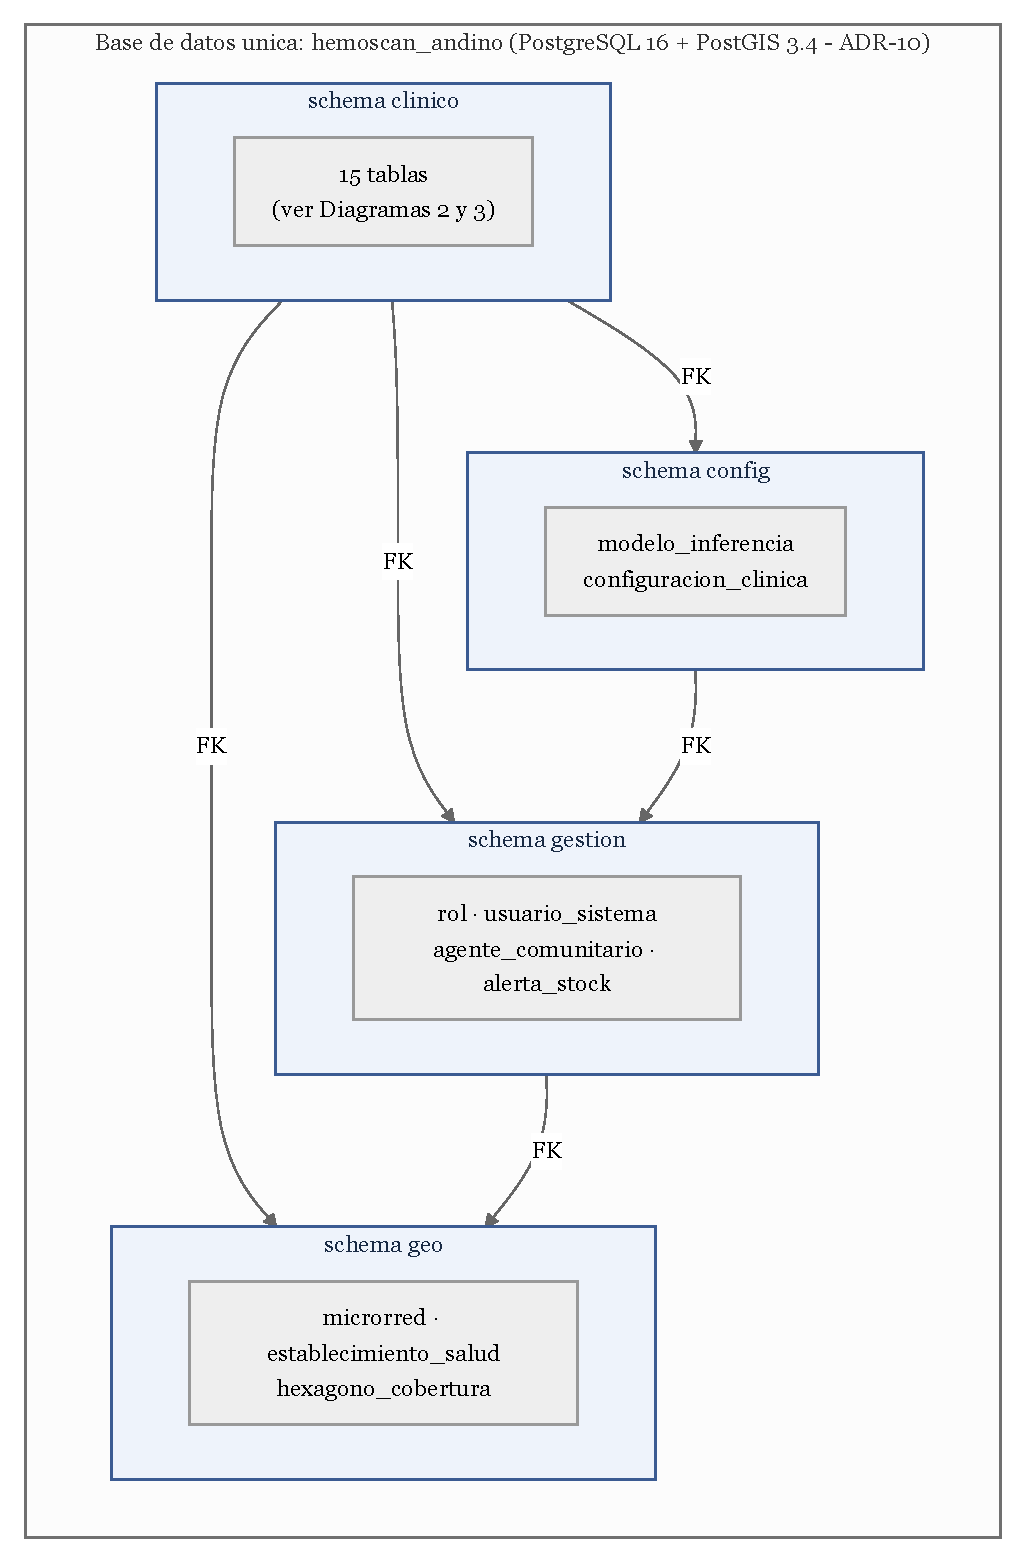
\includegraphics[width=0.85\linewidth,keepaspectratio]{assets/06-plataforma-datos/diagrama-01-arquitectura-esquemas.pdf}}
\end{figure}

\subsection{1.3 Modelo Entidad-Relación (nivel conceptual)}\label{modelo-entidad-relaciuxf3n-nivel-conceptual}

Se presentan cinco diagramas complementarios en notación entidad-relación (\emph{crow's foot}), especificados como diagrama-como-código y renderizados a imagen vectorial con un renderizador libre de licencia (Mermaid); las multiplicidades se leen \texttt{1}, \texttt{0..1}, \texttt{0..*}, \texttt{1..*} sobre cada relación. Por legibilidad, dado que el esquema \texttt{clinico} concentra 15 tablas, se separa su presentación en dos diagramas: el núcleo de la cadena clínica (Diagrama 2) y la resolución de la referencia poli\-mórfica de auditoría (Diagrama 3).

\textbf{Diagrama 2 --- Modelo E-R del núcleo clínico (esquema \texttt{clinico}, cadena de valor principal).}

\begin{figure}[H]
\centering
\pandocbounded{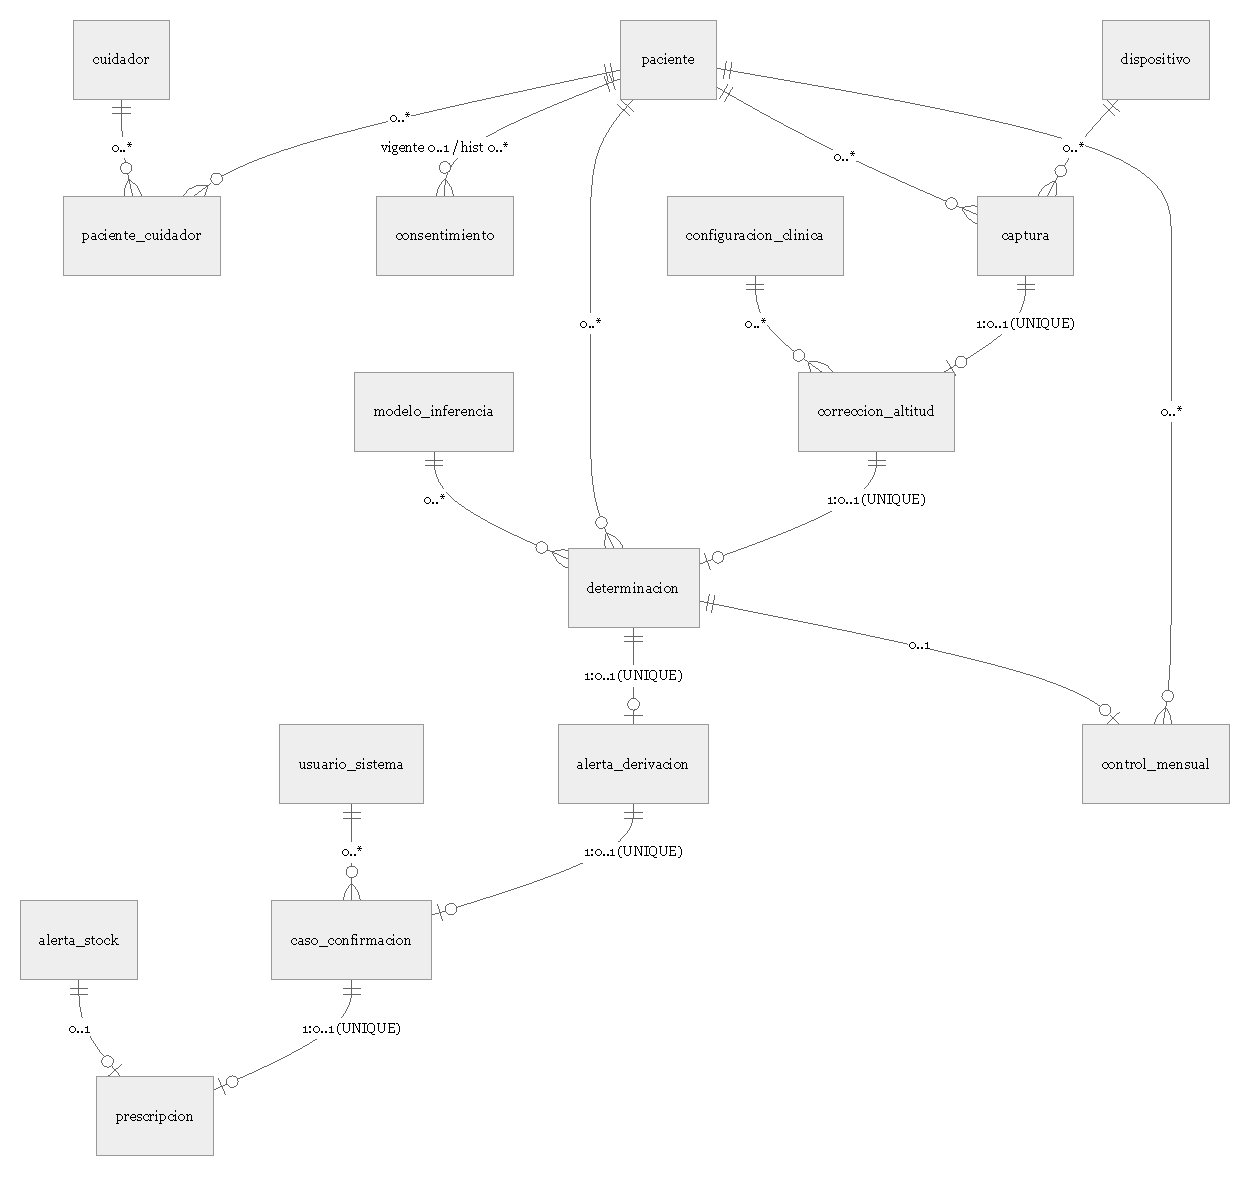
\includegraphics[width=0.98\linewidth,keepaspectratio]{assets/06-plataforma-datos/diagrama-02-er-nucleo-clinico.pdf}}
\end{figure}

\textbf{Diagrama 3 --- Resolución de la referencia polimórfica FHIR y trazabilidad de auditoría.}

\begin{figure}[H]
\centering
\pandocbounded{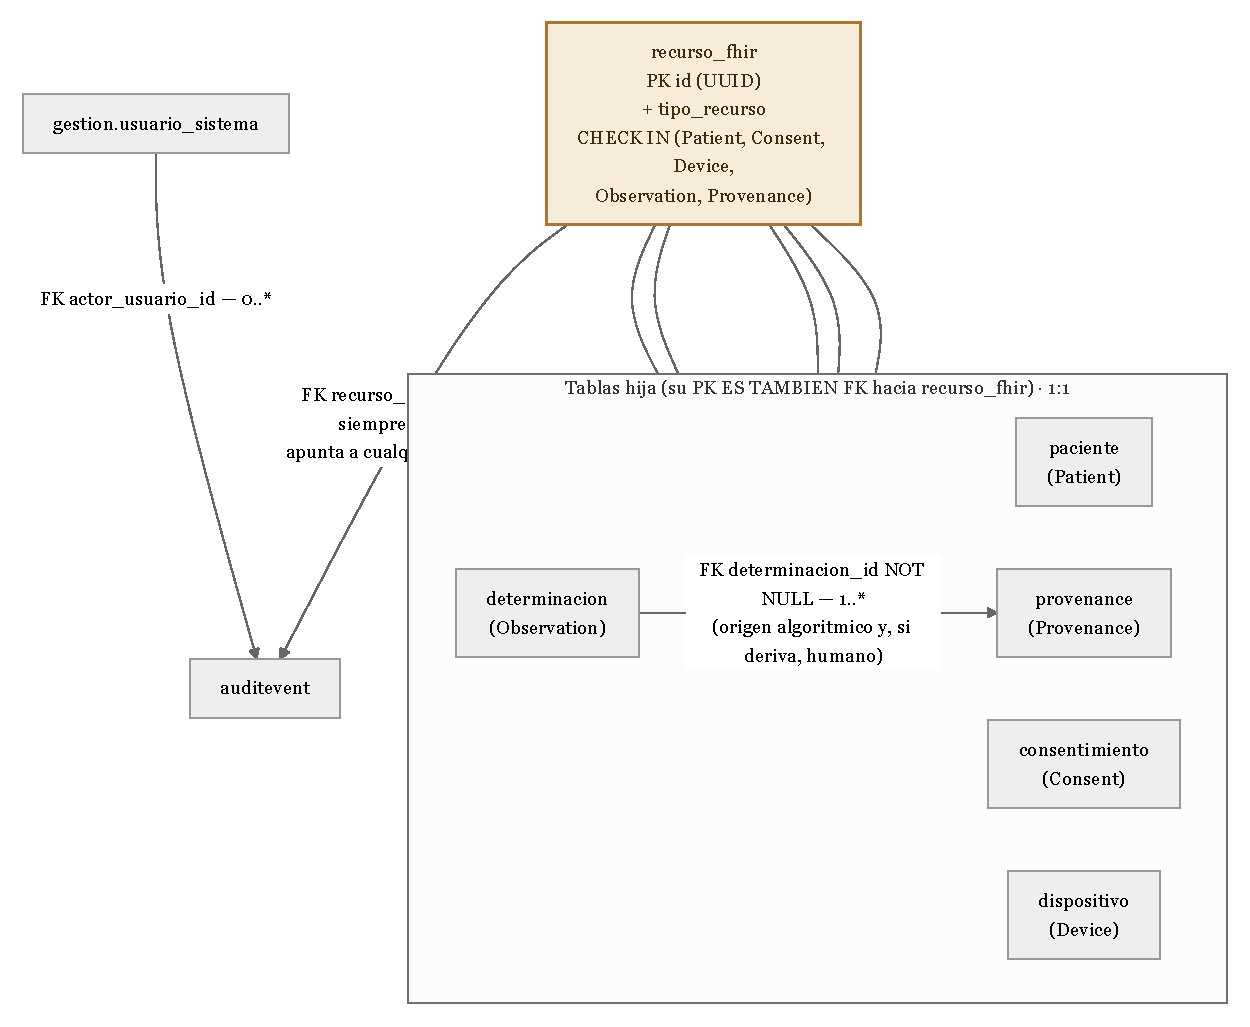
\includegraphics[width=0.9\linewidth,keepaspectratio]{assets/06-plataforma-datos/diagrama-03-fhir-polimorfica.pdf}}
\end{figure}

\textbf{Diagrama 4 --- Modelo E-R del dominio geoespacial (esquema \texttt{geo}, PostGIS).}

\begin{figure}[H]
\centering
\pandocbounded{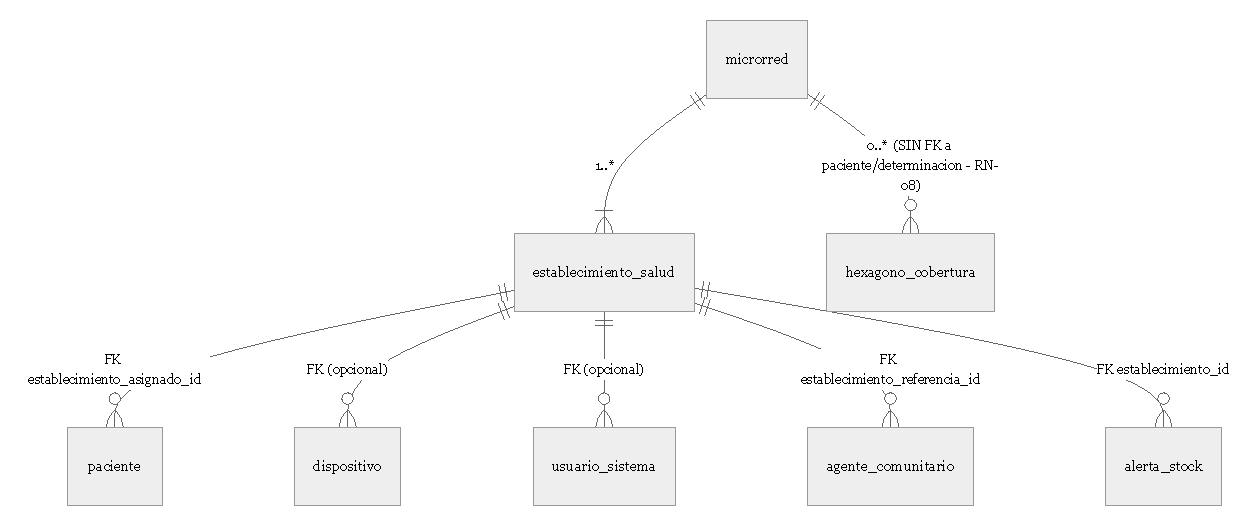
\includegraphics[width=0.85\linewidth,keepaspectratio]{assets/06-plataforma-datos/diagrama-04-er-geoespacial.pdf}}
\end{figure}

\textbf{Diagrama 5 --- Modelo E-R del dominio de configuración clínica y de gestión (esquemas \texttt{config} y \texttt{gestion}).}

\begin{figure}[H]
\centering
\pandocbounded{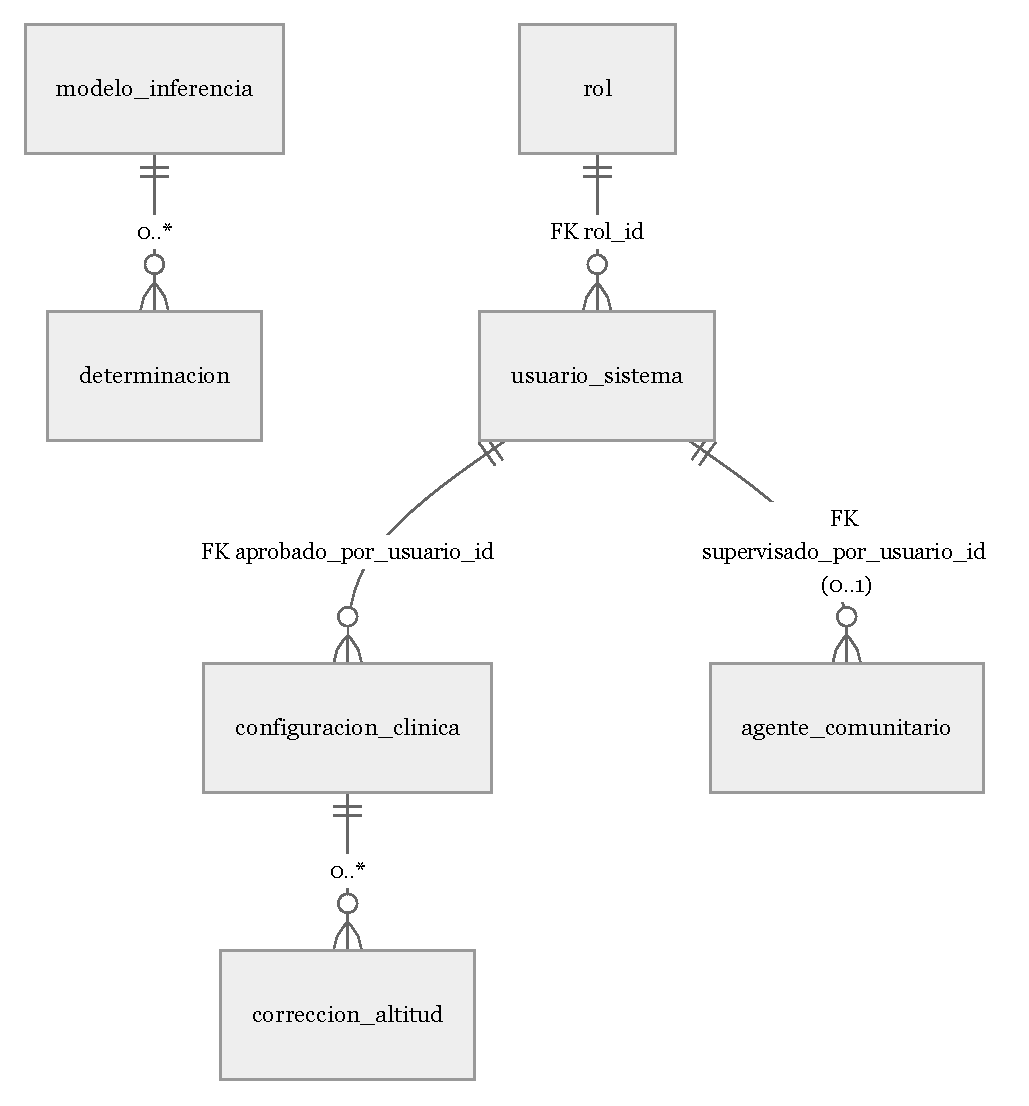
\includegraphics[width=0.8\linewidth,keepaspectratio]{assets/06-plataforma-datos/diagrama-05-er-config-gestion.pdf}}
\end{figure}

\subsection{1.4 Reconciliación con el Diagrama de Clases del Entregable N.° 5}\label{reconciliaciuxf3n-con-el-diagrama-de-clases-del-entregable-n.-5}

Esta sección es, deliberadamente, la más importante desde el punto de vista de la coherencia entre entregables: demuestra, clase por clase, que el modelo relacional de este documento \textbf{no diverge arbitrariamente} del diagrama de clases ya validado, sino que lo traduce con reglas explícitas y documentadas.

{\small
\begin{longtable}[]{@{}
  >{\raggedright\arraybackslash}p{(\linewidth - 4\tabcolsep) * \real{0.3333}}
  >{\raggedright\arraybackslash}p{(\linewidth - 4\tabcolsep) * \real{0.3333}}
  >{\raggedright\arraybackslash}p{(\linewidth - 4\tabcolsep) * \real{0.3333}}@{}}
\toprule\noalign{}
\begin{minipage}[b]{\linewidth}\raggedright
Clase del Diagrama 6 (Entregable N.° 5)
\end{minipage} & \begin{minipage}[b]{\linewidth}\raggedright
Tabla(s) de este modelo
\end{minipage} & \begin{minipage}[b]{\linewidth}\raggedright
Tipo de traducción
\end{minipage} \\
\midrule\noalign{}
\endhead
\bottomrule\noalign{}
\endlastfoot
Paciente & \texttt{clinico.paciente} (+ \texttt{clinico.recurso\_fhir}) & Directa, con adición de \texttt{nombres}/\texttt{apellidos} (ver nota A) \\
Cuidador & \texttt{clinico.cuidador} & Directa, con reubicación de \texttt{parentesco} (ver nota B) \\
Consentimiento (Consent) & \texttt{clinico.consentimiento} (+ \texttt{clinico.recurso\_fhir}) & Directa \\
Dispositivo (Device) & \texttt{clinico.dispositivo} (+ \texttt{clinico.recurso\_fhir}) & Directa \\
Captura & \texttt{clinico.captura} & Directa \\
CorreccionAltitud & \texttt{clinico.correccion\_altitud} & Directa \\
Determinacion (Observation) & \texttt{clinico.determinacion} (+ \texttt{clinico.recurso\_fhir}) & Directa \\
AlertaDerivacion & \texttt{clinico.alerta\_derivacion} & Directa \\
CasoConfirmacion & \texttt{clinico.caso\_confirmacion} & Directa \\
Prescripcion & \texttt{clinico.prescripcion} & Directa \\
AuditEvent & \texttt{clinico.auditevent} & Directa, con FK real hacia \texttt{recurso\_fhir} (ver nota C) \\
Provenance & \texttt{clinico.provenance} (+ \texttt{clinico.recurso\_fhir}) & Directa, con cardinalidad reconciliada (ver nota D) \\
ModeloInferencia & \texttt{config.modelo\_inferencia} & Directa \\
ConfiguracionClinica & \texttt{config.configuracion\_clinica} & Directa \\
AlertaStock & \texttt{gestion.alerta\_stock} & Directa \\
ControlMensual & \texttt{clinico.control\_mensual} & Directa \\
ReporteEvolucion & \texttt{clinico.reporte\_evolucion} (VISTA, no tabla) & Materializa literalmente la nota original: ``vista derivada, no persistida'' (ver nota E) \\
HexagonoCobertura (H3Cell) & \texttt{geo.hexagono\_cobertura} & Directa, se preserva explícitamente la ausencia de FK a Paciente (RN-08) \\
UsuarioSistema & \texttt{gestion.usuario\_sistema} & Directa \\
Rol & \texttt{gestion.rol} & Directa \\
\emph{(sin clase equivalente)} & \texttt{clinico.paciente\_cuidador} & \textbf{Tabla nueva}: resuelve la relación M:N Paciente-Cuidador, no representable como tabla propia en un diagrama de clases UML (allí es solo una asociación) \\
\emph{(sin clase equivalente)} & \texttt{clinico.recurso\_fhir} & \textbf{Tabla nueva} (técnica): resuelve la referencia polimórfica de AuditEvent con integridad real (ver nota C) \\
\emph{(sin clase equivalente)} & \texttt{geo.microrred}, \texttt{geo.establecimiento\_salud} & \textbf{Tablas nuevas}: la organización territorial estaba implícita (``establecimientoAsignado'' como atributo de tipo texto en Paciente) pero nunca modelada como entidad propia; CE022 exige explícitamente su normalización \\
\emph{(sin clase equivalente)} & \texttt{gestion.agente\_comunitario} & \textbf{Tabla nueva}: exigida por el alcance explícito de CE022 (``agentes comunitarios''); no existía como clase de software porque el Entregable N.° 5 solo modeló actores que operan directamente el sistema \\
\end{longtable}
}

\textbf{Nota A (Paciente --- nombres/apellidos).} El Diagrama 6 no listaba un atributo de nombre en \texttt{Paciente}. Este modelo lo añade porque es un requisito operativo real e ineludible de RF-04 (búsqueda del niño/a en la agenda del día, pantalla P04): sin un campo de nombre, la pantalla P03 (``Agenda del día'') no podría mostrar la lista ``Niño A --- CRED 6 meses'' que el propio prototipo del Entregable N.° 5 diseñó. Se documenta como una extensión necesaria, no como una corrección de un error del entregable anterior.

\textbf{Nota B (Cuidador --- reubicación de \texttt{parentesco}).} El Diagrama 6 listaba \texttt{parentesco} como atributo directo de \texttt{Cuidador}. Este modelo lo reubica como atributo de la tabla de unión \texttt{paciente\_cuidador}, porque el parentesco es una propiedad de la \textbf{relación} entre un cuidador y un paciente específico, no del cuidador en sí: una misma persona puede ser madre de un niño/a y tía de otro registrado en el mismo sistema. Este es un refinamiento propio de la normalización relacional (evita que el mismo cuidador con dos parentescos distintos requiera dos filas duplicadas de \texttt{Cuidador}), no posible de expresar con la misma precisión en un diagrama de clases simple.

\textbf{Nota C (AuditEvent --- integridad referencial real de la referencia polimórfica).} La sección 4.5 del Entregable N.° 5 estableció que \texttt{AuditEvent} ``puede referenciar a cualquiera de los otros cinco recursos, sin excepción'' (RN-11). Una traducción ingenua de esta regla a SQL usaría una columna \texttt{recurso\_id\ UUID} sin llave foránea (validada solo en la capa de aplicación), lo que \textbf{no} cumpliría el criterio de ``integridad referencial completa'' de la rúbrica de este entregable. Este modelo introduce en su lugar \texttt{clinico.recurso\_fhir}, una tabla técnica cuya clave primaria comparten \texttt{paciente}, \texttt{consentimiento}, \texttt{dispositivo}, \texttt{determinacion} y \texttt{provenance} (patrón de diseño conocido como \emph{Class Table Inheritance} o ``superclase de identificadores compartidos''): \texttt{auditevent.recurso\_id} es una FK real hacia \texttt{recurso\_fhir.id}, por lo que el motor de base de datos garantiza, sin posibilidad de excepción, que todo \texttt{AuditEvent} apunta a un recurso que efectivamente existe --- sin necesitar cinco columnas de FK nulificables (una trampa común de modelado que viola la Tercera Forma Normal al introducir columnas casi siempre nulas).

\textbf{Nota D (Provenance --- reconciliación de cardinalidad).} El Diagrama 6 dibuja, por una decisión de layout, una única relación de \texttt{CasoConfirmacion} hacia \texttt{Provenance} con cardinalidad \texttt{1:1}. Sin embargo, el texto de la sección 4.5 del mismo Entregable N.° 5 es más preciso y prevalece sobre el dibujo: \emph{``Provenance \textbar{} CorreccionAltitud (agente = sistema/algoritmo), CasoConfirmacion (agente = Personal médico) {[}\ldots{]} Siempre apunta a un Observation''}. Esto implica que puede existir \textbf{más de un} registro de \texttt{Provenance} por \texttt{Determinacion} (uno de origen algorítmico, generado siempre; y, si el caso se deriva y se confirma, un segundo de origen humano). Este modelo implementa fielmente el texto (cardinalidad \texttt{determinacion\ 1\ :\ provenance\ 1..*}, con \texttt{determinacion\_id\ NOT\ NULL}), documentando explícitamente esta reconciliación para que no se lea como una divergencia no intencional.

\textbf{Nota E (ReporteEvolucion --- de clase a vista).} El Diagrama 6 ya anotó esta clase como ``vista derivada, no persistida como recurso FHIR propio''. Este modelo cumple esa intención literalmente: \texttt{clinico.reporte\_evolucion} se implementa como una sentencia \texttt{CREATE\ VIEW} (Sección 2.2), no como una tabla con datos propios, evitando la duplicación de \texttt{hb\_observada}/\texttt{hb\_corregida}/\texttt{severidad} que ya existen en \texttt{correccion\_altitud} y \texttt{determinacion}.

\textbf{Nota de coherencia con ADR-06 (Location / \texttt{establecimiento\_salud}).} El ADR-06 del Entregable N.° 5 fijó el alcance de recursos FHIR \textbf{clínicos} de Fase 0 en exactamente seis (Patient, Consent, Device, Observation, Provenance, AuditEvent) y difirió explícitamente un séptimo (MedicationRequest) a Fase 1. La tabla \texttt{geo.establecimiento\_salud} introducida en este entregable \textbf{no contradice ese alcance}: no es un recurso FHIR clínico y no se cuenta dentro de los ``seis'' ya comprometidos. Es, en cambio, el equivalente funcional de un recurso FHIR \emph{Location} --- una entidad de apoyo administrativo-geográfico transversal en el estándar HL7 FHIR, no considerada parte del núcleo clínico de ningún proyecto---, que \textbf{podría} serializarse como \texttt{Location} si en el futuro se requiere para interoperabilidad con el HIS-MINSA (por ejemplo, referenciada desde \texttt{Patient.managingOrganization}), pero que en esta Parte 1 existe únicamente como tabla de apoyo del modelo relacional. Esta distinción se dedica una nota explícita porque el proyecto exige, como práctica consistente, verificar que ningún entregable nuevo contradiga los diez ADR ya fijados.

\subsection{1.5 Modelo lógico relacional}\label{modelo-luxf3gico-relacional}

La siguiente tabla resume, esquema por esquema, la estructura lógica de cada tabla: su llave primaria, sus llaves foráneas salientes y las restricciones distintivas que la caracterizan (el detalle exhaustivo columna por columna se desarrolla en el diccionario de datos, sección 1.7). Esta vista intermedia ---entre el diagrama conceptual (1.3) y el diccionario completo (1.7)--- es la que permite verificar de un vistazo que ninguna tabla queda sin llave primaria y que toda relación declarada en los diagramas E-R tiene su llave foránea correspondiente.

\textbf{Esquema \texttt{gestion}}

{\small
\begin{longtable}[]{@{}
  >{\raggedright\arraybackslash}p{(\linewidth - 6\tabcolsep) * \real{0.2500}}
  >{\raggedright\arraybackslash}p{(\linewidth - 6\tabcolsep) * \real{0.2500}}
  >{\raggedright\arraybackslash}p{(\linewidth - 6\tabcolsep) * \real{0.2500}}
  >{\raggedright\arraybackslash}p{(\linewidth - 6\tabcolsep) * \real{0.2500}}@{}}
\toprule\noalign{}
\begin{minipage}[b]{\linewidth}\raggedright
Tabla
\end{minipage} & \begin{minipage}[b]{\linewidth}\raggedright
PK
\end{minipage} & \begin{minipage}[b]{\linewidth}\raggedright
FK salientes
\end{minipage} & \begin{minipage}[b]{\linewidth}\raggedright
Restricciones distintivas
\end{minipage} \\
\midrule\noalign{}
\endhead
\bottomrule\noalign{}
\endlastfoot
\texttt{rol} & \texttt{id} (identity) & --- & \texttt{UNIQUE(nombre\_rol)}; \texttt{CHECK} de 7 valores admitidos \\
\texttt{usuario\_sistema} & \texttt{id} (UUID) & \texttt{rol\_id\ -\textgreater{}\ rol}; \texttt{establecimiento\_asignado\_id\ -\textgreater{}\ geo.establecimiento\_salud} & \texttt{UNIQUE(correo)}; \texttt{UNIQUE(keycloak\_subject\_id)} \\
\texttt{agente\_comunitario} & \texttt{id} (UUID) & \texttt{establecimiento\_referencia\_id\ -\textgreater{}\ geo.establecimiento\_salud}; \texttt{supervisado\_por\_usuario\_id\ -\textgreater{}\ usuario\_sistema} & --- \\
\texttt{alerta\_stock} & \texttt{id} (UUID) & \texttt{establecimiento\_id\ -\textgreater{}\ geo.establecimiento\_salud} & \texttt{CHECK} de estado y de valores no negativos \\
\end{longtable}
}

\textbf{Esquema \texttt{geo}}

{\small
\begin{longtable}[]{@{}
  >{\raggedright\arraybackslash}p{(\linewidth - 6\tabcolsep) * \real{0.2500}}
  >{\raggedright\arraybackslash}p{(\linewidth - 6\tabcolsep) * \real{0.2500}}
  >{\raggedright\arraybackslash}p{(\linewidth - 6\tabcolsep) * \real{0.2500}}
  >{\raggedright\arraybackslash}p{(\linewidth - 6\tabcolsep) * \real{0.2500}}@{}}
\toprule\noalign{}
\begin{minipage}[b]{\linewidth}\raggedright
Tabla
\end{minipage} & \begin{minipage}[b]{\linewidth}\raggedright
PK
\end{minipage} & \begin{minipage}[b]{\linewidth}\raggedright
FK salientes
\end{minipage} & \begin{minipage}[b]{\linewidth}\raggedright
Restricciones distintivas
\end{minipage} \\
\midrule\noalign{}
\endhead
\bottomrule\noalign{}
\endlastfoot
\texttt{microrred} & \texttt{id} (UUID) & --- & \texttt{CHECK(ubigeo\_departamento\ =\ \textquotesingle{}21\textquotesingle{})} \\
\texttt{establecimiento\_salud} & \texttt{id} (UUID) & \texttt{microrred\_id\ -\textgreater{}\ microrred} & \texttt{CHECK} de categoría (I-1..II-2); índice \texttt{GIST} sobre \texttt{ubicacion} \\
\texttt{hexagono\_cobertura} & \texttt{id} (UUID) & \texttt{microrred\_id\ -\textgreater{}\ microrred} & \texttt{UNIQUE(h3\_index,\ periodo\_inicio,\ periodo\_fin)}; \textbf{sin FK a paciente/determinacion} (RN-08) \\
\end{longtable}
}

\textbf{Esquema \texttt{config}}

{\small
\begin{longtable}[]{@{}
  >{\raggedright\arraybackslash}p{(\linewidth - 6\tabcolsep) * \real{0.2500}}
  >{\raggedright\arraybackslash}p{(\linewidth - 6\tabcolsep) * \real{0.2500}}
  >{\raggedright\arraybackslash}p{(\linewidth - 6\tabcolsep) * \real{0.2500}}
  >{\raggedright\arraybackslash}p{(\linewidth - 6\tabcolsep) * \real{0.2500}}@{}}
\toprule\noalign{}
\begin{minipage}[b]{\linewidth}\raggedright
Tabla
\end{minipage} & \begin{minipage}[b]{\linewidth}\raggedright
PK
\end{minipage} & \begin{minipage}[b]{\linewidth}\raggedright
FK salientes
\end{minipage} & \begin{minipage}[b]{\linewidth}\raggedright
Restricciones distintivas
\end{minipage} \\
\midrule\noalign{}
\endhead
\bottomrule\noalign{}
\endlastfoot
\texttt{modelo\_inferencia} & \texttt{id} (UUID) & --- & \texttt{UNIQUE(version)} \\
\texttt{configuracion\_clinica} & \texttt{id} (UUID) & \texttt{aprobado\_por\_usuario\_id\ -\textgreater{}\ gestion.usuario\_sistema} & \texttt{UNIQUE(tipo\_parametro,\ version)}; \textbf{índice único parcial} \texttt{uq\_config\_vigente} (una sola versión vigente por tipo --- materializa RN-02/CA-10) \\
\end{longtable}
}

\textbf{Esquema \texttt{clinico}}

{\small
\begin{longtable}[]{@{}
  >{\raggedright\arraybackslash}p{(\linewidth - 6\tabcolsep) * \real{0.2500}}
  >{\raggedright\arraybackslash}p{(\linewidth - 6\tabcolsep) * \real{0.2500}}
  >{\raggedright\arraybackslash}p{(\linewidth - 6\tabcolsep) * \real{0.2500}}
  >{\raggedright\arraybackslash}p{(\linewidth - 6\tabcolsep) * \real{0.2500}}@{}}
\toprule\noalign{}
\begin{minipage}[b]{\linewidth}\raggedright
Tabla
\end{minipage} & \begin{minipage}[b]{\linewidth}\raggedright
PK
\end{minipage} & \begin{minipage}[b]{\linewidth}\raggedright
FK salientes
\end{minipage} & \begin{minipage}[b]{\linewidth}\raggedright
Restricciones distintivas
\end{minipage} \\
\midrule\noalign{}
\endhead
\bottomrule\noalign{}
\endlastfoot
\texttt{recurso\_fhir} & \texttt{id} (UUID) & --- & \texttt{CHECK} de 5 tipos admitidos (superclase técnica, ver nota C, 1.4) \\
\texttt{paciente} & \texttt{id} (UUID, = FK a \texttt{recurso\_fhir}) & \texttt{id\ -\textgreater{}\ recurso\_fhir}; \texttt{establecimiento\_asignado\_id\ -\textgreater{}\ geo.establecimiento\_salud} & \texttt{UNIQUE(codigo\_padron\_nominal)}; \texttt{CHECK} de edad (\textless{} 6 años) \\
\texttt{cuidador} & \texttt{id} (UUID) & --- & \texttt{CHECK} de idioma (RNF-15) \\
\texttt{paciente\_cuidador} & \texttt{(paciente\_id,\ cuidador\_id)} compuesta & \texttt{paciente\_id\ -\textgreater{}\ paciente}; \texttt{cuidador\_id\ -\textgreater{}\ cuidador} & \texttt{ON\ DELETE\ CASCADE} (tabla de unión pura) \\
\texttt{consentimiento} & \texttt{id} (UUID, = FK a \texttt{recurso\_fhir}) & \texttt{paciente\_id\ -\textgreater{}\ paciente}; \texttt{cuidador\_id\ -\textgreater{}\ cuidador} & \textbf{índice único parcial} \texttt{uq\_consentimiento\_vigente\_por\_paciente} (materializa RN-04) \\
\texttt{dispositivo} & \texttt{id} (UUID, = FK a \texttt{recurso\_fhir}) & \texttt{establecimiento\_asignado\_id\ -\textgreater{}\ geo.establecimiento\_salud} & \texttt{UNIQUE(numero\_serie)} \\
\texttt{captura} & \texttt{id} (UUID) & \texttt{paciente\_id\ -\textgreater{}\ paciente}; \texttt{dispositivo\_id\ -\textgreater{}\ dispositivo}; \texttt{capturado\_por\_usuario\_id\ -\textgreater{}\ gestion.usuario\_sistema} & \texttt{CHECK(array\_length(espectro\_as7341,1)=11)}; índice \texttt{GIST} sobre \texttt{coordenada\_gps} \\
\texttt{correccion\_altitud} & \texttt{id} (UUID) & \texttt{captura\_id\ -\textgreater{}\ captura} (\textbf{UNIQUE}, fuerza 1:1); \texttt{configuracion\_clinica\_id\ -\textgreater{}\ config.configuracion\_clinica} & \texttt{CHECK} de rangos de altitud y de Hb \\
\texttt{determinacion} & \texttt{id} (UUID, = FK a \texttt{recurso\_fhir}) & \texttt{paciente\_id\ -\textgreater{}\ paciente}; \texttt{correccion\_altitud\_id\ -\textgreater{}\ correccion\_altitud} (\textbf{UNIQUE}); \texttt{dispositivo\_id\ -\textgreater{}\ dispositivo}; \texttt{modelo\_inferencia\_id\ -\textgreater{}\ config.modelo\_inferencia} & \texttt{CHECK} de severidad (4 valores) y de estado (9 valores, igual al Diagrama 11) \\
\texttt{alerta\_derivacion} & \texttt{id} (UUID) & \texttt{determinacion\_id\ -\textgreater{}\ determinacion} (\textbf{UNIQUE}) & \texttt{CHECK} de severidad y estado \\
\texttt{caso\_confirmacion} & \texttt{id} (UUID) & \texttt{alerta\_derivacion\_id\ -\textgreater{}\ alerta\_derivacion} (\textbf{UNIQUE}); \texttt{profesional\_usuario\_id\ -\textgreater{}\ gestion.usuario\_sistema} & \texttt{CHECK} de resultado y modalidad \\
\texttt{prescripcion} & \texttt{id} (UUID) & \texttt{caso\_confirmacion\_id\ -\textgreater{}\ caso\_confirmacion} (\textbf{UNIQUE}); \texttt{alerta\_stock\_id\ -\textgreater{}\ gestion.alerta\_stock} & --- \\
\texttt{provenance} & \texttt{id} (UUID, = FK a \texttt{recurso\_fhir}) & \texttt{determinacion\_id\ -\textgreater{}\ determinacion} (\textbf{NOT NULL}, no UNIQUE); \texttt{agente\_usuario\_id\ -\textgreater{}\ gestion.usuario\_sistema} & \texttt{CHECK} de origen y tipo de agente \\
\texttt{auditevent} & \texttt{id} (UUID) & \texttt{recurso\_id\ -\textgreater{}\ recurso\_fhir}; \texttt{actor\_usuario\_id\ -\textgreater{}\ gestion.usuario\_sistema} & \texttt{CHECK} de acción (CRUD) y resultado \\
\texttt{control\_mensual} & \texttt{id} (UUID) & \texttt{paciente\_id\ -\textgreater{}\ paciente}; \texttt{determinacion\_id\ -\textgreater{}\ determinacion} (UNIQUE, nulable) & \texttt{UNIQUE(paciente\_id,\ numero\_control)} \\
\end{longtable}
}

\textbf{Vista derivada:} \texttt{clinico.reporte\_evolucion} (sin PK propia; \texttt{SELECT} sobre \texttt{paciente} + \texttt{determinacion} + \texttt{correccion\_altitud}).

\subsection{1.6 Modelo normalizado: prueba de Primera, Segunda y Tercera Forma Normal}\label{modelo-normalizado-prueba-de-primera-segunda-y-tercera-forma-normal}

Se demuestra el cumplimiento de 1FN, 2FN y 3FN sobre cuatro tablas representativas ---elegidas por cubrir los casos más exigentes del esquema (llave compuesta, llave que no es UUID simple, columna de tipo arreglo y columna JSONB)--- y se declara que la misma disciplina de diseño se aplicó, sin excepción, al resto de las 24 tablas.

\textbf{\texttt{clinico.paciente\_cuidador} (caso de llave compuesta).}
- \emph{1FN:} todos los atributos (\texttt{paciente\_id}, \texttt{cuidador\_id}, \texttt{parentesco}, \texttt{es\_contacto\_principal}) son atómicos y de un solo valor; no hay grupos repetitivos. Cumple.
- \emph{2FN:} la llave primaria es compuesta (\texttt{paciente\_id}, \texttt{cuidador\_id}). \texttt{parentesco} y \texttt{es\_contacto\_principal} dependen de \textbf{ambas} columnas de la llave a la vez (el parentesco es una propiedad del par específico paciente-cuidador, no de uno solo) --- no existe dependencia parcial de solo una parte de la llave. Cumple.
- \emph{3FN:} no existen dependencias transitivas (ningún atributo no clave determina a otro atributo no clave). Cumple.

\textbf{\texttt{clinico.determinacion} (caso de núcleo clínico con múltiples FK).}
- \emph{1FN:} atributos atómicos (\texttt{valor\_hb\_final}, \texttt{severidad}, \texttt{estado}, \texttt{fecha\_creacion}); ningún atributo agrupa múltiples valores. Cumple.
- \emph{2FN:} la llave primaria es simple (\texttt{id}), por lo que no aplica el caso de dependencia parcial (solo es relevante con llaves compuestas); se cumple trivialmente.
- \emph{3FN:} se verificó explícitamente que ningún atributo no clave depende de otro atributo no clave. Un caso límite discutido y descartado: \texttt{severidad} podría \emph{parecer} derivable de \texttt{valor\_hb\_final} mediante los cortes de \texttt{config.configuracion\_clinica}, lo que sugeriría una dependencia transitiva. Se decidió \textbf{mantener \texttt{severidad} como columna propia} (no derivarla en tiempo de consulta) porque los cortes de severidad son ellos mismos versionados en el tiempo (\texttt{config.configuracion\_clinica}); si se recalculara \texttt{severidad} en cada consulta contra la versión \emph{vigente} de los cortes, una determinación histórica cambiaría retroactivamente de clasificación cada vez que se actualice la tabla de cortes, lo cual violaría directamente la trazabilidad exigida por RN-02 y CA-10 (``mantener trazabilidad de qué versión se aplicó a cada determinación histórica''). Esta es una \textbf{desnormalización deliberada y documentada}, no un descuido: se prioriza la inmutabilidad histórica exigida por una regla de negocio explícita sobre la pureza normalizadora estricta.

\textbf{\texttt{clinico.captura} (caso de columna de tipo arreglo).}
- \emph{1FN (discusión explícita):} la columna \texttt{espectro\_as7341\ NUMERIC(10,4){[}{]}} es, en sentido estricto de la teoría relacional clásica, un caso límite de 1FN, que exige valores atómicos y prohíbe ``grupos repetitivos''. La alternativa estrictamente normalizada sería una tabla hija \texttt{captura\_canal\_espectral(captura\_id,\ indice\_canal,\ valor)} con 11 filas por captura. Se evaluaron ambas opciones y se optó deliberadamente por el arreglo de tamaño fijo, por tres razones documentadas: (i) los 11 canales del sensor AS7341 siempre se leen y se escriben como una unidad atómica de dominio --- nunca se consulta o actualiza un canal de forma aislada de los otros diez ---, por lo que conceptualmente se comportan como un único valor compuesto (análogo a como \texttt{coordenada\_gps\ geography(Point)} también es, en rigor, un par de coordenadas, pero se trata como un tipo atómico de dominio geoespacial); (ii) PostgreSQL ofrece soporte nativo, indexable y con validación de longitud (\texttt{array\_length(...)\ =\ 11}) para este patrón, sin las siete llaves foráneas adicionales y el \texttt{JOIN} obligatorio que exigiría la alternativa normalizada; y (iii) el propio Entregable N.° 5 (RF-02) define el espectro como una unidad de captura sincronizada de ``11 canales'', reforzando que el dominio del problema ya lo trata como un valor compuesto único. Se documenta esta decisión explícitamente como una \textbf{excepción justificada y acotada} a la 1FN estricta, no como un patrón a repetir libremente en el resto del esquema (ninguna otra tabla usa arreglos).
- \emph{2FN y 3FN:} con llave primaria simple (\texttt{id}) y sin dependencias transitivas entre \texttt{paciente\_id}, \texttt{dispositivo\_id}, \texttt{marca\_tiempo}, \texttt{calidad\_senal}, etc., ambas formas se cumplen sin excepción.

\textbf{\texttt{config.configuracion\_clinica} (caso de columna JSONB).}
- \emph{1FN (discusión explícita):} \texttt{valor\_versionado\ JSONB} almacena una estructura semi-estructurada (p.~ej. los tramos de la fórmula de corrección por altitud), que podría interpretarse como una violación de la atomicidad de 1FN. Se justifica de forma análoga al caso anterior: el \textbf{contenido interno} de esa estructura todavía no está definido con exactitud (depende del texto íntegro, aún pendiente, de la NTS 213-MINSA/DGIESP-2024 --- RN-02), por lo que fijar columnas rígidas para ``tramo 1'', ``tramo 2'', etc. sería una normalización prematura sobre datos cuya forma exacta se desconoce. JSONB se usa aquí exactamente para el propósito que la regla de negocio RN-02 exige: permitir que el parámetro sea ``parametrizable, versionado y auditable'' sin fijar su forma en el esquema. Esta misma justificación aplica a \texttt{modelo\_inferencia.metricas}, \texttt{gestion.rol.permisos}, \texttt{clinico.consentimiento.alcance}, \texttt{clinico.prescripcion.anotacion\_estructurada} y \texttt{clinico.auditevent.detalle}.
- \emph{2FN y 3FN:} se cumplen sin excepción (llave simple, sin dependencias transitivas entre \texttt{tipo\_parametro}, \texttt{version}, \texttt{fecha\_vigencia\_desde/hasta} y \texttt{aprobado\_por\_usuario\_id}).

\textbf{Declaración general.} Las 20 tablas restantes del esquema no presentan ninguno de los dos casos límite discutidos (llave compuesta con dependencia parcial potencial, o columnas de tipo no escalar) y cumplen 1FN, 2FN y 3FN de forma directa: cada una tiene una llave primaria simple de tipo \texttt{UUID} (o \texttt{SMALLINT\ IDENTITY} en el caso de \texttt{rol}), todos sus atributos no clave dependen funcionalmente de esa llave completa, y no se identificó ninguna dependencia transitiva entre atributos no clave.

\subsection{1.7 Diccionario de datos completo}\label{diccionario-de-datos-completo}

Se documentan las 24 tablas y la vista derivada, agrupadas por esquema en el mismo orden de creación del script DDL (Sección 2.2, Anexo A). Columnas: \textbf{Nulo} indica si la columna admite \texttt{NULL} (No = \texttt{NOT\ NULL}); \textbf{Clave} indica \texttt{PK} (llave primaria), \texttt{FK-\textgreater{}tabla} (llave foránea y su tabla referenciada) o \texttt{UQ} (restricción \texttt{UNIQUE} no relacionada a llave).

\subsubsection{\texorpdfstring{Esquema \texttt{gestion}}{Esquema gestion}}\label{esquema-gestion}

\textbf{\texttt{gestion.rol}} --- Catálogo RBAC (RF-37, RNF-06); la fuente de verdad de autenticación es Keycloak/OIDC (ADR-09).

{\small
\begin{longtable}[]{@{}
  >{\raggedright\arraybackslash}p{(\linewidth - 8\tabcolsep) * \real{0.2000}}
  >{\raggedright\arraybackslash}p{(\linewidth - 8\tabcolsep) * \real{0.2000}}
  >{\raggedright\arraybackslash}p{(\linewidth - 8\tabcolsep) * \real{0.2000}}
  >{\raggedright\arraybackslash}p{(\linewidth - 8\tabcolsep) * \real{0.2000}}
  >{\raggedright\arraybackslash}p{(\linewidth - 8\tabcolsep) * \real{0.2000}}@{}}
\toprule\noalign{}
\begin{minipage}[b]{\linewidth}\raggedright
Columna
\end{minipage} & \begin{minipage}[b]{\linewidth}\raggedright
Tipo
\end{minipage} & \begin{minipage}[b]{\linewidth}\raggedright
Nulo
\end{minipage} & \begin{minipage}[b]{\linewidth}\raggedright
Clave
\end{minipage} & \begin{minipage}[b]{\linewidth}\raggedright
Descripción
\end{minipage} \\
\midrule\noalign{}
\endhead
\bottomrule\noalign{}
\endlastfoot
id & SMALLINT (identity) & No & PK & Identificador autogenerado \\
nombre\_rol & VARCHAR(30) & No & UQ & Uno de 7 valores: \texttt{personal\_cred}, \texttt{personal\_medico}, \texttt{farmacia}, \texttt{jefatura\_microred}, \texttt{analista\_diresa}, \texttt{administrador}, \texttt{auditor} \\
descripcion & VARCHAR(200) & No & --- & Descripción funcional del rol \\
permisos & JSONB & No & --- & Lista de permisos granulares (ver nota JSONB, sección 1.6) \\
\end{longtable}
}

\textbf{\texttt{gestion.usuario\_sistema}} --- Usuario interno (personal CRED, médico, farmacia, jefatura, analista, administrador, auditor).

{\small
\begin{longtable}[]{@{}
  >{\raggedright\arraybackslash}p{(\linewidth - 8\tabcolsep) * \real{0.2000}}
  >{\raggedright\arraybackslash}p{(\linewidth - 8\tabcolsep) * \real{0.2000}}
  >{\raggedright\arraybackslash}p{(\linewidth - 8\tabcolsep) * \real{0.2000}}
  >{\raggedright\arraybackslash}p{(\linewidth - 8\tabcolsep) * \real{0.2000}}
  >{\raggedright\arraybackslash}p{(\linewidth - 8\tabcolsep) * \real{0.2000}}@{}}
\toprule\noalign{}
\begin{minipage}[b]{\linewidth}\raggedright
Columna
\end{minipage} & \begin{minipage}[b]{\linewidth}\raggedright
Tipo
\end{minipage} & \begin{minipage}[b]{\linewidth}\raggedright
Nulo
\end{minipage} & \begin{minipage}[b]{\linewidth}\raggedright
Clave
\end{minipage} & \begin{minipage}[b]{\linewidth}\raggedright
Descripción
\end{minipage} \\
\midrule\noalign{}
\endhead
\bottomrule\noalign{}
\endlastfoot
id & UUID & No & PK & Identificador \\
nombre\_completo & VARCHAR(150) & No & --- & Nombre del usuario (dato ilustrativo en Fase 0) \\
correo & VARCHAR(150) & No & UQ & Correo institucional \\
rol\_id & SMALLINT & No & FK-\textgreater{}\texttt{gestion.rol} & Rol RBAC asignado \\
establecimiento\_asignado\_id & UUID & Sí & FK-\textgreater{}\texttt{geo.establecimiento\_salud} & Establecimiento base del usuario \\
keycloak\_subject\_id & VARCHAR(100) & Sí & UQ & Enlace al \texttt{sub} del token OIDC (ADR-09) \\
estado\_cuenta & VARCHAR(12) & No & --- & \texttt{activo} / \texttt{inactivo} / \texttt{suspendido} \\
creado\_en & TIMESTAMPTZ & No & --- & Auditoría técnica de creación del registro \\
\end{longtable}
}

\textbf{\texttt{gestion.agente\_comunitario}} --- Agente Comunitario de Salud (ACS); entidad nueva de este entregable (ver nota, sección 1.4).

{\small
\begin{longtable}[]{@{}
  >{\raggedright\arraybackslash}p{(\linewidth - 8\tabcolsep) * \real{0.2000}}
  >{\raggedright\arraybackslash}p{(\linewidth - 8\tabcolsep) * \real{0.2000}}
  >{\raggedright\arraybackslash}p{(\linewidth - 8\tabcolsep) * \real{0.2000}}
  >{\raggedright\arraybackslash}p{(\linewidth - 8\tabcolsep) * \real{0.2000}}
  >{\raggedright\arraybackslash}p{(\linewidth - 8\tabcolsep) * \real{0.2000}}@{}}
\toprule\noalign{}
\begin{minipage}[b]{\linewidth}\raggedright
Columna
\end{minipage} & \begin{minipage}[b]{\linewidth}\raggedright
Tipo
\end{minipage} & \begin{minipage}[b]{\linewidth}\raggedright
Nulo
\end{minipage} & \begin{minipage}[b]{\linewidth}\raggedright
Clave
\end{minipage} & \begin{minipage}[b]{\linewidth}\raggedright
Descripción
\end{minipage} \\
\midrule\noalign{}
\endhead
\bottomrule\noalign{}
\endlastfoot
id & UUID & No & PK & Identificador \\
nombre\_completo & VARCHAR(150) & No & --- & Nombre del agente comunitario \\
documento\_identidad\_hash & VARCHAR(128) & Sí & --- & Hash del documento de identidad, nunca en claro (Ley N.° 29733); mecanismo exacto {[}DATO PENDIENTE DE VALIDAR{]} \\
establecimiento\_referencia\_id & UUID & No & FK-\textgreater{}\texttt{geo.establecimiento\_salud} & Establecimiento al que reporta \\
supervisado\_por\_usuario\_id & UUID & Sí & FK-\textgreater{}\texttt{gestion.usuario\_sistema} & Personal CRED que lo supervisa \\
telefono\_contacto & VARCHAR(20) & Sí & --- & Contacto \\
zona\_cobertura\_descripcion & VARCHAR(200) & Sí & --- & Descripción textual de su zona de cobertura \\
fecha\_capacitacion & DATE & Sí & --- & Última capacitación registrada \\
estado\_activo & BOOLEAN & No & --- & Activo/inactivo \\
creado\_en & TIMESTAMPTZ & No & --- & Auditoría técnica \\
\end{longtable}
}

\textbf{\texttt{gestion.alerta\_stock}} --- Alerta de quiebre de stock de insumos de hierro (RF-25, RF-26).

{\small
\begin{longtable}[]{@{}
  >{\raggedright\arraybackslash}p{(\linewidth - 8\tabcolsep) * \real{0.2000}}
  >{\raggedright\arraybackslash}p{(\linewidth - 8\tabcolsep) * \real{0.2000}}
  >{\raggedright\arraybackslash}p{(\linewidth - 8\tabcolsep) * \real{0.2000}}
  >{\raggedright\arraybackslash}p{(\linewidth - 8\tabcolsep) * \real{0.2000}}
  >{\raggedright\arraybackslash}p{(\linewidth - 8\tabcolsep) * \real{0.2000}}@{}}
\toprule\noalign{}
\begin{minipage}[b]{\linewidth}\raggedright
Columna
\end{minipage} & \begin{minipage}[b]{\linewidth}\raggedright
Tipo
\end{minipage} & \begin{minipage}[b]{\linewidth}\raggedright
Nulo
\end{minipage} & \begin{minipage}[b]{\linewidth}\raggedright
Clave
\end{minipage} & \begin{minipage}[b]{\linewidth}\raggedright
Descripción
\end{minipage} \\
\midrule\noalign{}
\endhead
\bottomrule\noalign{}
\endlastfoot
id & UUID & No & PK & Identificador \\
establecimiento\_id & UUID & No & FK-\textgreater{}\texttt{geo.establecimiento\_salud} & Establecimiento afectado \\
insumo & VARCHAR(100) & No & --- & Insumo (por defecto ``Sulfato ferroso'') \\
stock\_proyectado & NUMERIC(10,2) & No & --- & Consumo proyectado \\
stock\_disponible & NUMERIC(10,2) & No & --- & Stock actual \\
estado & VARCHAR(20) & No & --- & \texttt{abierta} / \texttt{atendida} / \texttt{descartada} \\
fecha\_generacion & TIMESTAMPTZ & No & --- & Fecha de generación de la alerta \\
fecha\_resolucion & TIMESTAMPTZ & Sí & --- & Fecha de cierre, si aplica \\
\end{longtable}
}

\subsubsection{\texorpdfstring{Esquema \texttt{geo}}{Esquema geo}}\label{esquema-geo}

\textbf{\texttt{geo.microrred}} --- Unidad organizacional MINSA; caso ilustrativo ``Microred de Salud Altiplano-Puno''.

{\small
\begin{longtable}[]{@{}
  >{\raggedright\arraybackslash}p{(\linewidth - 8\tabcolsep) * \real{0.2000}}
  >{\raggedright\arraybackslash}p{(\linewidth - 8\tabcolsep) * \real{0.2000}}
  >{\raggedright\arraybackslash}p{(\linewidth - 8\tabcolsep) * \real{0.2000}}
  >{\raggedright\arraybackslash}p{(\linewidth - 8\tabcolsep) * \real{0.2000}}
  >{\raggedright\arraybackslash}p{(\linewidth - 8\tabcolsep) * \real{0.2000}}@{}}
\toprule\noalign{}
\begin{minipage}[b]{\linewidth}\raggedright
Columna
\end{minipage} & \begin{minipage}[b]{\linewidth}\raggedright
Tipo
\end{minipage} & \begin{minipage}[b]{\linewidth}\raggedright
Nulo
\end{minipage} & \begin{minipage}[b]{\linewidth}\raggedright
Clave
\end{minipage} & \begin{minipage}[b]{\linewidth}\raggedright
Descripción
\end{minipage} \\
\midrule\noalign{}
\endhead
\bottomrule\noalign{}
\endlastfoot
id & UUID & No & PK & Identificador \\
nombre & VARCHAR(150) & No & --- & Nombre de la microred \\
red\_salud & VARCHAR(150) & No & --- & Red de salud a la que pertenece (referencial) \\
diresa\_geresa & VARCHAR(150) & No & --- & DIRESA/GERESA responsable (referencial) \\
ubigeo\_departamento & CHAR(2) & No & --- & \texttt{21} = Puno (único valor válido) \\
ubigeo\_provincia & CHAR(4) & Sí & --- & {[}DATO PENDIENTE DE VALIDAR: exacto de la microred real{]} \\
creado\_en & TIMESTAMPTZ & No & --- & Auditoría técnica \\
\end{longtable}
}

\textbf{\texttt{geo.establecimiento\_salud}} --- Establecimiento de salud; equivalente funcional a FHIR \emph{Location} (ver nota ADR-06, sección 1.4).

{\small
\begin{longtable}[]{@{}
  >{\raggedright\arraybackslash}p{(\linewidth - 8\tabcolsep) * \real{0.2000}}
  >{\raggedright\arraybackslash}p{(\linewidth - 8\tabcolsep) * \real{0.2000}}
  >{\raggedright\arraybackslash}p{(\linewidth - 8\tabcolsep) * \real{0.2000}}
  >{\raggedright\arraybackslash}p{(\linewidth - 8\tabcolsep) * \real{0.2000}}
  >{\raggedright\arraybackslash}p{(\linewidth - 8\tabcolsep) * \real{0.2000}}@{}}
\toprule\noalign{}
\begin{minipage}[b]{\linewidth}\raggedright
Columna
\end{minipage} & \begin{minipage}[b]{\linewidth}\raggedright
Tipo
\end{minipage} & \begin{minipage}[b]{\linewidth}\raggedright
Nulo
\end{minipage} & \begin{minipage}[b]{\linewidth}\raggedright
Clave
\end{minipage} & \begin{minipage}[b]{\linewidth}\raggedright
Descripción
\end{minipage} \\
\midrule\noalign{}
\endhead
\bottomrule\noalign{}
\endlastfoot
id & UUID & No & PK & Identificador \\
microrred\_id & UUID & No & FK-\textgreater{}\texttt{geo.microrred} & Microred a la que pertenece \\
nombre & VARCHAR(150) & No & --- & Nombre del establecimiento \\
categoria & VARCHAR(10) & No & --- & I-1, I-2, I-3, I-4, II-1 o II-2 \\
codigo\_renaes & VARCHAR(20) & Sí & --- & {[}DATO PENDIENTE DE VALIDAR{]} \\
ubigeo & CHAR(6) & Sí & --- & {[}DATO PENDIENTE DE VALIDAR: distrital exacto{]} \\
ubicacion & geography(Point,4326) & No & --- & Coordenada PostGIS (punto de tamizaje fijo del establecimiento) \\
altitud\_referencia\_msnm & NUMERIC(6,1) & No & --- & Altitud oficial, derivada de MDE --- \textbf{nunca de GPS crudo} (RN-03) \\
fuente\_altitud & VARCHAR(20) & No & --- & \texttt{MDE} (default) o \texttt{GPS\_provisional} \\
es\_cabecera\_microrred & BOOLEAN & No & --- & Marca el establecimiento sede jefatural \\
creado\_en & TIMESTAMPTZ & No & --- & Auditoría técnica \\
\end{longtable}
}

\textbf{\texttt{geo.hexagono\_cobertura}} --- Capa agregada H3 (RF-33, RF-34); materializa RN-08 en el esquema.

{\small
\begin{longtable}[]{@{}
  >{\raggedright\arraybackslash}p{(\linewidth - 8\tabcolsep) * \real{0.2000}}
  >{\raggedright\arraybackslash}p{(\linewidth - 8\tabcolsep) * \real{0.2000}}
  >{\raggedright\arraybackslash}p{(\linewidth - 8\tabcolsep) * \real{0.2000}}
  >{\raggedright\arraybackslash}p{(\linewidth - 8\tabcolsep) * \real{0.2000}}
  >{\raggedright\arraybackslash}p{(\linewidth - 8\tabcolsep) * \real{0.2000}}@{}}
\toprule\noalign{}
\begin{minipage}[b]{\linewidth}\raggedright
Columna
\end{minipage} & \begin{minipage}[b]{\linewidth}\raggedright
Tipo
\end{minipage} & \begin{minipage}[b]{\linewidth}\raggedright
Nulo
\end{minipage} & \begin{minipage}[b]{\linewidth}\raggedright
Clave
\end{minipage} & \begin{minipage}[b]{\linewidth}\raggedright
Descripción
\end{minipage} \\
\midrule\noalign{}
\endhead
\bottomrule\noalign{}
\endlastfoot
id & UUID & No & PK & Identificador \\
h3\_index & VARCHAR(16) & No & --- & Índice H3 (Uber), formato hexadecimal \\
resolucion\_h3 & SMALLINT & No & --- & Resolución H3 (5 a 9); por defecto 7 \\
microrred\_id & UUID & No & FK-\textgreater{}\texttt{geo.microrred} & Microred de referencia \\
centroide & geography(Point,4326) & Sí & --- & Centroide del hexágono (para renderizado en el mapa) \\
periodo\_inicio & DATE & No & --- & Inicio del periodo agregado \\
periodo\_fin & DATE & No & --- & Fin del periodo agregado \\
tamizajes\_total & INTEGER & No & --- & Conteo agregado (nunca identificadores individuales) \\
derivaciones\_total & INTEGER & No & --- & Conteo agregado de derivaciones \\
prevalencia\_estimada & NUMERIC(5,2) & Sí & --- & Porcentaje estimado \\
ultima\_actualizacion & TIMESTAMPTZ & No & --- & Última corrida del proceso ETL que la actualizó \\
\end{longtable}
}

\subsubsection{\texorpdfstring{Esquema \texttt{config}}{Esquema config}}\label{esquema-config}

\textbf{\texttt{config.modelo\_inferencia}} --- Versión del modelo de inferencia embebido (RF-11, ADR-04).

{\small
\begin{longtable}[]{@{}
  >{\raggedright\arraybackslash}p{(\linewidth - 8\tabcolsep) * \real{0.2000}}
  >{\raggedright\arraybackslash}p{(\linewidth - 8\tabcolsep) * \real{0.2000}}
  >{\raggedright\arraybackslash}p{(\linewidth - 8\tabcolsep) * \real{0.2000}}
  >{\raggedright\arraybackslash}p{(\linewidth - 8\tabcolsep) * \real{0.2000}}
  >{\raggedright\arraybackslash}p{(\linewidth - 8\tabcolsep) * \real{0.2000}}@{}}
\toprule\noalign{}
\begin{minipage}[b]{\linewidth}\raggedright
Columna
\end{minipage} & \begin{minipage}[b]{\linewidth}\raggedright
Tipo
\end{minipage} & \begin{minipage}[b]{\linewidth}\raggedright
Nulo
\end{minipage} & \begin{minipage}[b]{\linewidth}\raggedright
Clave
\end{minipage} & \begin{minipage}[b]{\linewidth}\raggedright
Descripción
\end{minipage} \\
\midrule\noalign{}
\endhead
\bottomrule\noalign{}
\endlastfoot
id & UUID & No & PK & Identificador \\
version & VARCHAR(20) & No & UQ & Versión semántica del modelo \\
formato & VARCHAR(10) & No & --- & \texttt{ONNX} o \texttt{TFLite} \\
fecha\_entrenamiento & DATE & Sí & --- & Fecha de entrenamiento \\
metricas & JSONB & No & --- & Métricas de desempeño (p.~ej. MAE); valores exactos {[}DATO PENDIENTE DE VALIDAR{]} \\
activo & BOOLEAN & No & --- & Versión vigente distribuida a dispositivos \\
creado\_en & TIMESTAMPTZ & No & --- & Auditoría técnica \\
\end{longtable}
}

\textbf{\texttt{config.configuracion\_clinica}} --- Parámetros clínicos versionados (RN-02); tabla de corrección por altitud y umbrales de severidad.

{\small
\begin{longtable}[]{@{}
  >{\raggedright\arraybackslash}p{(\linewidth - 8\tabcolsep) * \real{0.2000}}
  >{\raggedright\arraybackslash}p{(\linewidth - 8\tabcolsep) * \real{0.2000}}
  >{\raggedright\arraybackslash}p{(\linewidth - 8\tabcolsep) * \real{0.2000}}
  >{\raggedright\arraybackslash}p{(\linewidth - 8\tabcolsep) * \real{0.2000}}
  >{\raggedright\arraybackslash}p{(\linewidth - 8\tabcolsep) * \real{0.2000}}@{}}
\toprule\noalign{}
\begin{minipage}[b]{\linewidth}\raggedright
Columna
\end{minipage} & \begin{minipage}[b]{\linewidth}\raggedright
Tipo
\end{minipage} & \begin{minipage}[b]{\linewidth}\raggedright
Nulo
\end{minipage} & \begin{minipage}[b]{\linewidth}\raggedright
Clave
\end{minipage} & \begin{minipage}[b]{\linewidth}\raggedright
Descripción
\end{minipage} \\
\midrule\noalign{}
\endhead
\bottomrule\noalign{}
\endlastfoot
id & UUID & No & PK & Identificador \\
tipo\_parametro & VARCHAR(30) & No & --- & \texttt{tabla\_correccion\_altitud}, \texttt{umbral\_severidad\_hb} o \texttt{posologia\_hierro} \\
version & VARCHAR(20) & No & UQ (compuesta con tipo\_parametro) & Versión del parámetro \\
valor\_versionado & JSONB & No & --- & Contenido del parámetro; forma exacta pendiente de NTS 213 \\
fecha\_vigencia\_desde & TIMESTAMPTZ & No & --- & Inicio de vigencia \\
fecha\_vigencia\_hasta & TIMESTAMPTZ & Sí & UQ parcial & \texttt{NULL} = versión vigente (a lo sumo una por tipo) \\
aprobado\_por\_usuario\_id & UUID & Sí & FK-\textgreater{}\texttt{gestion.usuario\_sistema} & Quién aprobó la versión \\
creado\_en & TIMESTAMPTZ & No & --- & Auditoría técnica \\
\end{longtable}
}

\subsubsection{\texorpdfstring{Esquema \texttt{clinico}}{Esquema clinico}}\label{esquema-clinico}

\textbf{\texttt{clinico.recurso\_fhir}} --- Tabla técnica de identificadores compartidos (ver nota C, sección 1.4); no es en sí un recurso FHIR.

{\small
\begin{longtable}[]{@{}
  >{\raggedright\arraybackslash}p{(\linewidth - 8\tabcolsep) * \real{0.2000}}
  >{\raggedright\arraybackslash}p{(\linewidth - 8\tabcolsep) * \real{0.2000}}
  >{\raggedright\arraybackslash}p{(\linewidth - 8\tabcolsep) * \real{0.2000}}
  >{\raggedright\arraybackslash}p{(\linewidth - 8\tabcolsep) * \real{0.2000}}
  >{\raggedright\arraybackslash}p{(\linewidth - 8\tabcolsep) * \real{0.2000}}@{}}
\toprule\noalign{}
\begin{minipage}[b]{\linewidth}\raggedright
Columna
\end{minipage} & \begin{minipage}[b]{\linewidth}\raggedright
Tipo
\end{minipage} & \begin{minipage}[b]{\linewidth}\raggedright
Nulo
\end{minipage} & \begin{minipage}[b]{\linewidth}\raggedright
Clave
\end{minipage} & \begin{minipage}[b]{\linewidth}\raggedright
Descripción
\end{minipage} \\
\midrule\noalign{}
\endhead
\bottomrule\noalign{}
\endlastfoot
id & UUID & No & PK & Identificador compartido con la tabla hija correspondiente \\
tipo\_recurso & VARCHAR(20) & No & --- & \texttt{Patient}, \texttt{Consent}, \texttt{Device}, \texttt{Observation} o \texttt{Provenance} \\
creado\_en & TIMESTAMPTZ & No & --- & Auditoría técnica \\
\end{longtable}
}

\textbf{\texttt{clinico.paciente}} --- FHIR \emph{Patient}.

{\small
\begin{longtable}[]{@{}
  >{\raggedright\arraybackslash}p{(\linewidth - 8\tabcolsep) * \real{0.2000}}
  >{\raggedright\arraybackslash}p{(\linewidth - 8\tabcolsep) * \real{0.2000}}
  >{\raggedright\arraybackslash}p{(\linewidth - 8\tabcolsep) * \real{0.2000}}
  >{\raggedright\arraybackslash}p{(\linewidth - 8\tabcolsep) * \real{0.2000}}
  >{\raggedright\arraybackslash}p{(\linewidth - 8\tabcolsep) * \real{0.2000}}@{}}
\toprule\noalign{}
\begin{minipage}[b]{\linewidth}\raggedright
Columna
\end{minipage} & \begin{minipage}[b]{\linewidth}\raggedright
Tipo
\end{minipage} & \begin{minipage}[b]{\linewidth}\raggedright
Nulo
\end{minipage} & \begin{minipage}[b]{\linewidth}\raggedright
Clave
\end{minipage} & \begin{minipage}[b]{\linewidth}\raggedright
Descripción
\end{minipage} \\
\midrule\noalign{}
\endhead
\bottomrule\noalign{}
\endlastfoot
id & UUID & No & PK, FK-\textgreater{}\texttt{recurso\_fhir} & Identificador (\texttt{tipo\_recurso=\textquotesingle{}Patient\textquotesingle{}}) \\
codigo\_padron\_nominal & VARCHAR(20) & Sí & UQ & Código del Padrón Nominal; nulo si solo hay registro local \\
nombres & VARCHAR(100) & No & --- & Extensión respecto al Diagrama 6 (nota A, 1.4) \\
apellidos & VARCHAR(100) & No & --- & Ídem \\
fecha\_nacimiento & DATE & No & --- & Debe ser \texttt{\textless{}\ 6\ años} a la fecha de registro \\
sexo & CHAR(1) & No & --- & \texttt{M} o \texttt{F} \\
establecimiento\_asignado\_id & UUID & No & FK-\textgreater{}\texttt{geo.establecimiento\_salud} & Establecimiento de adscripción \\
creado\_en & TIMESTAMPTZ & No & --- & Auditoría técnica \\
\end{longtable}
}

\textbf{\texttt{clinico.cuidador}} --- Madre, padre o tutor.

{\small
\begin{longtable}[]{@{}
  >{\raggedright\arraybackslash}p{(\linewidth - 8\tabcolsep) * \real{0.2000}}
  >{\raggedright\arraybackslash}p{(\linewidth - 8\tabcolsep) * \real{0.2000}}
  >{\raggedright\arraybackslash}p{(\linewidth - 8\tabcolsep) * \real{0.2000}}
  >{\raggedright\arraybackslash}p{(\linewidth - 8\tabcolsep) * \real{0.2000}}
  >{\raggedright\arraybackslash}p{(\linewidth - 8\tabcolsep) * \real{0.2000}}@{}}
\toprule\noalign{}
\begin{minipage}[b]{\linewidth}\raggedright
Columna
\end{minipage} & \begin{minipage}[b]{\linewidth}\raggedright
Tipo
\end{minipage} & \begin{minipage}[b]{\linewidth}\raggedright
Nulo
\end{minipage} & \begin{minipage}[b]{\linewidth}\raggedright
Clave
\end{minipage} & \begin{minipage}[b]{\linewidth}\raggedright
Descripción
\end{minipage} \\
\midrule\noalign{}
\endhead
\bottomrule\noalign{}
\endlastfoot
id & UUID & No & PK & Identificador \\
nombre\_completo & VARCHAR(150) & No & --- & Nombre del cuidador/a \\
telefono\_contacto & VARCHAR(20) & Sí & --- & Contacto \\
idioma\_preferido & VARCHAR(20) & No & --- & \texttt{espanol} (default), \texttt{quechua} o \texttt{aymara} (RNF-15) \\
creado\_en & TIMESTAMPTZ & No & --- & Auditoría técnica \\
\end{longtable}
}

\textbf{\texttt{clinico.paciente\_cuidador}} --- Relación M:N Paciente-Cuidador (tabla nueva, nota 1.4).

{\small
\begin{longtable}[]{@{}
  >{\raggedright\arraybackslash}p{(\linewidth - 8\tabcolsep) * \real{0.2000}}
  >{\raggedright\arraybackslash}p{(\linewidth - 8\tabcolsep) * \real{0.2000}}
  >{\raggedright\arraybackslash}p{(\linewidth - 8\tabcolsep) * \real{0.2000}}
  >{\raggedright\arraybackslash}p{(\linewidth - 8\tabcolsep) * \real{0.2000}}
  >{\raggedright\arraybackslash}p{(\linewidth - 8\tabcolsep) * \real{0.2000}}@{}}
\toprule\noalign{}
\begin{minipage}[b]{\linewidth}\raggedright
Columna
\end{minipage} & \begin{minipage}[b]{\linewidth}\raggedright
Tipo
\end{minipage} & \begin{minipage}[b]{\linewidth}\raggedright
Nulo
\end{minipage} & \begin{minipage}[b]{\linewidth}\raggedright
Clave
\end{minipage} & \begin{minipage}[b]{\linewidth}\raggedright
Descripción
\end{minipage} \\
\midrule\noalign{}
\endhead
\bottomrule\noalign{}
\endlastfoot
paciente\_id & UUID & No & PK (compuesta), FK-\textgreater{}\texttt{paciente} & --- \\
cuidador\_id & UUID & No & PK (compuesta), FK-\textgreater{}\texttt{cuidador} & --- \\
parentesco & VARCHAR(20) & No & --- & madre, padre, abuela, abuelo, tía, tío, hermano mayor, tutor legal, otro \\
es\_contacto\_principal & BOOLEAN & No & --- & Marca el contacto preferente para notificaciones \\
\end{longtable}
}

\textbf{\texttt{clinico.consentimiento}} --- FHIR \emph{Consent} (RF-12, RN-04).

{\small
\begin{longtable}[]{@{}
  >{\raggedright\arraybackslash}p{(\linewidth - 8\tabcolsep) * \real{0.2000}}
  >{\raggedright\arraybackslash}p{(\linewidth - 8\tabcolsep) * \real{0.2000}}
  >{\raggedright\arraybackslash}p{(\linewidth - 8\tabcolsep) * \real{0.2000}}
  >{\raggedright\arraybackslash}p{(\linewidth - 8\tabcolsep) * \real{0.2000}}
  >{\raggedright\arraybackslash}p{(\linewidth - 8\tabcolsep) * \real{0.2000}}@{}}
\toprule\noalign{}
\begin{minipage}[b]{\linewidth}\raggedright
Columna
\end{minipage} & \begin{minipage}[b]{\linewidth}\raggedright
Tipo
\end{minipage} & \begin{minipage}[b]{\linewidth}\raggedright
Nulo
\end{minipage} & \begin{minipage}[b]{\linewidth}\raggedright
Clave
\end{minipage} & \begin{minipage}[b]{\linewidth}\raggedright
Descripción
\end{minipage} \\
\midrule\noalign{}
\endhead
\bottomrule\noalign{}
\endlastfoot
id & UUID & No & PK, FK-\textgreater{}\texttt{recurso\_fhir} & Identificador (\texttt{tipo\_recurso=\textquotesingle{}Consent\textquotesingle{}}) \\
paciente\_id & UUID & No & FK-\textgreater{}\texttt{paciente} & Paciente al que aplica \\
cuidador\_id & UUID & No & FK-\textgreater{}\texttt{cuidador} & Firmante \\
estado & VARCHAR(10) & No & --- & \texttt{vigente} o \texttt{revocado} \\
fecha\_otorgamiento & TIMESTAMPTZ & No & --- & Fecha de firma \\
fecha\_revocacion & TIMESTAMPTZ & Sí & --- & Obligatoria si \texttt{estado=\textquotesingle{}revocado\textquotesingle{}} (CHECK) \\
alcance & JSONB & No & --- & Qué datos se capturan, finalidad, base legal \\
firma\_digital\_hash & VARCHAR(128) & No & --- & Hash de la firma digital \\
creado\_en & TIMESTAMPTZ & No & --- & Auditoría técnica \\
\end{longtable}
}

\textbf{\texttt{clinico.dispositivo}} --- FHIR \emph{Device} (nodo HemoScan Andino).

{\small
\begin{longtable}[]{@{}
  >{\raggedright\arraybackslash}p{(\linewidth - 8\tabcolsep) * \real{0.2000}}
  >{\raggedright\arraybackslash}p{(\linewidth - 8\tabcolsep) * \real{0.2000}}
  >{\raggedright\arraybackslash}p{(\linewidth - 8\tabcolsep) * \real{0.2000}}
  >{\raggedright\arraybackslash}p{(\linewidth - 8\tabcolsep) * \real{0.2000}}
  >{\raggedright\arraybackslash}p{(\linewidth - 8\tabcolsep) * \real{0.2000}}@{}}
\toprule\noalign{}
\begin{minipage}[b]{\linewidth}\raggedright
Columna
\end{minipage} & \begin{minipage}[b]{\linewidth}\raggedright
Tipo
\end{minipage} & \begin{minipage}[b]{\linewidth}\raggedright
Nulo
\end{minipage} & \begin{minipage}[b]{\linewidth}\raggedright
Clave
\end{minipage} & \begin{minipage}[b]{\linewidth}\raggedright
Descripción
\end{minipage} \\
\midrule\noalign{}
\endhead
\bottomrule\noalign{}
\endlastfoot
id & UUID & No & PK, FK-\textgreater{}\texttt{recurso\_fhir} & Identificador (\texttt{tipo\_recurso=\textquotesingle{}Device\textquotesingle{}}) \\
numero\_serie & VARCHAR(40) & No & UQ & Número de serie físico del nodo \\
version\_firmware & VARCHAR(20) & No & --- & Versión de firmware (RF-11) \\
fecha\_ultima\_calibracion & DATE & Sí & --- & Última calibración \\
estado & VARCHAR(20) & No & --- & \texttt{operativo}, \texttt{en\_calibracion} o \texttt{fuera\_de\_servicio} \\
establecimiento\_asignado\_id & UUID & Sí & FK-\textgreater{}\texttt{geo.establecimiento\_salud} & Establecimiento de asignación actual \\
creado\_en & TIMESTAMPTZ & No & --- & Auditoría técnica \\
\end{longtable}
}

\textbf{\texttt{clinico.captura}} --- Captura sincronizada multisensor (RF-02, RF-03).

{\small
\begin{longtable}[]{@{}
  >{\raggedright\arraybackslash}p{(\linewidth - 8\tabcolsep) * \real{0.2000}}
  >{\raggedright\arraybackslash}p{(\linewidth - 8\tabcolsep) * \real{0.2000}}
  >{\raggedright\arraybackslash}p{(\linewidth - 8\tabcolsep) * \real{0.2000}}
  >{\raggedright\arraybackslash}p{(\linewidth - 8\tabcolsep) * \real{0.2000}}
  >{\raggedright\arraybackslash}p{(\linewidth - 8\tabcolsep) * \real{0.2000}}@{}}
\toprule\noalign{}
\begin{minipage}[b]{\linewidth}\raggedright
Columna
\end{minipage} & \begin{minipage}[b]{\linewidth}\raggedright
Tipo
\end{minipage} & \begin{minipage}[b]{\linewidth}\raggedright
Nulo
\end{minipage} & \begin{minipage}[b]{\linewidth}\raggedright
Clave
\end{minipage} & \begin{minipage}[b]{\linewidth}\raggedright
Descripción
\end{minipage} \\
\midrule\noalign{}
\endhead
\bottomrule\noalign{}
\endlastfoot
id & UUID & No & PK & Identificador \\
paciente\_id & UUID & No & FK-\textgreater{}\texttt{paciente} & Paciente capturado \\
dispositivo\_id & UUID & No & FK-\textgreater{}\texttt{dispositivo} & Nodo utilizado \\
capturado\_por\_usuario\_id & UUID & Sí & FK-\textgreater{}\texttt{gestion.usuario\_sistema} & Personal CRED que operó la captura \\
marca\_tiempo & TIMESTAMPTZ & No & --- & Momento exacto de la captura \\
imagen\_conjuntiva\_ref & VARCHAR(300) & No & --- & Referencia URI/blob externo (no BYTEA, ver 2.2) \\
espectro\_as7341 & NUMERIC(10,4){[}{]} & No & --- & Arreglo de exactamente 11 canales (CHECK) \\
senal\_ppg\_ref & VARCHAR(300) & No & --- & Referencia URI/blob externo \\
coordenada\_gps & geography(Point,4326) & No & --- & ``Punto de tamizaje'' PostGIS; nunca su altitud implícita (RN-03) \\
calidad\_senal & NUMERIC(4,3) & No & --- & Entre 0 y 1 (RF-04) \\
intentos\_recaptura & SMALLINT & No & --- & 0 a 3 \\
creado\_en & TIMESTAMPTZ & No & --- & Auditoría técnica \\
\end{longtable}
}

\textbf{\texttt{clinico.correccion\_altitud}} --- Corrección de hemoglobina por altitud (RF-07 a RF-09, ADR-05).

{\small
\begin{longtable}[]{@{}
  >{\raggedright\arraybackslash}p{(\linewidth - 8\tabcolsep) * \real{0.2000}}
  >{\raggedright\arraybackslash}p{(\linewidth - 8\tabcolsep) * \real{0.2000}}
  >{\raggedright\arraybackslash}p{(\linewidth - 8\tabcolsep) * \real{0.2000}}
  >{\raggedright\arraybackslash}p{(\linewidth - 8\tabcolsep) * \real{0.2000}}
  >{\raggedright\arraybackslash}p{(\linewidth - 8\tabcolsep) * \real{0.2000}}@{}}
\toprule\noalign{}
\begin{minipage}[b]{\linewidth}\raggedright
Columna
\end{minipage} & \begin{minipage}[b]{\linewidth}\raggedright
Tipo
\end{minipage} & \begin{minipage}[b]{\linewidth}\raggedright
Nulo
\end{minipage} & \begin{minipage}[b]{\linewidth}\raggedright
Clave
\end{minipage} & \begin{minipage}[b]{\linewidth}\raggedright
Descripción
\end{minipage} \\
\midrule\noalign{}
\endhead
\bottomrule\noalign{}
\endlastfoot
id & UUID & No & PK & Identificador \\
captura\_id & UUID & No & UQ, FK-\textgreater{}\texttt{captura} & Fuerza cardinalidad 1:1 con \texttt{captura} \\
configuracion\_clinica\_id & UUID & No & FK-\textgreater{}\texttt{config.configuracion\_clinica} & Versión de fórmula aplicada \\
altitud\_mde & NUMERIC(6,1) & No & --- & Altitud derivada del MDE en el punto de captura \\
fuente\_mde & VARCHAR(30) & No & --- & Identificación de la fuente del MDE \\
hb\_observada & NUMERIC(4,1) & No & --- & Hemoglobina ``cruda'' estimada (antes de corregir) \\
hb\_corregida & NUMERIC(4,1) & No & --- & Hemoglobina ``ajustada'' (después de corregir) \\
formula\_version & VARCHAR(20) & No & --- & Versión de la fórmula aplicada (redundante legible con FK, por auditoría directa) \\
timestamp & TIMESTAMPTZ & No & --- & Momento del cálculo \\
\end{longtable}
}

\textbf{\texttt{clinico.determinacion}} --- FHIR \emph{Observation} (núcleo clínico; RF-10, RF-28).

{\small
\begin{longtable}[]{@{}
  >{\raggedright\arraybackslash}p{(\linewidth - 8\tabcolsep) * \real{0.2000}}
  >{\raggedright\arraybackslash}p{(\linewidth - 8\tabcolsep) * \real{0.2000}}
  >{\raggedright\arraybackslash}p{(\linewidth - 8\tabcolsep) * \real{0.2000}}
  >{\raggedright\arraybackslash}p{(\linewidth - 8\tabcolsep) * \real{0.2000}}
  >{\raggedright\arraybackslash}p{(\linewidth - 8\tabcolsep) * \real{0.2000}}@{}}
\toprule\noalign{}
\begin{minipage}[b]{\linewidth}\raggedright
Columna
\end{minipage} & \begin{minipage}[b]{\linewidth}\raggedright
Tipo
\end{minipage} & \begin{minipage}[b]{\linewidth}\raggedright
Nulo
\end{minipage} & \begin{minipage}[b]{\linewidth}\raggedright
Clave
\end{minipage} & \begin{minipage}[b]{\linewidth}\raggedright
Descripción
\end{minipage} \\
\midrule\noalign{}
\endhead
\bottomrule\noalign{}
\endlastfoot
id & UUID & No & PK, FK-\textgreater{}\texttt{recurso\_fhir} & Identificador (\texttt{tipo\_recurso=\textquotesingle{}Observation\textquotesingle{}}) \\
paciente\_id & UUID & No & FK-\textgreater{}\texttt{paciente} & Paciente evaluado \\
correccion\_altitud\_id & UUID & No & UQ, FK-\textgreater{}\texttt{correccion\_altitud} & Fuerza 1:1 \\
dispositivo\_id & UUID & No & FK-\textgreater{}\texttt{dispositivo} & Nodo de origen \\
modelo\_inferencia\_id & UUID & No & FK-\textgreater{}\texttt{config.modelo\_inferencia} & Versión de modelo usada (RF-11) \\
valor\_hb\_final & NUMERIC(4,1) & No & --- & Valor final reportado (= \texttt{hb\_corregida}) \\
severidad & VARCHAR(12) & No & --- & \texttt{sin\_anemia}, \texttt{leve}, \texttt{moderada}, \texttt{severa} \\
estado & VARCHAR(30) & No & --- & 9 valores, réplica literal del Diagrama 11 (Entregable N.° 5) \\
fecha\_creacion & TIMESTAMPTZ & No & --- & Momento de creación \\
\end{longtable}
}

\textbf{\texttt{clinico.alerta\_derivacion}} --- Alerta priorizada por severidad (RF-14, RN-01).

{\small
\begin{longtable}[]{@{}lllll@{}}
\toprule\noalign{}
Columna & Tipo & Nulo & Clave & Descripción \\
\midrule\noalign{}
\endhead
\bottomrule\noalign{}
\endlastfoot
id & UUID & No & PK & Identificador \\
determinacion\_id & UUID & No & UQ, FK-\textgreater{}\texttt{determinacion} & Fuerza 1:1 \\
severidad & VARCHAR(12) & No & --- & \texttt{leve}, \texttt{moderada}, \texttt{severa} \\
estado & VARCHAR(15) & No & --- & \texttt{pendiente}, \texttt{atendida}, \texttt{vencida} \\
fecha\_generacion & TIMESTAMPTZ & No & --- & --- \\
fecha\_atencion & TIMESTAMPTZ & Sí & --- & Cuándo se atendió \\
\end{longtable}
}

\textbf{\texttt{clinico.caso\_confirmacion}} --- Confirmación/descarte clínico humano obligatorio (RF-21, RF-22, RN-06).

{\small
\begin{longtable}[]{@{}
  >{\raggedright\arraybackslash}p{(\linewidth - 8\tabcolsep) * \real{0.2000}}
  >{\raggedright\arraybackslash}p{(\linewidth - 8\tabcolsep) * \real{0.2000}}
  >{\raggedright\arraybackslash}p{(\linewidth - 8\tabcolsep) * \real{0.2000}}
  >{\raggedright\arraybackslash}p{(\linewidth - 8\tabcolsep) * \real{0.2000}}
  >{\raggedright\arraybackslash}p{(\linewidth - 8\tabcolsep) * \real{0.2000}}@{}}
\toprule\noalign{}
\begin{minipage}[b]{\linewidth}\raggedright
Columna
\end{minipage} & \begin{minipage}[b]{\linewidth}\raggedright
Tipo
\end{minipage} & \begin{minipage}[b]{\linewidth}\raggedright
Nulo
\end{minipage} & \begin{minipage}[b]{\linewidth}\raggedright
Clave
\end{minipage} & \begin{minipage}[b]{\linewidth}\raggedright
Descripción
\end{minipage} \\
\midrule\noalign{}
\endhead
\bottomrule\noalign{}
\endlastfoot
id & UUID & No & PK & Identificador \\
alerta\_derivacion\_id & UUID & No & UQ, FK-\textgreater{}\texttt{alerta\_derivacion} & Fuerza 1:1 \\
profesional\_usuario\_id & UUID & No & FK-\textgreater{}\texttt{gestion.usuario\_sistema} & Debe tener rol \texttt{personal\_medico} (RN-06; validación de aplicación en Parte 1, trigger en Parte 2) \\
resultado & VARCHAR(12) & No & --- & \texttt{confirmado} o \texttt{descartado} \\
modalidad & VARCHAR(15) & No & --- & \texttt{presencial} o \texttt{telemedicina} (ADR-07, no activo en Fase 0) \\
fecha\_decision & TIMESTAMPTZ & No & --- & --- \\
\end{longtable}
}

\textbf{\texttt{clinico.prescripcion}} --- Prescripción de hierro como anotación estructurada de Observation (ADR-06).

{\small
\begin{longtable}[]{@{}
  >{\raggedright\arraybackslash}p{(\linewidth - 8\tabcolsep) * \real{0.2000}}
  >{\raggedright\arraybackslash}p{(\linewidth - 8\tabcolsep) * \real{0.2000}}
  >{\raggedright\arraybackslash}p{(\linewidth - 8\tabcolsep) * \real{0.2000}}
  >{\raggedright\arraybackslash}p{(\linewidth - 8\tabcolsep) * \real{0.2000}}
  >{\raggedright\arraybackslash}p{(\linewidth - 8\tabcolsep) * \real{0.2000}}@{}}
\toprule\noalign{}
\begin{minipage}[b]{\linewidth}\raggedright
Columna
\end{minipage} & \begin{minipage}[b]{\linewidth}\raggedright
Tipo
\end{minipage} & \begin{minipage}[b]{\linewidth}\raggedright
Nulo
\end{minipage} & \begin{minipage}[b]{\linewidth}\raggedright
Clave
\end{minipage} & \begin{minipage}[b]{\linewidth}\raggedright
Descripción
\end{minipage} \\
\midrule\noalign{}
\endhead
\bottomrule\noalign{}
\endlastfoot
id & UUID & No & PK & Identificador \\
caso\_confirmacion\_id & UUID & No & UQ, FK-\textgreater{}\texttt{caso\_confirmacion} & Fuerza 1:1 \\
alerta\_stock\_id & UUID & Sí & FK-\textgreater{}\texttt{gestion.alerta\_stock} & Si la prescripción coincide con una alerta de stock \\
tipo\_tratamiento & VARCHAR(50) & No & --- & Por defecto \texttt{sulfato\_ferroso} \\
anotacion\_estructurada & JSONB & No & --- & Dosis/vía; posología exacta {[}DATO PENDIENTE DE VALIDAR{]} \\
fecha\_inicio & DATE & No & --- & --- \\
duracion\_dias\_estimada & SMALLINT & Sí & --- & --- \\
creado\_en & TIMESTAMPTZ & No & --- & Auditoría técnica \\
\end{longtable}
}

\textbf{\texttt{clinico.provenance}} --- FHIR \emph{Provenance} (ver nota D, sección 1.4).

{\small
\begin{longtable}[]{@{}
  >{\raggedright\arraybackslash}p{(\linewidth - 8\tabcolsep) * \real{0.2000}}
  >{\raggedright\arraybackslash}p{(\linewidth - 8\tabcolsep) * \real{0.2000}}
  >{\raggedright\arraybackslash}p{(\linewidth - 8\tabcolsep) * \real{0.2000}}
  >{\raggedright\arraybackslash}p{(\linewidth - 8\tabcolsep) * \real{0.2000}}
  >{\raggedright\arraybackslash}p{(\linewidth - 8\tabcolsep) * \real{0.2000}}@{}}
\toprule\noalign{}
\begin{minipage}[b]{\linewidth}\raggedright
Columna
\end{minipage} & \begin{minipage}[b]{\linewidth}\raggedright
Tipo
\end{minipage} & \begin{minipage}[b]{\linewidth}\raggedright
Nulo
\end{minipage} & \begin{minipage}[b]{\linewidth}\raggedright
Clave
\end{minipage} & \begin{minipage}[b]{\linewidth}\raggedright
Descripción
\end{minipage} \\
\midrule\noalign{}
\endhead
\bottomrule\noalign{}
\endlastfoot
id & UUID & No & PK, FK-\textgreater{}\texttt{recurso\_fhir} & Identificador (\texttt{tipo\_recurso=\textquotesingle{}Provenance\textquotesingle{}}) \\
determinacion\_id & UUID & No & FK-\textgreater{}\texttt{determinacion} & Objetivo (\emph{target}); nunca nulo \\
origen\_evento & VARCHAR(20) & No & --- & \texttt{correccion\_altitud} o \texttt{confirmacion\_clinica} \\
agente\_tipo & VARCHAR(20) & No & --- & \texttt{sistema\_algoritmo}, \texttt{profesional\_salud} o \texttt{dispositivo} \\
agente\_usuario\_id & UUID & Sí & FK-\textgreater{}\texttt{gestion.usuario\_sistema} & Obligatorio si \texttt{agente\_tipo=\textquotesingle{}profesional\_salud\textquotesingle{}} (CHECK) \\
actividad & VARCHAR(100) & No & --- & Descripción de la actividad registrada \\
timestamp & TIMESTAMPTZ & No & --- & --- \\
\end{longtable}
}

\textbf{\texttt{clinico.auditevent}} --- FHIR \emph{AuditEvent} (RF-31, RF-38, RN-11).

{\small
\begin{longtable}[]{@{}
  >{\raggedright\arraybackslash}p{(\linewidth - 8\tabcolsep) * \real{0.2000}}
  >{\raggedright\arraybackslash}p{(\linewidth - 8\tabcolsep) * \real{0.2000}}
  >{\raggedright\arraybackslash}p{(\linewidth - 8\tabcolsep) * \real{0.2000}}
  >{\raggedright\arraybackslash}p{(\linewidth - 8\tabcolsep) * \real{0.2000}}
  >{\raggedright\arraybackslash}p{(\linewidth - 8\tabcolsep) * \real{0.2000}}@{}}
\toprule\noalign{}
\begin{minipage}[b]{\linewidth}\raggedright
Columna
\end{minipage} & \begin{minipage}[b]{\linewidth}\raggedright
Tipo
\end{minipage} & \begin{minipage}[b]{\linewidth}\raggedright
Nulo
\end{minipage} & \begin{minipage}[b]{\linewidth}\raggedright
Clave
\end{minipage} & \begin{minipage}[b]{\linewidth}\raggedright
Descripción
\end{minipage} \\
\midrule\noalign{}
\endhead
\bottomrule\noalign{}
\endlastfoot
id & UUID & No & PK & Identificador \\
recurso\_id & UUID & No & FK-\textgreater{}\texttt{recurso\_fhir} & Recurso afectado (cualquiera de los 5 tipos admitidos) \\
actor\_usuario\_id & UUID & No & FK-\textgreater{}\texttt{gestion.usuario\_sistema} & Quién ejecutó la acción \\
accion & VARCHAR(10) & No & --- & \texttt{create}, \texttt{read}, \texttt{update}, \texttt{delete} \\
resultado & VARCHAR(10) & No & --- & \texttt{exito} o \texttt{fallo} \\
timestamp & TIMESTAMPTZ & No & --- & --- \\
detalle & JSONB & Sí & --- & Detalle adicional opcional \\
\end{longtable}
}

\textbf{\texttt{clinico.control\_mensual}} --- Seguimiento mensual del tratamiento (CU-06, RF-16, RF-17, RF-20).

{\small
\begin{longtable}[]{@{}
  >{\raggedright\arraybackslash}p{(\linewidth - 8\tabcolsep) * \real{0.2000}}
  >{\raggedright\arraybackslash}p{(\linewidth - 8\tabcolsep) * \real{0.2000}}
  >{\raggedright\arraybackslash}p{(\linewidth - 8\tabcolsep) * \real{0.2000}}
  >{\raggedright\arraybackslash}p{(\linewidth - 8\tabcolsep) * \real{0.2000}}
  >{\raggedright\arraybackslash}p{(\linewidth - 8\tabcolsep) * \real{0.2000}}@{}}
\toprule\noalign{}
\begin{minipage}[b]{\linewidth}\raggedright
Columna
\end{minipage} & \begin{minipage}[b]{\linewidth}\raggedright
Tipo
\end{minipage} & \begin{minipage}[b]{\linewidth}\raggedright
Nulo
\end{minipage} & \begin{minipage}[b]{\linewidth}\raggedright
Clave
\end{minipage} & \begin{minipage}[b]{\linewidth}\raggedright
Descripción
\end{minipage} \\
\midrule\noalign{}
\endhead
\bottomrule\noalign{}
\endlastfoot
id & UUID & No & PK & Identificador \\
paciente\_id & UUID & No & FK-\textgreater{}\texttt{paciente} & --- \\
numero\_control & SMALLINT & No & UQ (compuesta con paciente\_id) & 1 a 6 \\
fecha\_programada & DATE & No & --- & --- \\
fecha\_realizada & DATE & Sí & --- & --- \\
estado\_asistencia & VARCHAR(15) & No & --- & \texttt{programado}, \texttt{asistio}, \texttt{inasistencia}, \texttt{reprogramado} \\
determinacion\_id & UUID & Sí & UQ, FK-\textgreater{}\texttt{determinacion} & Determinación generada por ese control, si se realizó \\
creado\_en & TIMESTAMPTZ & No & --- & Auditoría técnica \\
\end{longtable}
}

\textbf{Vista \texttt{clinico.reporte\_evolucion}} --- Historial longitudinal derivado (RF-20); corresponde a la clase \texttt{ReporteEvolucion} del Diagrama 6 (nota E, sección 1.4). Columnas expuestas: \texttt{paciente\_id}, \texttt{determinacion\_id}, \texttt{fecha\_creacion}, \texttt{hb\_observada}, \texttt{hb\_corregida}, \texttt{altitud\_mde}, \texttt{severidad}, \texttt{estado} --- todas derivadas por \texttt{JOIN} de \texttt{paciente} + \texttt{determinacion} + \texttt{correccion\_altitud}, sin almacenamiento propio.

\subsection{1.8 Síntesis de integridad referencial y de rendimiento}\label{suxedntesis-de-integridad-referencial-y-de-rendimiento}

La siguiente tabla resume, como cierre de la Sección 1 y puente hacia la evidencia de ejecución real de la Sección 2, el inventario cuantitativo de mecanismos de integridad y rendimiento del modelo. Estos números \textbf{no son estimados}: se obtuvieron consultando el catálogo del sistema (\texttt{pg\_constraint}, \texttt{pg\_indexes}) de la instancia real donde se ejecutó el script DDL (Sección 2.3), y la salida cruda de esa consulta al catálogo queda archivada, sin editar, en \texttt{Anexos-Ejecutables-Entregable-06/log\_05\_conteo\_restricciones.txt} (ver ``Evidencia externa y reproducibilidad'' al inicio de los Anexos).

{\small
\begin{longtable}[]{@{}
  >{\raggedright\arraybackslash}p{(\linewidth - 4\tabcolsep) * \real{0.3333}}
  >{\raggedright\arraybackslash}p{(\linewidth - 4\tabcolsep) * \real{0.3333}}
  >{\raggedright\arraybackslash}p{(\linewidth - 4\tabcolsep) * \real{0.3333}}@{}}
\toprule\noalign{}
\begin{minipage}[b]{\linewidth}\raggedright
Mecanismo
\end{minipage} & \begin{minipage}[b]{\linewidth}\raggedright
Cantidad
\end{minipage} & \begin{minipage}[b]{\linewidth}\raggedright
Propósito predominante
\end{minipage} \\
\midrule\noalign{}
\endhead
\bottomrule\noalign{}
\endlastfoot
Llaves primarias (\texttt{PRIMARY\ KEY}) & 24 & Una por tabla, sin excepción \\
Llaves foráneas (\texttt{FOREIGN\ KEY}) & 39 & Integridad referencial entre las 4 esquemas \\
Restricciones \texttt{CHECK} & 40 & Integridad de dominio (rangos, enumeraciones, coherencia entre columnas) \\
Restricciones/índices \texttt{UNIQUE} & 14 & Incluye 2 índices únicos \textbf{parciales} (RN-04 y RN-02/CA-10) \\
Índices totales & 60 & Incluye 3 índices \texttt{GIST} sobre columnas \texttt{geography} (PostGIS) \\
\end{longtable}
}

Dos de los catorce mecanismos \texttt{UNIQUE} merecen mención aparte por materializar una regla de negocio directamente en el motor de base de datos, no solo en la capa de aplicación: \texttt{uq\_consentimiento\_vigente\_por\_paciente} (índice único parcial sobre \texttt{consentimiento(paciente\_id)\ WHERE\ estado=\textquotesingle{}vigente\textquotesingle{}}, que hace \textbf{físicamente imposible} que un paciente tenga dos consentimientos vigentes simultáneos, materializando RN-04) y \texttt{uq\_config\_vigente} (índice único parcial análogo sobre \texttt{configuracion\_clinica(tipo\_parametro)\ WHERE\ fecha\_vigencia\_hasta\ IS\ NULL}, que materializa el requisito de CA-10 de que exista una única versión vigente por tipo de parámetro clínico en todo momento). La Sección 2.6 demuestra, con salida real del motor, que ambos mecanismos efectivamente rechazan los intentos de violación.

\begin{center}\rule{0.5\linewidth}{0.5pt}\end{center}

\section{2. Implementación de Base de Datos}\label{implementaciuxf3n-de-base-de-datos}

\subsection{2.1 Entorno y metodología de validación}\label{entorno-y-metodologuxeda-de-validaciuxf3n}

A diferencia de los cinco entregables anteriores del proyecto ---todos ellos, por diseño y por etapa, ejercicios de gabinete---, esta sección documenta una \textbf{ejecución real, fechada y verificable de forma independiente}. El entorno utilizado fue:

{\small
\begin{longtable}[]{@{}
  >{\raggedright\arraybackslash}p{(\linewidth - 2\tabcolsep) * \real{0.5000}}
  >{\raggedright\arraybackslash}p{(\linewidth - 2\tabcolsep) * \real{0.5000}}@{}}
\toprule\noalign{}
\begin{minipage}[b]{\linewidth}\raggedright
Componente
\end{minipage} & \begin{minipage}[b]{\linewidth}\raggedright
Valor real verificado
\end{minipage} \\
\midrule\noalign{}
\endhead
\bottomrule\noalign{}
\endlastfoot
Motor de base de datos & PostgreSQL \textbf{16.4} (Debian 16.4-1.pgdg110+2), imagen oficial \texttt{postgis/postgis:16-3.4} \\
Digest inmutable de la imagen & \texttt{sha256:44126d872ac91993766c341e369c539e8196614321765d36a6f1bab0419a5fa5} \\
Extensión geoespacial & PostGIS \textbf{3.4.3}, GEOS 3.9.0, PROJ 7.2.1 \\
Orquestación & Contenedor Docker local (\texttt{docker\ compose\ up\ -d} con el \texttt{docker-compose.yml} archivado en \texttt{Anexos-Ejecutables-Entregable-06/}), efímero, creado y destruido (\texttt{docker\ compose\ down}) únicamente para esta validación \\
Fecha/hora de la corrida (UTC) & 2026-07-07T10:00:18Z \\
Base de datos & \texttt{hemoscan\_andino} \\
Método de ejecución & \texttt{psql} no interactivo (\texttt{docker\ exec\ -u\ postgres\ ...\ -f\ \textless{}script\textgreater{}.sql}), con \texttt{ON\_ERROR\_STOP=1} para los scripts de carga (cualquier error detiene la ejecución) y sin dicha bandera para el script de pruebas de integridad (Sección 2.6), donde los errores son el resultado \textbf{esperado} \\
\end{longtable}
}

Se reitera, con la misma honestidad ya declarada en la nota metodológica inicial, que este contenedor \textbf{no es el servidor de producción de la posta} (responsabilidad del paquete EDT 2.2, Integrante 1): es un entorno de validación desechable, equivalente en propósito a un entorno de \emph{staging} de un solo uso, cuyo único fin es demostrar que el script DDL/DML es sintácticamente correcto, semánticamente consistente y efectivamente ejecutable en el motor ya fijado por el ADR-10 del Entregable N.° 5 --- no simular esa demostración por escrito. A diferencia de una simulación redactada, esta corrida generó transcripciones crudas que \textbf{no viven únicamente dentro de este Markdown}: los cuatro scripts ejecutados y cada transcripción cruda quedan archivados como archivos independientes, con su checksum SHA-256, en la carpeta hermana \texttt{Anexos-Ejecutables-Entregable-06/} (detalle completo, procedimiento de reproducción y las dos cifras que la ejecución real permitió corregir frente a lo narrado, en su \texttt{README.md}).

El flujo de validación ejecutado fue: (1) creación de las 4 extensiones/esquemas y las 24 tablas + 1 vista (script DDL, Sección 2.2); (2) carga de un conjunto de datos ilustrativo (script DML, Sección 2.4); (3) ejecución de 10 consultas de verificación, incluidas dos consultas geoespaciales PostGIS (Sección 2.5); (4) ejecución de 7 pruebas deliberadas de violación de restricciones más 1 control positivo (8 pruebas en total), para demostrar que la integridad referencial y de dominio se aplica realmente y no solo en teoría, y que las restricciones no rechazan indiscriminadamente toda operación (Sección 2.6).

\subsection{2.2 Script DDL: estructura y fragmentos representativos}\label{script-ddl-estructura-y-fragmentos-representativos}

El script DDL completo (\textbf{94 sentencias} ejecutadas sin errores: 2 \texttt{CREATE\ EXTENSION}, 4 \texttt{CREATE\ SCHEMA}, 24 \texttt{CREATE\ TABLE}, 22 \texttt{CREATE\ INDEX} explícitos, 1 \texttt{CREATE\ VIEW} y 41 \texttt{COMMENT\ ON}; los 60 índices totales reportados en la Sección 1.8 incluyen además los índices implícitos que PostgreSQL crea automáticamente para cada \texttt{PRIMARY\ KEY} y restricción \texttt{UNIQUE}) vive, íntegro y verificable por checksum SHA-256, en el archivo externo \texttt{Anexos-Ejecutables-Entregable-06/01\_ddl\_hemoscan.sql}; el \textbf{Anexo A} reproduce su estructura y un extracto representativo, no el archivo completo, para no duplicar en este Markdown un contenido que ya tiene una fuente única y verificable. Se presentan aquí los fragmentos más representativos de las decisiones de diseño ya justificadas en la Sección 1, en el mismo orden de ejecución.

\textbf{Extensiones y esquemas:}

\begin{samepage}\begin{verbatim}
CREATE EXTENSION IF NOT EXISTS postgis;
CREATE EXTENSION IF NOT EXISTS pgcrypto;

CREATE SCHEMA IF NOT EXISTS gestion;
CREATE SCHEMA IF NOT EXISTS geo;
CREATE SCHEMA IF NOT EXISTS config;
CREATE SCHEMA IF NOT EXISTS clinico;
\end{verbatim}\end{samepage}

\textbf{Patrón de superclase técnica para la referencia polimórfica de FHIR (nota C, sección 1.4):}

\begin{samepage}\begin{verbatim}
CREATE TABLE clinico.recurso_fhir (
    id            UUID PRIMARY KEY DEFAULT gen_random_uuid(),
    tipo_recurso  VARCHAR(20) NOT NULL,
    creado_en     TIMESTAMPTZ NOT NULL DEFAULT now(),
    CONSTRAINT chk_recurso_tipo CHECK (tipo_recurso IN ('Patient', 'Consent', 'Device', 'Observation', 'Provenance'))
);

CREATE TABLE clinico.paciente (
    id                           UUID PRIMARY KEY REFERENCES clinico.recurso_fhir(id) ON DELETE RESTRICT,
    codigo_padron_nominal        VARCHAR(20) UNIQUE,
    nombres                      VARCHAR(100) NOT NULL,
    apellidos                    VARCHAR(100) NOT NULL,
    fecha_nacimiento             DATE NOT NULL,
    sexo                         CHAR(1) NOT NULL,
    establecimiento_asignado_id  UUID NOT NULL REFERENCES geo.establecimiento_salud(id) ON DELETE RESTRICT,
    creado_en                    TIMESTAMPTZ NOT NULL DEFAULT now(),
    CONSTRAINT chk_paciente_sexo CHECK (sexo IN ('M', 'F')),
    CONSTRAINT chk_paciente_fecha_nac CHECK (fecha_nacimiento <= CURRENT_DATE AND fecha_nacimiento > CURRENT_DATE - INTERVAL '6 years')
);
\end{verbatim}\end{samepage}

\textbf{Columna de arreglo con validación de longitud fija (espectro AS7341 de 11 canales) y tipo geoespacial PostGIS (\texttt{captura}, la tabla con mayor densidad de restricciones del esquema):}

\begin{samepage}\begin{verbatim}
CREATE TABLE clinico.captura (
    id                        UUID PRIMARY KEY DEFAULT gen_random_uuid(),
    paciente_id               UUID NOT NULL REFERENCES clinico.paciente(id) ON DELETE RESTRICT,
    dispositivo_id            UUID NOT NULL REFERENCES clinico.dispositivo(id) ON DELETE RESTRICT,
    capturado_por_usuario_id  UUID REFERENCES gestion.usuario_sistema(id) ON DELETE SET NULL,
    marca_tiempo              TIMESTAMPTZ NOT NULL DEFAULT now(),
    imagen_conjuntiva_ref     VARCHAR(300) NOT NULL,
    espectro_as7341           NUMERIC(10,4)[] NOT NULL,
    senal_ppg_ref             VARCHAR(300) NOT NULL,
    coordenada_gps            geography(Point, 4326) NOT NULL,
    calidad_senal             NUMERIC(4,3) NOT NULL,
    intentos_recaptura        SMALLINT NOT NULL DEFAULT 0,
    creado_en                 TIMESTAMPTZ NOT NULL DEFAULT now(),
    CONSTRAINT chk_captura_espectro_11ch CHECK (array_length(espectro_as7341, 1) = 11),
    CONSTRAINT chk_captura_calidad CHECK (calidad_senal BETWEEN 0 AND 1),
    CONSTRAINT chk_captura_intentos CHECK (intentos_recaptura BETWEEN 0 AND 3)
);
CREATE INDEX ix_captura_coordenada_gps ON clinico.captura USING GIST(coordenada_gps);
\end{verbatim}\end{samepage}

\textbf{Índices únicos parciales que materializan RN-04 y RN-02/CA-10 directamente en el motor:}

\begin{samepage}\begin{verbatim}
CREATE UNIQUE INDEX uq_consentimiento_vigente_por_paciente
    ON clinico.consentimiento(paciente_id) WHERE estado = 'vigente';

CREATE UNIQUE INDEX uq_config_vigente
    ON config.configuracion_clinica(tipo_parametro) WHERE fecha_vigencia_hasta IS NULL;
\end{verbatim}\end{samepage}

\textbf{Vista derivada (materializa la clase \texttt{ReporteEvolucion}, nota E, sección 1.4):}

\begin{samepage}\begin{verbatim}
CREATE VIEW clinico.reporte_evolucion AS
SELECT
    p.id AS paciente_id, d.id AS determinacion_id, d.fecha_creacion,
    ca.hb_observada, ca.hb_corregida, ca.altitud_mde, d.severidad, d.estado
FROM clinico.paciente p
JOIN clinico.determinacion d       ON d.paciente_id = p.id
JOIN clinico.correccion_altitud ca ON ca.id = d.correccion_altitud_id
ORDER BY p.id, d.fecha_creacion;
\end{verbatim}\end{samepage}

\subsection{2.3 Evidencia real de creación de tablas, relaciones y restricciones}\label{evidencia-real-de-creaciuxf3n-de-tablas-relaciones-y-restricciones}

La siguiente salida resume la \textbf{transcripción real} de la sesión \texttt{psql} que ejecutó el script DDL completo contra la instancia descrita en 2.1 (se omiten las líneas repetitivas \texttt{CREATE\ TABLE} / \texttt{CREATE\ INDEX} / \texttt{COMMENT} intermedias, ya que cada una se lista en el inventario posterior; no se omite ni edita ningún mensaje de error, porque no se produjo ninguno). La transcripción cruda, completa y sin editar de las 96 líneas de salida real ---incluida la única \texttt{NOTICE} emitida--- se archiva sin resumir en \texttt{Anexos-Ejecutables-Entregable-06/log\_01\_ddl\_ejecucion.txt}:

\begin{samepage}\begin{verbatim}
$ docker exec -u postgres hemoscan_andino_validacion psql -U hemoscan_admin -d hemoscan_andino -v ON_ERROR_STOP=1 -f /tmp/01_ddl_hemoscan.sql
CREATE EXTENSION
psql:/tmp/01_ddl_hemoscan.sql:10: NOTICE:  extension "postgis" already exists, skipping
CREATE EXTENSION
CREATE SCHEMA   (x4: gestion, geo, config, clinico)
...
[94 sentencias ejecutadas -- 0 errores: 2 CREATE EXTENSION, 4 CREATE SCHEMA,
 24 CREATE TABLE, 22 CREATE INDEX, 1 CREATE VIEW, 41 COMMENT ON]
\end{verbatim}\end{samepage}

\textbf{Inventario de objetos verificado mediante \texttt{\textbackslash{}dt} y \texttt{\textbackslash{}dv} sobre el catálogo real (no una lista redactada a mano):}

\begin{samepage}\begin{verbatim}
                   List of relations (schema gestion)
 Schema  |        Name        | Type
---------+--------------------+-------
 gestion | agente_comunitario | table
 gestion | alerta_stock       | table
 gestion | rol                | table
 gestion | usuario_sistema    | table
(4 rows)

                    List of relations (schema geo)
 Schema |         Name          | Type
--------+-----------------------+-------
 geo    | establecimiento_salud | table
 geo    | hexagono_cobertura    | table
 geo    | microrred             | table
(3 rows)

                    List of relations (schema config)
 Schema |         Name          | Type
--------+-----------------------+-------
 config | configuracion_clinica | table
 config | modelo_inferencia     | table
(2 rows)

                   List of relations (schema clinico)
 Schema  |        Name        | Type
---------+--------------------+-------
 clinico | alerta_derivacion  | table
 clinico | auditevent         | table
 clinico | captura            | table
 clinico | caso_confirmacion  | table
 clinico | consentimiento     | table
 clinico | control_mensual    | table
 clinico | correccion_altitud | table
 clinico | cuidador           | table
 clinico | determinacion      | table
 clinico | dispositivo        | table
 clinico | paciente           | table
 clinico | paciente_cuidador  | table
 clinico | prescripcion       | table
 clinico | provenance         | table
 clinico | recurso_fhir       | table
(15 rows)

                  List of relations (vistas)
 Schema  |       Name        | Type
---------+-------------------+------
 clinico | reporte_evolucion | view
(1 row)
\end{verbatim}\end{samepage}

Total verificado por conteo de catálogo: \textbf{4 + 3 + 2 + 15 = 24 tablas + 1 vista}, coincidente exactamente con el inventario declarado en la Sección 1.2. La salida completa y sin editar de \texttt{\textbackslash{}dt}/\texttt{\textbackslash{}dv} para los cuatro esquemas se archiva en \texttt{Anexos-Ejecutables-Entregable-06/log\_06\_catalogo.txt}.

\textbf{Detalle de restricciones de una tabla representativa (\texttt{clinico.determinacion}), obtenido con \texttt{\textbackslash{}d\ clinico.determinacion} directamente del catálogo del motor (nombres de restricción reales, sin abreviar, tal como los generó automáticamente PostgreSQL):}

\begin{samepage}\begin{verbatim}
Foreign-key constraints:
    "determinacion_correccion_altitud_id_fkey" FOREIGN KEY (correccion_altitud_id)
        REFERENCES clinico.correccion_altitud(id) ON DELETE RESTRICT
    "determinacion_dispositivo_id_fkey" FOREIGN KEY (dispositivo_id)
        REFERENCES clinico.dispositivo(id) ON DELETE RESTRICT
    "determinacion_id_fkey" FOREIGN KEY (id)
        REFERENCES clinico.recurso_fhir(id) ON DELETE RESTRICT
    "determinacion_modelo_inferencia_id_fkey" FOREIGN KEY (modelo_inferencia_id)
        REFERENCES config.modelo_inferencia(id) ON DELETE RESTRICT
    "determinacion_paciente_id_fkey" FOREIGN KEY (paciente_id)
        REFERENCES clinico.paciente(id) ON DELETE RESTRICT
Referenced by:
    TABLE "clinico.alerta_derivacion" CONSTRAINT "alerta_derivacion_determinacion_id_fkey" FOREIGN KEY (determinacion_id) REFERENCES clinico.determinacion(id) ON DELETE RESTRICT
    TABLE "clinico.control_mensual"   CONSTRAINT "control_mensual_determinacion_id_fkey" FOREIGN KEY (determinacion_id) REFERENCES clinico.determinacion(id) ON DELETE SET NULL
    TABLE "clinico.provenance"        CONSTRAINT "provenance_determinacion_id_fkey" FOREIGN KEY (determinacion_id) REFERENCES clinico.determinacion(id) ON DELETE RESTRICT
\end{verbatim}\end{samepage}

\textbf{Conteo de restricciones consultado directamente sobre \texttt{pg\_constraint} (no estimado):}

\begin{samepage}\begin{verbatim}
SELECT contype AS tipo_restriccion, count(*) FROM pg_constraint c
JOIN pg_namespace n ON n.oid = c.connamespace
WHERE n.nspname IN ('gestion','geo','config','clinico')
GROUP BY contype ORDER BY contype;
\end{verbatim}\end{samepage}

\begin{samepage}\begin{verbatim}
 tipo_restriccion | total
------------------+-------
 c (CHECK)        |    40
 f (FOREIGN KEY)  |    39
 p (PRIMARY KEY)  |    24
 u (UNIQUE)       |    14
(4 rows)

 total_indices
---------------
            60
\end{verbatim}\end{samepage}

Salida cruda idéntica, sin editar, archivada en \texttt{Anexos-Ejecutables-Entregable-06/log\_05\_conteo\_restricciones.txt}.

\subsection{2.4 Script DML: carga de datos ilustrativos}\label{script-dml-carga-de-datos-ilustrativos}

El script DML completo vive, íntegro y verificable por checksum SHA-256, en el archivo externo \texttt{Anexos-Ejecutables-Entregable-06/02\_dml\_hemoscan.sql}; el \textbf{Anexo B} reproduce su estructura y un extracto representativo. Carga un conjunto de datos \textbf{enteramente ficticio} (ver advertencia en la nota metodológica inicial) que reutiliza, deliberadamente, las mismas etiquetas ``Niño A'' a ``Niño H'' ya usadas en los wireframes del Entregable N.° 5 (pantallas P03, P09, P12, P13) y, para el caso del ``Niño A'', \textbf{los mismos valores exactos} ya mostrados en el wireframe de la pantalla P09/P13 (altitud 3,812 m; versión de corrección v1.2; severidad LEVE resultante), como demostración de que el modelo de datos puede reproducir con exactitud el escenario ya narrado en el entregable anterior:

\begin{samepage}\begin{verbatim}
-- geo.establecimiento_salud: 1 Centro de Salud I-4 cabecera + 6 Puestos de
-- Salud I-1/I-2, con los mismos nombres ilustrativos del Entregable N.1
INSERT INTO geo.establecimiento_salud
    (id, microrred_id, nombre, categoria, ubigeo, ubicacion, altitud_referencia_msnm, es_cabecera_microrred) VALUES
('20000000-0000-0000-0000-000000000001', '10000000-0000-0000-0000-000000000001',
 'Centro de Salud I-4 "Altiplano" (cabecera de microred)', 'I-4', '210101',
 ST_SetSRID(ST_MakePoint(-70.1181, -15.5000), 4326)::geography, 3824.0, TRUE),
-- ... 6 filas mas (Comunidad A a F) -- ver Anexo B

-- clinico.correccion_altitud: fila del "Nino A", identica al wireframe P09/P13
-- del Entregable N.5 (altitud 3,812 m; version v1.2; LEVE)
INSERT INTO clinico.correccion_altitud
    (id, captura_id, configuracion_clinica_id, altitud_mde, hb_observada, hb_corregida, formula_version, "timestamp") VALUES
('55000000-0000-0000-0000-000000000001', '54000000-0000-0000-0000-000000000001',
 '41000000-0000-0000-0000-000000000002', 3812.0, 12.5, 10.8, 'v1.2', '2026-07-07T09:14:30-05');
\end{verbatim}\end{samepage}

El conjunto de datos resultante cubre deliberadamente distintos estados del ciclo de vida de una Determinación (Diagrama 11, Entregable N.° 5): dos casos \texttt{pendiente\_derivacion} sin decisión médica todavía (Niño A, Niño D --- igual que el mockup de la pantalla P13, que muestra la decisión médica \emph{sin marcar}), un caso \texttt{en\_seguimiento\_mensual} con inasistencia registrada (Niño E, igual que la pantalla P12: \emph{``Niño E --- no asistió al control de junio''}), un caso \texttt{tratamiento\_iniciado} con severidad severa, dos casos \texttt{sin\_anemia} (preventivos) y dos pacientes todavía sin ninguna determinación (solo registrados y con consentimiento vigente) --- cubriendo así, con un conjunto pequeño de solo 8 pacientes ilustrativos, prácticamente todo el espacio de estados relevante para las consultas de verificación de la sección 2.5.

\textbf{Evidencia real de ejecución (transcripción literal, \texttt{BEGIN...COMMIT} atómico de todo el script --- demostración básica de uso de transacciones de cliente, no de programación avanzada de base de datos, que corresponde a la Sección 3), idéntica y sin editar a \texttt{Anexos-Ejecutables-Entregable-06/log\_02\_dml\_ejecucion.txt}:}

\begin{samepage}\begin{verbatim}
$ docker exec -u postgres hemoscan_andino_validacion psql -U hemoscan_admin -d hemoscan_andino -v ON_ERROR_STOP=1 -f /tmp/02_dml_hemoscan.sql
BEGIN
INSERT 0 7    -- gestion.rol
INSERT 0 1    -- geo.microrred
INSERT 0 7    -- geo.establecimiento_salud
INSERT 0 9    -- gestion.usuario_sistema
INSERT 0 2    -- gestion.agente_comunitario
INSERT 0 1    -- gestion.alerta_stock
INSERT 0 2    -- config.modelo_inferencia
INSERT 0 3    -- config.configuracion_clinica
INSERT 0 8    -- clinico.recurso_fhir (Patient x8)
INSERT 0 8    -- clinico.paciente
INSERT 0 6    -- clinico.cuidador
INSERT 0 8    -- clinico.paciente_cuidador
INSERT 0 9    -- clinico.recurso_fhir (Consent x9)
INSERT 0 9    -- clinico.consentimiento
INSERT 0 3    -- clinico.recurso_fhir (Device x3)
INSERT 0 3    -- clinico.dispositivo
INSERT 0 6    -- clinico.captura
INSERT 0 6    -- clinico.correccion_altitud
INSERT 0 6    -- clinico.recurso_fhir (Observation x6)
INSERT 0 6    -- clinico.determinacion
INSERT 0 4    -- clinico.alerta_derivacion
INSERT 0 2    -- clinico.caso_confirmacion
INSERT 0 2    -- clinico.prescripcion
INSERT 0 8    -- clinico.recurso_fhir (Provenance x8)
INSERT 0 8    -- clinico.provenance
INSERT 0 6    -- clinico.auditevent
INSERT 0 2    -- clinico.control_mensual
INSERT 0 3    -- geo.hexagono_cobertura
COMMIT
\end{verbatim}\end{samepage}

\subsection{2.5 Evidencia real de consultas ejecutadas}\label{evidencia-real-de-consultas-ejecutadas}

Se documentan a continuación, con salida literal real, las consultas más representativas de la variedad exigida por la rúbrica (unión múltiple, agregación, geoespacial y trazabilidad de auditoría) de entre las 10 que componen el \textbf{Anexo C}; la salida cruda, completa y sin editar de las 10 consultas ---incluidas la de conteo total y el historial de versiones, no citadas aquí en el cuerpo por brevedad--- queda archivada en \texttt{Anexos-Ejecutables-Entregable-06/log\_03\_consultas\_ejecucion.txt}.

\textbf{Consulta 1 --- Vista derivada \texttt{reporte\_evolucion} (join de 3 tablas, demuestra que la vista de la Sección 2.2 funciona):}

\begin{samepage}\begin{verbatim}
 paciente_id (...0001) | determinacion_id (...0001) | hb_observada | hb_corregida | altitud_mde | severidad  |         estado
------------------------+-----------------------------+--------------+--------------+-------------+------------+------------------------
 ...0001 (Nino A)       | ...0001                     |         12.5 |         10.8 |      3812.0 | leve       | pendiente_derivacion
 ...0002 (Nino B)       | ...0002                     |         13.6 |         11.9 |      3824.0 | sin_anemia | clasificada
 ...0004 (Nino D)       | ...0004                     |         12.3 |         10.6 |      3830.0 | leve       | pendiente_derivacion
 ...0005 (Nino E)       | ...0005                     |         10.9 |          9.2 |      3842.0 | moderada   | en_seguimiento_mensual
 ...0006 (Nino F)       | ...0006                     |          8.4 |          6.8 |      3855.0 | severa     | tratamiento_iniciado
 ...0007 (Nino G)       | ...0007                     |         13.9 |         12.2 |      3861.0 | sin_anemia | clasificada
(6 rows)
\end{verbatim}\end{samepage}

\textbf{Consulta 4 --- Agregación de tasa de derivación por establecimiento (\texttt{GROUP\ BY} + \texttt{HAVING} + \texttt{FILTER}):}

\begin{samepage}\begin{verbatim}
SELECT es.nombre, count(d.id) AS total_tamizajes,
       count(*) FILTER (WHERE d.severidad <> 'sin_anemia') AS total_con_anemia,
       round(100.0 * count(*) FILTER (WHERE d.severidad <> 'sin_anemia') / NULLIF(count(d.id),0), 1) AS tasa_derivacion_pct
FROM geo.establecimiento_salud es
JOIN clinico.paciente p ON p.establecimiento_asignado_id = es.id
JOIN clinico.determinacion d ON d.paciente_id = p.id
GROUP BY es.nombre HAVING count(d.id) > 0 ORDER BY tasa_derivacion_pct DESC;
\end{verbatim}\end{samepage}

\begin{samepage}\begin{verbatim}
                    establecimiento                     | total_tamizajes | total_con_anemia | tasa_derivacion_pct
----------------------------------------------------------+-----------------+------------------+---------------------
 Puesto de Salud I-2 "Comunidad B" (ilustrativo)           |               1 |                1 |               100.0
 Puesto de Salud I-1 "Comunidad D" (ilustrativo)           |               1 |                1 |               100.0
 Puesto de Salud I-1 "Comunidad C" (ilustrativo)           |               1 |                1 |               100.0
 Centro de Salud I-4 "Altiplano" (cabecera de microred)    |               2 |                1 |                50.0
 Puesto de Salud I-1 "Comunidad E" (ilustrativo)           |               1 |                0 |                 0.0
(5 rows)
\end{verbatim}\end{samepage}

\textbf{Consulta 5 --- Consulta geoespacial PostGIS real (\texttt{ST\_Distance} sobre tipo \texttt{geography}, no simulada):}

\begin{samepage}\begin{verbatim}
SELECT e2.nombre, round((ST_Distance(e1.ubicacion, e2.ubicacion) / 1000)::numeric, 2) AS distancia_km_a_cabecera
FROM geo.establecimiento_salud e1 CROSS JOIN geo.establecimiento_salud e2
WHERE e1.es_cabecera_microrred = TRUE AND e2.id <> e1.id
ORDER BY distancia_km_a_cabecera;
\end{verbatim}\end{samepage}

\begin{samepage}\begin{verbatim}
                 establecimiento                 | distancia_km_a_cabecera
--------------------------------------------------+-------------------------
 Puesto de Salud I-2 "Comunidad B" (ilustrativo)   |                    2.94
 Puesto de Salud I-2 "Comunidad A" (ilustrativo)   |                    3.23
 Puesto de Salud I-1 "Comunidad C" (ilustrativo)   |                    9.16
 Puesto de Salud I-1 "Comunidad F" (ilustrativo)   |                    9.75
 Puesto de Salud I-1 "Comunidad D" (ilustrativo)   |                   10.39
 Puesto de Salud I-1 "Comunidad E" (ilustrativo)   |                   11.07
(6 rows)
\end{verbatim}\end{samepage}

Esta consulta demuestra el uso genuino de PostGIS (ADR-10): \texttt{ST\_Distance} sobre columnas \texttt{geography(Point,4326)} calcula distancias geodésicas reales en metros (convertidas aquí a kilómetros), no distancias euclidianas planas, lo cual es relevante para el caso de uso real RF-27 (sugerir un establecimiento cercano con disponibilidad de stock).

\textbf{Consulta 6 --- Vecino más cercano (\texttt{ORDER\ BY\ \textless{}-\textgreater{}}, operador de distancia indexable de PostGIS) a un punto de tamizaje real (\texttt{captura.coordenada\_gps}):}

\begin{samepage}\begin{verbatim}
                         nombre                          | distancia_km
------------------------------------------------------------+--------------
 Puesto de Salud I-1 "Comunidad C" (ilustrativo)             |         0.00
 Centro de Salud I-4 "Altiplano" (cabecera de microred)      |         9.16
 Puesto de Salud I-1 "Comunidad E" (ilustrativo)             |         9.33
(3 rows)
\end{verbatim}\end{samepage}

\textbf{Consulta 7 --- Traza de auditoría completa de una determinación (unión \texttt{AuditEvent} + \texttt{Provenance}, RF-31/RF-38/RN-11):}

\begin{samepage}\begin{verbatim}
    tipo    |       evento        |                   actor                    |       timestamp
------------+--------------------+---------------------------------------------+------------------------
 AuditEvent | create             | Personal CRED - Altiplano (ilustrativo)      | 2026-07-07 14:14:31+00
 Provenance | correccion_altitud | sistema_algoritmo                            | 2026-07-07 14:14:31+00
 AuditEvent | read               | Personal Medico - Altiplano (ilustrativo)    | 2026-07-07 15:02:00+00
(3 rows)
\end{verbatim}\end{samepage}

\textbf{Consulta 9 --- Verificación directa de RN-04 (ningún paciente con más de un \texttt{Consent} vigente simultáneo) y del ciclo revocar/re-otorgar (hallazgo H2, Entregable N.° 5):}

\begin{samepage}\begin{verbatim}
 paciente_id | consentimientos_vigentes
-------------+--------------------------
(0 rows)                                          -- CERO violaciones, como se espera

 paciente_id (Nino C) |  estado  |   fecha_otorgamiento   |    fecha_revocacion
------------------------+----------+------------------------+------------------------
 ...0003                | revocado | 2026-05-10 15:00:00+00 | 2026-05-20 21:30:00+00
 ...0003                | vigente  | 2026-06-02 16:00:00+00 |
(2 rows)
\end{verbatim}\end{samepage}

\subsection{2.6 Evidencia real de pruebas de integridad referencial y de dominio}\label{evidencia-real-de-pruebas-de-integridad-referencial-y-de-dominio}

Para verificar que la integridad ``de papel'' del diseño (Sección 1) efectivamente se aplica en el motor, se ejecutaron 7 intentos deliberados de insertar/modificar datos inválidos, más 1 control positivo (8 pruebas en total). El \textbf{Anexo D} reproduce el script completo; a continuación, la salida real (literal, simplificada a una línea por prueba) del motor para cada uno. La salida cruda \textbf{sin simplificar} ---que incluye, para cada \texttt{ERROR}, la línea \texttt{DETAIL:} completa que el motor agrega automáticamente (fila específica que intentó insertarse, valores concretos en conflicto)--- se archiva íntegra en \texttt{Anexos-Ejecutables-Entregable-06/log\_04\_pruebas\_ejecucion.txt}:

{\small
\begin{longtable}[]{@{}
  >{\raggedright\arraybackslash}p{(\linewidth - 6\tabcolsep) * \real{0.2500}}
  >{\raggedright\arraybackslash}p{(\linewidth - 6\tabcolsep) * \real{0.2500}}
  >{\raggedright\arraybackslash}p{(\linewidth - 6\tabcolsep) * \real{0.2500}}
  >{\raggedright\arraybackslash}p{(\linewidth - 6\tabcolsep) * \real{0.2500}}@{}}
\toprule\noalign{}
\begin{minipage}[b]{\linewidth}\raggedright
N.°
\end{minipage} & \begin{minipage}[b]{\linewidth}\raggedright
Prueba
\end{minipage} & \begin{minipage}[b]{\linewidth}\raggedright
Restricción esperada
\end{minipage} & \begin{minipage}[b]{\linewidth}\raggedright
Resultado real del motor
\end{minipage} \\
\midrule\noalign{}
\endhead
\bottomrule\noalign{}
\endlastfoot
1 & Insertar una captura con un arreglo de 10 canales espectrales en vez de 11 & \texttt{chk\_captura\_espectro\_11ch} & \texttt{ERROR:\ new\ row\ for\ relation\ "captura"\ violates\ check\ constraint\ "chk\_captura\_espectro\_11ch"} \\
2 & Insertar un paciente con \texttt{sexo\ =\ \textquotesingle{}X\textquotesingle{}} & \texttt{chk\_paciente\_sexo} & \texttt{ERROR:\ new\ row\ for\ relation\ "paciente"\ violates\ check\ constraint\ "chk\_paciente\_sexo"} \\
3 & Insertar un segundo \texttt{Consent} con \texttt{estado=\textquotesingle{}vigente\textquotesingle{}} para un paciente que ya tiene uno vigente & \texttt{uq\_consentimiento\_vigente\_por\_paciente} (RN-04) & \texttt{ERROR:\ duplicate\ key\ value\ violates\ unique\ constraint\ "uq\_consentimiento\_vigente\_por\_paciente"\ —\ DETAIL:\ Key\ (paciente\_id)=(...)\ already\ exists.} \\
4 & Insertar una captura referenciando un \texttt{paciente\_id} inexistente & FK \texttt{captura\_paciente\_id\_fkey} & \texttt{ERROR:\ insert\ or\ update\ on\ table\ "captura"\ violates\ foreign\ key\ constraint\ "captura\_paciente\_id\_fkey"\ —\ DETAIL:\ Key\ (paciente\_id)=(...)\ is\ not\ present\ in\ table\ "paciente".} \\
5 & Eliminar un paciente que ya tiene un consentimiento asociado & FK \texttt{consentimiento\_paciente\_id\_fkey} con \texttt{ON\ DELETE\ RESTRICT} & \texttt{ERROR:\ update\ or\ delete\ on\ table\ "paciente"\ violates\ foreign\ key\ constraint\ "consentimiento\_paciente\_id\_fkey"\ on\ table\ "consentimiento"\ —\ DETAIL:\ Key\ (id)=(...)\ is\ still\ referenced\ from\ table\ "consentimiento".} \\
6 & Insertar una segunda versión \texttt{vigente} (\texttt{fecha\_vigencia\_hasta\ IS\ NULL}) de \texttt{tabla\_correccion\_altitud} & \texttt{uq\_config\_vigente} (RN-02/CA-10) & \texttt{ERROR:\ duplicate\ key\ value\ violates\ unique\ constraint\ "uq\_config\_vigente"\ —\ DETAIL:\ Key\ (tipo\_parametro)=(tabla\_correccion\_altitud)\ already\ exists.} \\
7 & Insertar un \texttt{AuditEvent} con \texttt{accion\ =\ \textquotesingle{}destroy\textquotesingle{}} (valor no admitido) & \texttt{chk\_auditevent\_accion} & \texttt{ERROR:\ new\ row\ for\ relation\ "auditevent"\ violates\ check\ constraint\ "chk\_auditevent\_accion"} \\
8 (control positivo) & Actualizar \texttt{estado\_cuenta} de un usuario a \texttt{\textquotesingle{}inactivo\textquotesingle{}} (operación válida) & Ninguna (debe tener éxito) & \texttt{UPDATE\ 1} --- confirmado con \texttt{SELECT} posterior \\
\end{longtable}
}

Las siete pruebas de restricción fallaron exactamente como se esperaba (ningún dato inválido quedó persistido) y el control positivo tuvo éxito, lo que descarta la hipótesis alternativa de que las restricciones estuvieran mal escritas y rechazaran \emph{todo}, no solo los casos inválidos. Tras las pruebas, se ejecutó una limpieza que eliminó las dos filas huérfanas de \texttt{recurso\_fhir} generadas por los intentos parcialmente exitosos de las pruebas 2 y 3 (el primer paso de cada una, la inserción en \texttt{recurso\_fhir}, sí tuvo éxito antes de que el segundo paso fallara), devolviendo la base de datos exactamente al estado del conjunto de datos ilustrativo original (verificado con \texttt{count(*)}: 34 \texttt{recurso\_fhir}, 8 \texttt{paciente}, 9 \texttt{consentimiento}, idéntico a la Sección 2.4).

\subsection{2.7 Nota de alcance de esta implementación}\label{nota-de-alcance-de-esta-implementaciuxf3n}

Se cierra esta sección reiterando, sin ambigüedad, cinco límites explícitos de lo aquí implementado, para que no se sobre-interprete su alcance:

\begin{enumerate}
\def\labelenumi{\arabic{enumi}.}
\tightlist
\item
  \textbf{No es el servidor de producción.} Es un contenedor Docker efímero de validación, creado y destruido para este entregable. El aprovisionamiento del servidor real de la posta (EDT 2.2) es responsabilidad del Integrante 1 y no se ha ejecutado.
\item
  \textbf{El conjunto de datos es ficticio.} Los 8 pacientes, 6 cuidadores y demás filas del script DML son ilustrativos; no existe convenio institucional que permita cargar datos reales, y no se cargarían aunque existiera sin la autorización y anonimización correspondientes.
\item
  \textbf{No incluye programación de base de datos.} Deliberadamente, ningún script de esta Parte 1 define funciones, disparadores (\emph{triggers}) ni procedimientos almacenados --- ni siquiera para reforzar RN-06 (que un \texttt{caso\_confirmacion.profesional\_usuario\_id} tenga rol \texttt{personal\_medico}), que en esta fase se documenta como responsabilidad de la capa de aplicación y como candidato explícito a un disparador \texttt{BEFORE\ INSERT} en la Sección 3 (Parte 2, Semestre 2). La única vista (\texttt{reporte\_evolucion}) es una sentencia \texttt{SELECT} simple, sin lógica procedural.
\item
  \textbf{No se midió rendimiento a escala real.} El plan de ejecución (\texttt{EXPLAIN}) de las consultas de agregación sobre este conjunto de 8 pacientes usa \texttt{Seq\ Scan} (barrido secuencial) en lugar de los índices creados, una decisión \textbf{correcta} del optimizador de PostgreSQL dado el tamaño trivial de las tablas --- no una falla del diseño de índices. Esta observación se retoma explícitamente en la Autoevaluación como la razón por la cual el criterio ``Implementación y consultas SQL'' no se autoevalúa como ``Excelente'' sin matices: la corrección de las consultas está demostrada; su eficiencia a la escala real de 150-300 (Fase 0) o miles de registros (Fase 1/2) queda pendiente de una prueba de carga que no corresponde a esta etapa.
\item
  \textbf{La ejecución real es reproducible y verificable, pero fue realizada una sola vez, en una fecha puntual.} La evidencia de las Secciones 2.3 a 2.6 corresponde a una corrida concreta (2026-07-07T10:00:18Z UTC) contra un contenedor efímero ya destruido; no es un pipeline de integración continua que reejecute estas pruebas en cada cambio. Cualquiera puede repetirla siguiendo el procedimiento documentado en \texttt{Anexos-Ejecutables-Entregable-06/README.md} (mismos scripts, mismo digest de imagen), pero la reproducción continua y automatizada de esta verificación queda, como el resto de la programación avanzada de base de datos, fuera del alcance de esta Parte 1.
\end{enumerate}

\begin{center}\rule{0.5\linewidth}{0.5pt}\end{center}

\section{3. Consultas y Programación en Base de Datos}\label{consultas-y-programaciuxf3n-en-base-de-datos}

\begin{quote}
\textbf{Fase Semestre 2 --- pendiente.} Esta sección se deja como \emph{placeholder} de alcance, siguiendo instrucción explícita del encargo de este entregable: la competencia CE022 divide su evidencia en CE0221/CE0222 (Parte 1, desarrollada íntegramente en las Secciones 1 y 2) y CE0223/CE0224 (Parte 2, Semestre 2). No se desarrolla contenido evaluable aquí; se deja constancia únicamente de lo que la Parte 2 cubrirá, para que el alcance quede documentado desde ahora y no se improvise al inicio del Semestre 2:

\begin{itemize}
\tightlist
\item
  \textbf{Funciones y disparadores (\emph{triggers}):} en particular, el disparador \texttt{BEFORE\ INSERT} sobre \texttt{clinico.caso\_confirmacion} que verifique que \texttt{profesional\_usuario\_id} corresponde a un usuario con \texttt{rol\_id\ =\ personal\_medico} (RN-06), ya anotado como pendiente en la Sección 2.7 y en el diccionario de datos (Sección 1.7); y un posible disparador sobre \texttt{clinico.determinacion} que valide la coherencia entre \texttt{severidad} y \texttt{valor\_hb\_final} contra la versión vigente de \texttt{config.configuracion\_clinica} en el momento de la inserción (sin recalcular retroactivamente registros históricos, preservando la decisión de diseño ya justificada en la Sección 1.6).
\item
  \textbf{Procedimientos almacenados} para las operaciones compuestas que hoy exigen varias sentencias coordinadas desde la aplicación (p.~ej., la inserción atómica de \texttt{captura} + \texttt{correccion\_altitud} + \texttt{determinacion} + \texttt{provenance} + \texttt{auditevent} que actualmente se demuestra mediante una transacción de cliente simple, Sección 2.4).
\item
  \textbf{Consultas avanzadas} de mayor complejidad analítica: funciones de ventana (\emph{window functions}) para calcular tendencias longitudinales de hemoglobina directamente en SQL (hoy delegado a la vista simple \texttt{reporte\_evolucion} y, presumiblemente, a la capa de analítica en Python/PySAL del backend), y consultas recursivas si el modelo de seguimiento mensual lo requiere.
\item
  \textbf{Control transaccional avanzado:} niveles de aislamiento explícitos, manejo de bloqueos (\emph{locking}) para escrituras concurrentes desde múltiples nodos sincronizando simultáneamente (relevante para el patrón \emph{outbox} del ADR-01, Entregable N.° 5), y la implementación real de la deduplicación por UUID idempotente ya exigida por dicho ADR.
\item
  \textbf{Prueba de rendimiento a escala real}, con un volumen sintético de al menos 300 pacientes (Fase 0) y, si el tiempo lo permite, una proyección a los volúmenes de Fase 1/2, para verificar con \texttt{EXPLAIN\ ANALYZE} que los 60 índices ya creados en esta Parte 1 sí mejoran los planes de ejecución a esa escala (limitación explícita ya declarada en la Sección 2.7).
\end{itemize}
\end{quote}

\section{4. Seguridad y Administración de Base de Datos}\label{seguridad-y-administraciuxf3n-de-base-de-datos}

\begin{quote}
\textbf{Fase Semestre 2 --- pendiente.} Al igual que la Sección 3, esta sección se deja como \emph{placeholder} de alcance (evidencia CE0224). Se deja constancia de tres precisiones importantes para evitar tanto la omisión como la duplicación con otros entregables ya existentes del proyecto:

\begin{itemize}
\tightlist
\item
  \textbf{No se duplica lo ya comprometido por Infraestructura Tecnológica.} El Entregable N.° 8 (Planificación de Seguridad, Área A) ya compromete, a nivel de infraestructura, cifrado en reposo AES-256 (o equivalente) para la base de datos PostgreSQL/PostGIS, copias de respaldo incremental diaria y completa semanal, y gestión de secretos (credenciales de base de datos) fuera del código fuente. Esta Sección 4, en su Parte 2, desarrollará específicamente los mecanismos \textbf{a nivel de motor de base de datos} que son complementarios y no redundantes con lo anterior: roles de PostgreSQL distintos de los roles de aplicación (\texttt{gestion.rol} es un catálogo de aplicación, no roles nativos de PostgreSQL con sus propios \texttt{GRANT}/\texttt{REVOKE}), políticas de \emph{Row-Level Security} (RLS) para reforzar en el motor mismo restricciones como RN-08 (que ninguna consulta pueda leer \texttt{hexagono\_cobertura} a nivel de individuo, porque estructuralmente no puede: no tiene FK a paciente) o para limitar el acceso de un usuario con rol \texttt{auditor} a solo lectura incluso si su credencial de aplicación fuera comprometida, y cifrado a nivel de columna (no solo de disco completo) para los campos más sensibles del diccionario de datos (\texttt{paciente.nombres}, \texttt{paciente.apellidos}, \texttt{cuidador.nombre\_completo}, \texttt{cuidador.telefono\_contacto}).
\item
  \textbf{Clasificación de sensibilidad de columnas}, insumo directo para decidir qué columnas requieren cifrado a nivel de columna: un ejercicio pendiente que debe cruzar el diccionario de datos completo de la Sección 1.7 de este documento contra la matriz de activos críticos ya iniciada en el Entregable N.° 8 (Planificación de Seguridad).
\item
  \textbf{Auditoría a nivel de motor} (\texttt{pgAudit} o equivalente) como capa adicional ---no sustituta--- de la auditoría a nivel de aplicación que ya existe en el modelo de datos (\texttt{clinico.auditevent}, Sección 1.7): mientras \texttt{auditevent} registra \emph{qué hizo la aplicación en nombre de un usuario}, una auditoría a nivel de motor registraría \emph{qué sentencias SQL literales se ejecutaron}, una defensa en profundidad relevante si se llegara a sospechar una vulneración que evada la capa de aplicación.
\end{itemize}
\end{quote}

\begin{center}\rule{0.5\linewidth}{0.5pt}\end{center}

\section{Anexos}\label{anexos}

\subsection{Evidencia externa y reproducibilidad de la ejecución real}\label{evidencia-externa-y-reproducibilidad-de-la-ejecuciuxf3n-real}

Antes de los anexos propiamente dichos, se documenta aquí, de forma centralizada, el conjunto de \textbf{archivos externos al propio Markdown} que sustentan cada afirmación de ``ejecución real'' de la Sección 2. Esto responde directamente a una verificación adversarial de este entregable: que una afirmación de ejecución real, para ser creíble, no puede depender únicamente del texto narrativo de este mismo documento, sino que debe poder verificarse de forma independiente.

Todos los archivos siguientes viven en la carpeta hermana \texttt{Anexos-Ejecutables-Entregable-06/} (mismo nivel que este documento) y no dentro del Markdown:

{\small
\begin{longtable}[]{@{}
  >{\raggedright\arraybackslash}p{(\linewidth - 4\tabcolsep) * \real{0.3333}}
  >{\raggedright\arraybackslash}p{(\linewidth - 4\tabcolsep) * \real{0.3333}}
  >{\raggedright\arraybackslash}p{(\linewidth - 4\tabcolsep) * \real{0.3333}}@{}}
\toprule\noalign{}
\begin{minipage}[b]{\linewidth}\raggedright
Archivo
\end{minipage} & \begin{minipage}[b]{\linewidth}\raggedright
Contenido
\end{minipage} & \begin{minipage}[b]{\linewidth}\raggedright
Checksum SHA-256
\end{minipage} \\
\midrule\noalign{}
\endhead
\bottomrule\noalign{}
\endlastfoot
\texttt{docker-compose.yml} & Definición exacta del contenedor efímero de validación (\texttt{postgis/postgis:16-3.4}) & --- \\
\texttt{01\_ddl\_hemoscan.sql} & Script DDL completo (idéntico al resumido en el Anexo A) & \texttt{d101de476330b050d793f826e6fa45aafe931b1f6c86e7e737fff1e6cab10d50} \\
\texttt{02\_dml\_hemoscan.sql} & Script DML completo de carga ilustrativa (idéntico al resumido en el Anexo B) & \texttt{65e7f79bd0822260d3ed2cef90a6b5f0c0b261e01610dcbfab0ae724fecc46b2} \\
\texttt{03\_consultas\_verificacion.sql} & Las 10 consultas de verificación (idéntico al Anexo C) & \texttt{5fbf99528f0dd78b782ca0e42354fd0cd5d79b3d1a4b0e790a02873e19dc2458} \\
\texttt{04\_pruebas\_integridad.sql} & Las 7 pruebas de violación + 1 control positivo (idéntico al Anexo D) & \texttt{b8b8a826e6083e988142db19b99df5fca92d862f9fb40f9fc452c61f2cac0b82} \\
\texttt{log\_01\_ddl\_ejecucion.txt} a \texttt{log\_06\_catalogo.txt} & Transcripciones crudas y sin editar de cada corrida real (DDL, DML, consultas, pruebas, conteo de catálogo, \texttt{\textbackslash{}dt}/\texttt{\textbackslash{}dv}/\texttt{\textbackslash{}d}) & (ver \texttt{README.md} de esa carpeta) \\
\texttt{README.md} & Fecha exacta de la corrida (2026-07-07T10:00:18Z UTC), digest inmutable de la imagen Docker, procedimiento paso a paso para reproducir la verificación, y el detalle de las dos cifras que la ejecución real permitió corregir frente a lo que se había narrado (218-\textgreater94 sentencias DDL) & --- \\
\end{longtable}
}

Cualquier lector puede recalcular estos checksums (\texttt{sha256sum\ \textless{}archivo\textgreater{}} o \texttt{Get-FileHash\ \textless{}archivo\textgreater{}\ -Algorithm\ SHA256}) sobre los archivos de esa carpeta y compararlos contra esta tabla para confirmar que no fueron alterados después de la corrida documentada. Los Anexos A y B que siguen \textbf{no repiten el contenido íntegro} de sus respectivos scripts ---ya archivado, íntegro, en los \texttt{.sql} externos citados arriba--- sino su estructura y un extracto representativo, para no duplicar en este documento un contenido cuya fuente de verdad única y verificable ya son esos archivos.

\subsection{\texorpdfstring{Anexo A --- Script DDL: estructura completa y extracto representativo (ejecutado sin errores contra PostgreSQL 16.4 + PostGIS 3.4.3; script íntegro en \texttt{Anexos-Ejecutables-Entregable-06/01\_ddl\_hemoscan.sql})}{Anexo A --- Script DDL: estructura completa y extracto representativo (ejecutado sin errores contra PostgreSQL 16.4 + PostGIS 3.4.3; script íntegro en Anexos-Ejecutables-Entregable-06/01\_ddl\_hemoscan.sql)}}\label{anexo-a-script-ddl-estructura-completa-y-extracto-representativo-ejecutado-sin-errores-contra-postgresql-16.4-postgis-3.4.3-script-uxedntegro-en-anexos-ejecutables-entregable-0601_ddl_hemoscan.sql}

\begin{samepage}\begin{verbatim}
-- ============================================================================
-- HemoScan Andino -- Modelo de datos relacional (PostgreSQL 16 + PostGIS 3.4)
-- Entregable N.6 (CE022 - Ingenieria de la Informacion) - Parte 1 (Semestre 1)
-- Script DDL completo. Convencion: snake_case, sin tildes/enies en identificadores.
-- Script INTEGRO (429 lineas) en Anexos-Ejecutables-Entregable-06/01_ddl_hemoscan.sql
-- checksum SHA-256: d101de476330b050d793f826e6fa45aafe931b1f6c86e7e737fff1e6cab10d50
-- ============================================================================

-- ------------------------------------------------------------------
-- 0. Extensiones y esquemas (namespaces por dominio, espejo de ADR-02)
-- ------------------------------------------------------------------
CREATE EXTENSION IF NOT EXISTS postgis;
CREATE EXTENSION IF NOT EXISTS pgcrypto;

CREATE SCHEMA IF NOT EXISTS gestion;
CREATE SCHEMA IF NOT EXISTS geo;
CREATE SCHEMA IF NOT EXISTS config;
CREATE SCHEMA IF NOT EXISTS clinico;

COMMENT ON SCHEMA gestion IS 'Usuarios, roles RBAC y agentes comunitarios de salud (soporte administrativo de la microred).';
COMMENT ON SCHEMA geo     IS 'Microredes, establecimientos de salud (equivalentes a FHIR Location) y agregacion geoespacial H3/PostGIS.';
COMMENT ON SCHEMA config  IS 'Parametros clinicos versionados (modelo de inferencia, tabla de correccion por altitud, umbrales) -- materializa RN-02.';
COMMENT ON SCHEMA clinico IS 'Entidades clinicas alineadas a FHIR: Patient, Consent, Device, Observation, Provenance, AuditEvent (Entregable N.5, ADR-06).';

-- ============================================================================
-- 1. ESQUEMA gestion (4 tablas: rol, usuario_sistema, agente_comunitario, alerta_stock)
-- ============================================================================

CREATE TABLE gestion.rol (
    id              SMALLINT GENERATED ALWAYS AS IDENTITY PRIMARY KEY,
    nombre_rol      VARCHAR(30) NOT NULL UNIQUE,
    descripcion     VARCHAR(200) NOT NULL,
    permisos        JSONB NOT NULL DEFAULT '[]'::jsonb,
    CONSTRAINT chk_rol_nombre CHECK (nombre_rol IN (
        'personal_cred', 'personal_medico', 'farmacia', 'jefatura_microred',
        'analista_diresa', 'administrador', 'auditor'
    ))
);
COMMENT ON TABLE gestion.rol IS 'Catalogo RBAC (RF-37, RNF-06). La fuente de verdad de autenticacion/autorizacion es Keycloak/OIDC (ADR-09, Entregable N.5); esta tabla replica el catalogo minimo necesario para las FK internas y los reportes de auditoria. No almacena credenciales.';

-- [... 3 tablas mas del esquema gestion (usuario_sistema, agente_comunitario,
--      alerta_stock), con sus indices y comentarios -- ver script integro ...]

-- ============================================================================
-- 2. ESQUEMA geo (3 tablas: microrred, establecimiento_salud, hexagono_cobertura)
-- ============================================================================

-- [... las 3 tablas del esquema geo, incluido el indice GIST sobre
--      establecimiento_salud.ubicacion -- ver script integro ...]

-- ============================================================================
-- 3. ESQUEMA config (2 tablas: modelo_inferencia, configuracion_clinica)
-- ============================================================================

CREATE TABLE config.configuracion_clinica (
    id                      UUID PRIMARY KEY DEFAULT gen_random_uuid(),
    tipo_parametro          VARCHAR(30) NOT NULL,
    version                 VARCHAR(20) NOT NULL,
    valor_versionado        JSONB NOT NULL,
    fecha_vigencia_desde    TIMESTAMPTZ NOT NULL DEFAULT now(),
    fecha_vigencia_hasta    TIMESTAMPTZ,
    aprobado_por_usuario_id UUID REFERENCES gestion.usuario_sistema(id) ON DELETE SET NULL,
    creado_en               TIMESTAMPTZ NOT NULL DEFAULT now(),
    CONSTRAINT chk_config_tipo CHECK (tipo_parametro IN ('tabla_correccion_altitud', 'umbral_severidad_hb', 'posologia_hierro')),
    CONSTRAINT chk_config_vigencia CHECK (fecha_vigencia_hasta IS NULL OR fecha_vigencia_hasta > fecha_vigencia_desde)
);
CREATE UNIQUE INDEX uq_config_tipo_version ON config.configuracion_clinica(tipo_parametro, version);
CREATE UNIQUE INDEX uq_config_vigente ON config.configuracion_clinica(tipo_parametro) WHERE fecha_vigencia_hasta IS NULL;
COMMENT ON TABLE config.configuracion_clinica IS 'Parametros clinicos versionados y auditables (RN-02): tabla de correccion de hemoglobina por altitud y puntos de corte de severidad. Valores exactos vigentes de la NTS 213-MINSA/DGIESP-2024: [DATO PENDIENTE DE VALIDAR] -- por eso valor_versionado es JSONB parametrizable y nunca una constante fijada en codigo. El indice unico parcial uq_config_vigente impide, a nivel de motor, que exista mas de una version vigente simultanea del mismo tipo de parametro (fecha_vigencia_hasta NULL = vigente).';

-- [... 1 tabla mas del esquema config (modelo_inferencia) -- ver script integro ...]

-- ============================================================================
-- 4. ESQUEMA clinico (15 tablas: recurso_fhir, paciente, cuidador,
--    paciente_cuidador, consentimiento, dispositivo, captura, correccion_altitud,
--    determinacion, alerta_derivacion, caso_confirmacion, prescripcion,
--    provenance, auditevent, control_mensual)
-- ============================================================================

CREATE TABLE clinico.recurso_fhir (
    id            UUID PRIMARY KEY DEFAULT gen_random_uuid(),
    tipo_recurso  VARCHAR(20) NOT NULL,
    creado_en     TIMESTAMPTZ NOT NULL DEFAULT now(),
    CONSTRAINT chk_recurso_tipo CHECK (tipo_recurso IN ('Patient', 'Consent', 'Device', 'Observation', 'Provenance'))
);
COMMENT ON TABLE clinico.recurso_fhir IS 'Registro tecnico de identificadores compartido por los 5 recursos FHIR que pueden ser objetivo (target) de un AuditEvent (RN-11): Patient, Consent, Device, Observation, Provenance. Resuelve la referencia polimorfica AuditEvent.entity del estandar FHIR mediante una clave primaria compartida (patron "Class Table Inheritance"/superclase tecnica), preservando integridad referencial real en PostgreSQL en lugar de una FK debil validada solo en aplicacion.';

CREATE TABLE clinico.captura (
    id                          UUID PRIMARY KEY DEFAULT gen_random_uuid(),
    paciente_id                 UUID NOT NULL REFERENCES clinico.paciente(id) ON DELETE RESTRICT,
    dispositivo_id              UUID NOT NULL REFERENCES clinico.dispositivo(id) ON DELETE RESTRICT,
    capturado_por_usuario_id    UUID REFERENCES gestion.usuario_sistema(id) ON DELETE SET NULL,
    marca_tiempo                TIMESTAMPTZ NOT NULL DEFAULT now(),
    imagen_conjuntiva_ref       VARCHAR(300) NOT NULL,
    espectro_as7341             NUMERIC(10,4)[] NOT NULL,
    senal_ppg_ref               VARCHAR(300) NOT NULL,
    coordenada_gps               geography(Point, 4326) NOT NULL,
    calidad_senal                NUMERIC(4,3) NOT NULL,
    intentos_recaptura           SMALLINT NOT NULL DEFAULT 0,
    creado_en                    TIMESTAMPTZ NOT NULL DEFAULT now(),
    CONSTRAINT chk_captura_espectro_11ch CHECK (array_length(espectro_as7341, 1) = 11),
    CONSTRAINT chk_captura_calidad CHECK (calidad_senal BETWEEN 0 AND 1),
    CONSTRAINT chk_captura_intentos CHECK (intentos_recaptura BETWEEN 0 AND 3)
);
CREATE INDEX ix_captura_paciente ON clinico.captura(paciente_id);
CREATE INDEX ix_captura_coordenada_gps ON clinico.captura USING GIST(coordenada_gps);
COMMENT ON TABLE clinico.captura IS 'Captura sincronizada multisensor (RF-02, RF-03). La imagen y la senal PPG se referencian por URI/blob externo (imagen_conjuntiva_ref, senal_ppg_ref), no se almacenan como BYTEA en esta tabla transaccional, para no penalizar el rendimiento de la base relacional (decision de implementacion de este entregable).';

-- [... 12 tablas mas del esquema clinico (paciente, cuidador, paciente_cuidador,
--      consentimiento, dispositivo, correccion_altitud, determinacion,
--      alerta_derivacion, caso_confirmacion, prescripcion, provenance,
--      auditevent, control_mensual), cada una con sus indices, restricciones
--      CHECK/UNIQUE y comentarios -- ver script integro ...]

-- ============================================================================
-- 5. Vista derivada (corresponde a la clase ReporteEvolucion, Diagrama 6)
-- ============================================================================

CREATE VIEW clinico.reporte_evolucion AS
SELECT
    p.id                        AS paciente_id,
    d.id                         AS determinacion_id,
    d.fecha_creacion,
    ca.hb_observada,
    ca.hb_corregida,
    ca.altitud_mde,
    d.severidad,
    d.estado
FROM clinico.paciente p
JOIN clinico.determinacion d        ON d.paciente_id = p.id
JOIN clinico.correccion_altitud ca  ON ca.id = d.correccion_altitud_id
ORDER BY p.id, d.fecha_creacion;

COMMENT ON VIEW clinico.reporte_evolucion IS 'Vista derivada (RF-20); corresponde a la clase ReporteEvolucion del Diagrama 6 (Entregable N.5), ya documentada alli como "vista derivada, no persistida". No constituye programacion avanzada de BD (funciones/triggers/procedimientos -- Seccion 3, Fase Semestre 2): es una unica sentencia SELECT sin logica procedural.';

-- ============================================================================
-- Fin del script DDL (version condensada -- 429 lineas integras en el .sql externo)
-- ============================================================================
\end{verbatim}\end{samepage}

\textbf{Nota sobre este extracto.} Las tablas y fragmentos omitidos aquí (marcados \texttt{{[}...{]}}) no difieren en calidad ni en nivel de detalle de los ya mostrados: cada una sigue el mismo patrón de PK, FK explícitas con su política \texttt{ON\ DELETE}, restricciones \texttt{CHECK} de dominio y \texttt{COMMENT\ ON} documentando su propósito y trazabilidad hacia el Entregable N.° 5, ya ilustrado en la Sección 1.5 (modelo lógico) y 1.7 (diccionario de datos completo, columna por columna, de las 24 tablas). El script \texttt{01\_ddl\_hemoscan.sql} es la única fuente íntegra y autorizada de este DDL; este extracto existe solo por legibilidad y no debe copiarse como referencia normativa si diverge de aquel.

\subsection{\texorpdfstring{Anexo B --- Script DML: estructura completa y extracto representativo (carga de datos ilustrativos, ejecutado sin errores; script íntegro en \texttt{Anexos-Ejecutables-Entregable-06/02\_dml\_hemoscan.sql}, checksum SHA-256 \texttt{65e7f79bd0822260d3ed2cef90a6b5f0c0b261e01610dcbfab0ae724fecc46b2})}{Anexo B --- Script DML: estructura completa y extracto representativo (carga de datos ilustrativos, ejecutado sin errores; script íntegro en Anexos-Ejecutables-Entregable-06/02\_dml\_hemoscan.sql, checksum SHA-256 65e7f79bd0822260d3ed2cef90a6b5f0c0b261e01610dcbfab0ae724fecc46b2)}}\label{anexo-b-script-dml-estructura-completa-y-extracto-representativo-carga-de-datos-ilustrativos-ejecutado-sin-errores-script-uxedntegro-en-anexos-ejecutables-entregable-0602_dml_hemoscan.sql-checksum-sha-256-65e7f79bd0822260d3ed2cef90a6b5f0c0b261e01610dcbfab0ae724fecc46b2}

\begin{samepage}\begin{verbatim}
-- ============================================================================
-- HemoScan Andino -- Script DML de carga (datos ILUSTRATIVOS/FICTICIOS)
-- Entregable N.6 (CE022) - Parte 1
-- ADVERTENCIA: Todos los datos de este script son FICTICIOS, generados
-- unicamente para validar el esquema. NO corresponden a ninguna nina, nino,
-- cuidador/a o profesional real. No existe convenio institucional vigente
-- con ninguna microred (Nota metodologica, Entregable N.5).
-- Script INTEGRO (348 lineas, 28 sentencias INSERT) en el .sql externo citado arriba.
-- ============================================================================

BEGIN;

-- ------------------------------------------------------------------
-- gestion.rol (7 filas -- catalogo RBAC completo)
-- ------------------------------------------------------------------
INSERT INTO gestion.rol (nombre_rol, descripcion, permisos) VALUES
('personal_cred',      'Personal de Crecimiento y Desarrollo que opera el dispositivo en campo (RF-01 a RF-11)', '["captura:crear","consentimiento:crear","paciente:leer"]'),
('personal_medico',    'Profesional que confirma o descarta el diagnostico y prescribe tratamiento (RN-06)',       '["confirmacion:crear","prescripcion:crear","paciente:leer","historial:leer"]');
-- [... 5 filas mas de gestion.rol (farmacia, jefatura_microred, analista_diresa,
--      administrador, auditor) -- ver script integro ...]

-- ------------------------------------------------------------------
-- geo.microrred (1 fila) y geo.establecimiento_salud (7 filas: 1 cabecera + 6 puestos)
-- ------------------------------------------------------------------
INSERT INTO geo.microrred (id, nombre, red_salud, diresa_geresa, ubigeo_departamento, ubigeo_provincia) VALUES
('10000000-0000-0000-0000-000000000001',
 'Microred de Salud Altiplano-Puno (caso ilustrativo y representativo)',
 'Red de Salud San Roman (referencial, tipica de la zona)',
 'DIRESA Puno (referencial)',
 '21', '2111');
-- NOTA: ubigeo_provincia es ILUSTRATIVO. [DATO PENDIENTE DE VALIDAR: UBIGEO
-- exacto una vez exista convenio con una microred real].

INSERT INTO geo.establecimiento_salud
    (id, microrred_id, nombre, categoria, ubigeo, ubicacion, altitud_referencia_msnm, es_cabecera_microrred) VALUES
('20000000-0000-0000-0000-000000000001', '10000000-0000-0000-0000-000000000001',
 'Centro de Salud I-4 "Altiplano" (cabecera de microred)', 'I-4', '210101',
 ST_SetSRID(ST_MakePoint(-70.1181, -15.5000), 4326)::geography, 3824.0, TRUE);
-- [... 6 filas mas (Puestos de Salud "Comunidad A" a "F") -- ver script integro ...]

-- [... gestion.usuario_sistema (9 filas), gestion.agente_comunitario (2 filas),
--      gestion.alerta_stock (1 fila), config.modelo_inferencia (2 filas) y
--      config.configuracion_clinica (3 filas) -- ver script integro ...]

-- ------------------------------------------------------------------
-- clinico.correccion_altitud: fila del "Nino A", identica al wireframe P09/P13
-- del Entregable N.5 (altitud 3,812 m; version v1.2; LEVE)
-- ------------------------------------------------------------------
INSERT INTO clinico.correccion_altitud
    (id, captura_id, configuracion_clinica_id, altitud_mde, hb_observada, hb_corregida, formula_version, "timestamp") VALUES
('55000000-0000-0000-0000-000000000001', '54000000-0000-0000-0000-000000000001',
 '41000000-0000-0000-0000-000000000002', 3812.0, 12.5, 10.8, 'v1.2', '2026-07-07T09:14:30-05');
-- [... 5 filas mas de correccion_altitud (Nino B, D, E, F, G) -- ver script integro ...]

-- [... clinico.recurso_fhir + clinico.paciente (8 filas), clinico.cuidador (6)
--      + paciente_cuidador (8), clinico.consentimiento (9, incluido el ciclo
--      revocar/re-otorgar del "Nino C"), clinico.dispositivo (3),
--      clinico.captura (6), clinico.determinacion (6), clinico.alerta_derivacion
--      (4), clinico.caso_confirmacion (2), clinico.prescripcion (2),
--      clinico.provenance (8), clinico.auditevent (6), clinico.control_mensual
--      (2) -- ver script integro ...]

-- ------------------------------------------------------------------
-- geo.hexagono_cobertura (agregado ilustrativo, SIN FK a paciente/determinacion)
-- ------------------------------------------------------------------
INSERT INTO geo.hexagono_cobertura (id, h3_index, resolucion_h3, microrred_id, centroide, periodo_inicio, periodo_fin, tamizajes_total, derivaciones_total, prevalencia_estimada) VALUES
('60000000-0000-0000-0000-000000000001', '87428623fffffff', 7, '10000000-0000-0000-0000-000000000001', ST_SetSRID(ST_MakePoint(-70.1181,-15.5000),4326)::geography, '2026-06-01', '2026-06-30', 42, 15, 35.71),
('60000000-0000-0000-0000-000000000002', '8742862bfffffff', 7, '10000000-0000-0000-0000-000000000001', ST_SetSRID(ST_MakePoint(-70.1400,-15.5200),4326)::geography, '2026-06-01', '2026-06-30', 28, 9,  32.14),
('60000000-0000-0000-0000-000000000003', '874286a3fffffff', 7, '10000000-0000-0000-0000-000000000001', ST_SetSRID(ST_MakePoint(-70.0500,-15.5500),4326)::geography, '2026-06-01', '2026-06-30', 19, 11, 57.89);

COMMIT;

-- ============================================================================
-- Fin del script DML de carga inicial (version condensada -- 348 lineas
-- integras y 28 sentencias INSERT en el .sql externo)
-- ============================================================================
\end{verbatim}\end{samepage}

\textbf{Nota sobre este extracto}, con la misma advertencia de la Sección 2.4: el conjunto de datos es enteramente ficticio, y las filas omitidas aquí (marcadas \texttt{{[}...{]}}) no difieren en naturaleza de las mostradas --- el archivo \texttt{02\_dml\_hemoscan.sql} es la única fuente íntegra y verificable por checksum de este script; el detalle fila por fila ya se describe narrativamente en la Sección 2.4 (conteo exacto de filas por tabla, estados del ciclo de vida cubiertos, y el caso especial del ciclo revocar/re-otorgar del ``Niño C'').

\subsection{\texorpdfstring{Anexo C --- Script completo de consultas de verificación (10 consultas, todas ejecutadas; idéntico a \texttt{Anexos-Ejecutables-Entregable-06/03\_consultas\_verificacion.sql}, checksum SHA-256 \texttt{5fbf99528f0dd78b782ca0e42354fd0cd5d79b3d1a4b0e790a02873e19dc2458}; salida cruda completa de las 10 consultas en \texttt{log\_03\_consultas\_ejecucion.txt})}{Anexo C --- Script completo de consultas de verificación (10 consultas, todas ejecutadas; idéntico a Anexos-Ejecutables-Entregable-06/03\_consultas\_verificacion.sql, checksum SHA-256 5fbf99528f0dd78b782ca0e42354fd0cd5d79b3d1a4b0e790a02873e19dc2458; salida cruda completa de las 10 consultas en log\_03\_consultas\_ejecucion.txt)}}\label{anexo-c-script-completo-de-consultas-de-verificaciuxf3n-10-consultas-todas-ejecutadas-iduxe9ntico-a-anexos-ejecutables-entregable-0603_consultas_verificacion.sql-checksum-sha-256-5fbf99528f0dd78b782ca0e42354fd0cd5d79b3d1a4b0e790a02873e19dc2458-salida-cruda-completa-de-las-10-consultas-en-log_03_consultas_ejecucion.txt}

\begin{samepage}\begin{verbatim}
-- ============================================================================
-- Consultas de verificacion / evidencia (SELECT basico, sin logica procedural)
-- ============================================================================

-- 1. Conteo de filas por tabla
SELECT 'gestion.rol' AS tabla, count(*) FROM gestion.rol
UNION ALL SELECT 'gestion.usuario_sistema', count(*) FROM gestion.usuario_sistema
UNION ALL SELECT 'gestion.agente_comunitario', count(*) FROM gestion.agente_comunitario
UNION ALL SELECT 'gestion.alerta_stock', count(*) FROM gestion.alerta_stock
UNION ALL SELECT 'geo.microrred', count(*) FROM geo.microrred
UNION ALL SELECT 'geo.establecimiento_salud', count(*) FROM geo.establecimiento_salud
UNION ALL SELECT 'geo.hexagono_cobertura', count(*) FROM geo.hexagono_cobertura
UNION ALL SELECT 'config.modelo_inferencia', count(*) FROM config.modelo_inferencia
UNION ALL SELECT 'config.configuracion_clinica', count(*) FROM config.configuracion_clinica
UNION ALL SELECT 'clinico.recurso_fhir', count(*) FROM clinico.recurso_fhir
UNION ALL SELECT 'clinico.paciente', count(*) FROM clinico.paciente
UNION ALL SELECT 'clinico.cuidador', count(*) FROM clinico.cuidador
UNION ALL SELECT 'clinico.paciente_cuidador', count(*) FROM clinico.paciente_cuidador
UNION ALL SELECT 'clinico.consentimiento', count(*) FROM clinico.consentimiento
UNION ALL SELECT 'clinico.dispositivo', count(*) FROM clinico.dispositivo
UNION ALL SELECT 'clinico.captura', count(*) FROM clinico.captura
UNION ALL SELECT 'clinico.correccion_altitud', count(*) FROM clinico.correccion_altitud
UNION ALL SELECT 'clinico.determinacion', count(*) FROM clinico.determinacion
UNION ALL SELECT 'clinico.alerta_derivacion', count(*) FROM clinico.alerta_derivacion
UNION ALL SELECT 'clinico.caso_confirmacion', count(*) FROM clinico.caso_confirmacion
UNION ALL SELECT 'clinico.prescripcion', count(*) FROM clinico.prescripcion
UNION ALL SELECT 'clinico.provenance', count(*) FROM clinico.provenance
UNION ALL SELECT 'clinico.auditevent', count(*) FROM clinico.auditevent
UNION ALL SELECT 'clinico.control_mensual', count(*) FROM clinico.control_mensual
ORDER BY 1;

-- 2. Vista reporte_evolucion (JOIN de 3 tablas)
SELECT paciente_id, determinacion_id, hb_observada, hb_corregida, altitud_mde, severidad, estado
FROM clinico.reporte_evolucion;

-- 3. Consulta multi-tabla: agenda clinica completa por nino/a (5 JOIN, con LEFT JOIN
-- para incluir tambien a los ninos/as sin determinacion todavia)
SELECT
    p.nombres || ' ' || p.apellidos              AS paciente,
    es.nombre                                     AS establecimiento,
    d.severidad,
    d.estado,
    ca.hb_observada,
    ca.hb_corregida,
    ca.altitud_mde,
    ad.estado                                     AS estado_alerta
FROM clinico.paciente p
JOIN geo.establecimiento_salud es   ON es.id = p.establecimiento_asignado_id
LEFT JOIN clinico.determinacion d    ON d.paciente_id = p.id
LEFT JOIN clinico.correccion_altitud ca ON ca.id = d.correccion_altitud_id
LEFT JOIN clinico.alerta_derivacion ad  ON ad.determinacion_id = d.id
ORDER BY p.nombres;

-- 4. Agregacion: prevalencia de severidad por establecimiento (GROUP BY + HAVING)
SELECT
    es.nombre AS establecimiento,
    count(d.id) AS total_tamizajes,
    count(*) FILTER (WHERE d.severidad <> 'sin_anemia') AS total_con_anemia,
    round(100.0 * count(*) FILTER (WHERE d.severidad <> 'sin_anemia') / NULLIF(count(d.id),0), 1) AS tasa_derivacion_pct
FROM geo.establecimiento_salud es
JOIN clinico.paciente p ON p.establecimiento_asignado_id = es.id
JOIN clinico.determinacion d ON d.paciente_id = p.id
GROUP BY es.nombre
HAVING count(d.id) > 0
ORDER BY tasa_derivacion_pct DESC;

-- 5. Consulta geoespacial PostGIS: distancia (km) de cada establecimiento a la cabecera
SELECT
    e2.nombre AS establecimiento,
    round((ST_Distance(e1.ubicacion, e2.ubicacion) / 1000)::numeric, 2) AS distancia_km_a_cabecera
FROM geo.establecimiento_salud e1
CROSS JOIN geo.establecimiento_salud e2
WHERE e1.es_cabecera_microrred = TRUE AND e2.id <> e1.id
ORDER BY distancia_km_a_cabecera;

-- 6. Consulta geoespacial PostGIS: establecimiento mas cercano a un punto de
-- tamizaje dado (operador KNN "<->" de PostGIS, indexable con GIST)
SELECT es.nombre, round((ST_Distance(es.ubicacion, c.coordenada_gps)/1000)::numeric,2) AS distancia_km
FROM clinico.captura c
JOIN geo.establecimiento_salud es ON TRUE
WHERE c.id = '54000000-0000-0000-0000-000000000005'
ORDER BY c.coordenada_gps <-> es.ubicacion
LIMIT 3;

-- 7. Trazabilidad de auditoria completa de una determinacion (AuditEvent + Provenance)
SELECT 'AuditEvent' AS tipo, ae.accion AS evento, u.nombre_completo AS actor, ae."timestamp"
FROM clinico.auditevent ae
JOIN gestion.usuario_sistema u ON u.id = ae.actor_usuario_id
WHERE ae.recurso_id = '56000000-0000-0000-0000-000000000001'
UNION ALL
SELECT 'Provenance', pv.origen_evento, COALESCE(u2.nombre_completo, pv.agente_tipo), pv."timestamp"
FROM clinico.provenance pv
LEFT JOIN gestion.usuario_sistema u2 ON u2.id = pv.agente_usuario_id
WHERE pv.determinacion_id = '56000000-0000-0000-0000-000000000001'
ORDER BY "timestamp";

-- 8. Historial de versiones de configuracion clinica (RN-02, CA-10)
SELECT tipo_parametro, version, fecha_vigencia_desde, fecha_vigencia_hasta,
       CASE WHEN fecha_vigencia_hasta IS NULL THEN 'VIGENTE' ELSE 'HISTORICA' END AS estado_vigencia
FROM config.configuracion_clinica
ORDER BY tipo_parametro, fecha_vigencia_desde;

-- 9. Verificacion RN-04: ningun paciente con mas de un Consent vigente simultaneo
SELECT paciente_id, count(*) AS consentimientos_vigentes
FROM clinico.consentimiento
WHERE estado = 'vigente'
GROUP BY paciente_id
HAVING count(*) > 1;
-- Se espera 0 filas (ninguna violacion). El ciclo revocar/re-otorgar del
-- Nino Ilustrativo C se verifica por separado:
SELECT paciente_id, estado, fecha_otorgamiento, fecha_revocacion
FROM clinico.consentimiento
WHERE paciente_id = '50000000-0000-0000-0000-000000000003'
ORDER BY fecha_otorgamiento;

-- 10. EXPLAIN de la consulta de agregacion (evidencia de plan de ejecucion real)
EXPLAIN (COSTS OFF)
SELECT es.nombre, count(*) FROM geo.establecimiento_salud es
JOIN clinico.paciente p ON p.establecimiento_asignado_id = es.id
GROUP BY es.nombre;
\end{verbatim}\end{samepage}

\textbf{Salida real de la Consulta 10 (\texttt{EXPLAIN})}, citada íntegra porque sustenta directamente la limitación reconocida en la Sección 2.7 (idéntica a la archivada en \texttt{log\_03\_consultas\_ejecucion.txt}):

\begin{samepage}\begin{verbatim}
                         QUERY PLAN
------------------------------------------------------------
 HashAggregate
   Group Key: es.nombre
   ->  Hash Join
         Hash Cond: (p.establecimiento_asignado_id = es.id)
         ->  Seq Scan on paciente p
         ->  Hash
               ->  Seq Scan on establecimiento_salud es
(7 rows)
\end{verbatim}\end{samepage}

El optimizador de PostgreSQL eligió correctamente un \texttt{Seq\ Scan} (barrido secuencial) sobre ambas tablas en lugar de usar el índice \texttt{ix\_paciente\_establecimiento} ya creado, porque con solo 7-8 filas por tabla un barrido secuencial es, en efecto, más rápido que la sobrecarga de leer un índice --- el comportamiento \textbf{correcto y esperado} del optimizador a esta escala, no una falla del diseño de índices. La misma consulta con centenas o miles de filas (Fase 0 real: 150-300 niños; Fase 1/2: varios miles) sí utilizaría el índice, pero esa verificación queda para la Parte 2 (Sección 2.7).

\subsection{\texorpdfstring{Anexo D --- Script completo de pruebas de integridad (7 pruebas de violación + 1 control positivo = 8 pruebas, todas con el resultado esperado; idéntico a \texttt{Anexos-Ejecutables-Entregable-06/04\_pruebas\_integridad.sql}, checksum SHA-256 \texttt{b8b8a826e6083e988142db19b99df5fca92d862f9fb40f9fc452c61f2cac0b82}; salida cruda completa con el detalle \texttt{DETAIL:} de cada error en \texttt{log\_04\_pruebas\_ejecucion.txt})}{Anexo D --- Script completo de pruebas de integridad (7 pruebas de violación + 1 control positivo = 8 pruebas, todas con el resultado esperado; idéntico a Anexos-Ejecutables-Entregable-06/04\_pruebas\_integridad.sql, checksum SHA-256 b8b8a826e6083e988142db19b99df5fca92d862f9fb40f9fc452c61f2cac0b82; salida cruda completa con el detalle DETAIL: de cada error en log\_04\_pruebas\_ejecucion.txt)}}\label{anexo-d-script-completo-de-pruebas-de-integridad-7-pruebas-de-violaciuxf3n-1-control-positivo-8-pruebas-todas-con-el-resultado-esperado-iduxe9ntico-a-anexos-ejecutables-entregable-0604_pruebas_integridad.sql-checksum-sha-256-b8b8a826e6083e988142db19b99df5fca92d862f9fb40f9fc452c61f2cac0b82-salida-cruda-completa-con-el-detalle-detail-de-cada-error-en-log_04_pruebas_ejecucion.txt}

\begin{samepage}\begin{verbatim}
-- ============================================================================
-- Pruebas de integridad: intentos de insercion INVALIDA que deben ser
-- RECHAZADOS por el motor. Cada prueba es independiente (autocommit por
-- sentencia); un fallo esperado no aborta las pruebas siguientes.
-- ============================================================================

-- PRUEBA 1: espectro AS7341 con 10 canales en vez de 11 (debe FALLAR)
INSERT INTO clinico.captura (paciente_id, dispositivo_id, imagen_conjuntiva_ref, espectro_as7341, senal_ppg_ref, coordenada_gps, calidad_senal)
VALUES ('50000000-0000-0000-0000-000000000001','53000000-0000-0000-0000-000000000001','x',
        ARRAY[1,2,3,4,5,6,7,8,9,10]::numeric(10,4)[], 'x',
        ST_SetSRID(ST_MakePoint(-70.1,-15.5),4326)::geography, 0.9);
-- Resultado real: ERROR: new row for relation "captura" violates check
-- constraint "chk_captura_espectro_11ch"

-- PRUEBA 2: sexo invalido "X" (debe FALLAR)
INSERT INTO clinico.recurso_fhir (id, tipo_recurso) VALUES ('99999999-0000-0000-0000-000000000001','Patient');
INSERT INTO clinico.paciente (id, nombres, apellidos, fecha_nacimiento, sexo, establecimiento_asignado_id)
VALUES ('99999999-0000-0000-0000-000000000001','Test','Invalido','2025-01-01','X','20000000-0000-0000-0000-000000000001');
-- Resultado real: ERROR: new row for relation "paciente" violates check
-- constraint "chk_paciente_sexo"

-- PRUEBA 3: segundo Consent "vigente" para un paciente que ya tiene uno vigente
-- (debe FALLAR, RN-04)
INSERT INTO clinico.recurso_fhir (id, tipo_recurso) VALUES ('99999999-0000-0000-0000-000000000002','Consent');
INSERT INTO clinico.consentimiento (id, paciente_id, cuidador_id, estado, alcance, firma_digital_hash)
VALUES ('99999999-0000-0000-0000-000000000002','50000000-0000-0000-0000-000000000001','51000000-0000-0000-0000-000000000001',
        'vigente', '{"x":"y"}', 'hashdemo');
-- Resultado real: ERROR: duplicate key value violates unique constraint
-- "uq_consentimiento_vigente_por_paciente" -- DETAIL: Key (paciente_id)=(...) already exists.

-- PRUEBA 4: captura referenciando un paciente inexistente (debe FALLAR, FK)
INSERT INTO clinico.captura (paciente_id, dispositivo_id, imagen_conjuntiva_ref, espectro_as7341, senal_ppg_ref, coordenada_gps, calidad_senal)
VALUES ('00000000-1111-2222-3333-444444444444','53000000-0000-0000-0000-000000000001','x',
        ARRAY[1,2,3,4,5,6,7,8,9,10,11]::numeric(10,4)[], 'x',
        ST_SetSRID(ST_MakePoint(-70.1,-15.5),4326)::geography, 0.9);
-- Resultado real: ERROR: insert or update on table "captura" violates foreign
-- key constraint "captura_paciente_id_fkey"

-- PRUEBA 5: borrar un paciente que ya tiene un consentimiento asociado
-- (debe FALLAR, ON DELETE RESTRICT)
DELETE FROM clinico.paciente WHERE id = '50000000-0000-0000-0000-000000000001';
-- Resultado real: ERROR: update or delete on table "paciente" violates foreign
-- key constraint "consentimiento_paciente_id_fkey" on table "consentimiento"

-- PRUEBA 6: segunda version "vigente" de tabla_correccion_altitud
-- (debe FALLAR, indice unico parcial uq_config_vigente)
INSERT INTO config.configuracion_clinica (tipo_parametro, version, valor_versionado, fecha_vigencia_hasta)
VALUES ('tabla_correccion_altitud', 'v1.3-invalido', '{"x":"y"}', NULL);
-- Resultado real: ERROR: duplicate key value violates unique constraint
-- "uq_config_vigente" -- DETAIL: Key (tipo_parametro)=(tabla_correccion_altitud) already exists.
-- (Nota de proceso: una primera version de esta prueba uso un valor de
-- "version" de 21 caracteres, que excedia VARCHAR(20) y disparaba un error
-- de longitud de columna en lugar del indice unico parcial que se queria
-- probar; se corrigio a "v1.3-invalido" -- 13 caracteres -- para ejercitar
-- efectivamente la restriccion prevista, y se documenta aqui como evidencia
-- de que las pruebas se depuraron de forma real, no se redactaron a priori.)

-- PRUEBA 7: AuditEvent con accion no permitida "destroy" (debe FALLAR)
INSERT INTO clinico.auditevent (recurso_id, actor_usuario_id, accion)
VALUES ('50000000-0000-0000-0000-000000000001','30000000-0000-0000-0000-000000000001','destroy');
-- Resultado real: ERROR: new row for relation "auditevent" violates check
-- constraint "chk_auditevent_accion"

-- PRUEBA 8 (control positivo): actualizar estado_cuenta de un usuario SI debe funcionar
UPDATE gestion.usuario_sistema SET estado_cuenta = 'inactivo' WHERE id = '30000000-0000-0000-0000-000000000009';
SELECT nombre_completo, estado_cuenta FROM gestion.usuario_sistema WHERE id = '30000000-0000-0000-0000-000000000009';
-- Resultado real: UPDATE 1 ; SELECT devuelve estado_cuenta = 'inactivo'

-- LIMPIEZA POSTERIOR (ejecutada tras las pruebas, para devolver la base de
-- datos al estado exacto del Anexo B): las Pruebas 2 y 3 dejan una fila
-- huerfana en recurso_fhir (su primer INSERT si tuvo exito antes de que el
-- segundo fallara); se eliminan explicitamente:
DELETE FROM clinico.recurso_fhir WHERE id IN
    ('99999999-0000-0000-0000-000000000001','99999999-0000-0000-0000-000000000002');
-- Resultado real: DELETE 2 ; verificado con count(*) = 34 en recurso_fhir,
-- identico al estado post-Anexo B.
\end{verbatim}\end{samepage}

\subsection{Anexo E --- Glosario de términos técnicos de este entregable}\label{anexo-e-glosario-de-tuxe9rminos-tuxe9cnicos-de-este-entregable}

{\small
\begin{longtable}[]{@{}
  >{\raggedright\arraybackslash}p{(\linewidth - 2\tabcolsep) * \real{0.5000}}
  >{\raggedright\arraybackslash}p{(\linewidth - 2\tabcolsep) * \real{0.5000}}@{}}
\toprule\noalign{}
\begin{minipage}[b]{\linewidth}\raggedright
Término
\end{minipage} & \begin{minipage}[b]{\linewidth}\raggedright
Definición breve
\end{minipage} \\
\midrule\noalign{}
\endhead
\bottomrule\noalign{}
\endlastfoot
1FN / 2FN / 3FN & Primera, Segunda y Tercera Forma Normal; reglas de diseño relacional verificadas en la Sección 1.6 \\
CE022 & Competencia ``Ingeniería de la Información'' del Área C, evaluada por este entregable \\
\emph{Class Table Inheritance} & Patrón de diseño relacional en el que varias tablas ``hijas'' comparten la clave primaria de una tabla técnica común; usado aquí para resolver la referencia polimórfica de \texttt{AuditEvent} (Sección 1.4, nota C) \\
\texttt{CHECK} (restricción) & Restricción de dominio de PostgreSQL que valida una condición booleana sobre cada fila antes de aceptarla \\
Diccionario de datos & Documento que describe, columna por columna, cada tabla de una base de datos: tipo, nulidad, clave y significado (Sección 1.7) \\
DDL (\emph{Data Definition Language}) & Subconjunto de SQL para definir estructuras (\texttt{CREATE}, \texttt{ALTER}, \texttt{DROP}); Anexo A \\
DML (\emph{Data Manipulation Language}) & Subconjunto de SQL para manipular datos (\texttt{INSERT}, \texttt{UPDATE}, \texttt{DELETE}, \texttt{SELECT}); Anexos B y C \\
\texttt{geography} (PostGIS) & Tipo de dato espacial de PostGIS que calcula distancias sobre la superficie curva de la Tierra (a diferencia de \texttt{geometry}, que asume un plano) \\
\texttt{GIST} (índice) & Tipo de índice de PostgreSQL (\emph{Generalized Search Tree}) usado para acelerar consultas espaciales sobre columnas \texttt{geography}/\texttt{geometry} \\
Índice único parcial & Restricción \texttt{UNIQUE} de PostgreSQL aplicada solo a las filas que cumplen una condición \texttt{WHERE}; usado dos veces en este modelo para materializar RN-04 y RN-02/CA-10 \\
JSONB & Tipo de dato de PostgreSQL para almacenar documentos JSON de forma binaria e indexable; usado para los parámetros clínicos versionados y otros campos semi-estructurados \\
Modelo conceptual / lógico / normalizado & Los tres niveles de abstracción de un modelo de datos exigidos por la rúbrica de este entregable (Secciones 1.3, 1.5 y 1.6 respectivamente) \\
\texttt{ON\ DELETE\ RESTRICT} / \texttt{CASCADE} / \texttt{SET\ NULL} & Políticas de PostgreSQL ante el borrado de una fila referenciada por una llave foránea; este modelo usa predominantemente \texttt{RESTRICT} para datos clínicos (nunca borrado accidental en cascada) \\
\texttt{psql} & Cliente de línea de comandos oficial de PostgreSQL, usado para ejecutar los cuatro scripts de este entregable \\
Referencia polimórfica & Relación en la que una tabla puede apuntar a filas de \emph{varias} tablas distintas según el valor de otra columna; problema típico de modelar el estándar FHIR (\texttt{AuditEvent.entity}) en SQL relacional (Sección 1.4, nota C) \\
Vista (\texttt{VIEW}) & Consulta \texttt{SELECT} almacenada con nombre propio, sin almacenamiento de datos independiente; usada para \texttt{clinico.reporte\_evolucion} \\
\end{longtable}
}

Para los términos generales del proyecto (FHIR, HL7, LOINC, H3, PMTiles, RBAC, RF/RNF/RN, etc.), véase el Anexo A del Entregable N.° 5, no reproducido aquí para evitar duplicación.

\subsection{Anexo F --- Índice de diagramas de este entregable}\label{anexo-f-uxedndice-de-diagramas-de-este-entregable}

{\small
\begin{longtable}[]{@{}
  >{\raggedright\arraybackslash}p{(\linewidth - 6\tabcolsep) * \real{0.2500}}
  >{\raggedright\arraybackslash}p{(\linewidth - 6\tabcolsep) * \real{0.2500}}
  >{\raggedright\arraybackslash}p{(\linewidth - 6\tabcolsep) * \real{0.2500}}
  >{\raggedright\arraybackslash}p{(\linewidth - 6\tabcolsep) * \real{0.2500}}@{}}
\toprule\noalign{}
\begin{minipage}[b]{\linewidth}\raggedright
N.°
\end{minipage} & \begin{minipage}[b]{\linewidth}\raggedright
Nombre
\end{minipage} & \begin{minipage}[b]{\linewidth}\raggedright
Sección
\end{minipage} & \begin{minipage}[b]{\linewidth}\raggedright
Tipo
\end{minipage} \\
\midrule\noalign{}
\endhead
\bottomrule\noalign{}
\endlastfoot
1 & Vista general de la arquitectura de información (4 esquemas) & 1.2 & Arquitectura de datos \\
2 & Modelo E-R del núcleo clínico (esquema \texttt{clinico}) & 1.3 & Entidad-Relación \\
3 & Resolución de la referencia polimórfica FHIR & 1.3 & Entidad-Relación \\
4 & Modelo E-R del dominio geoespacial (esquema \texttt{geo}) & 1.3 & Entidad-Relación \\
5 & Modelo E-R del dominio de configuración y gestión & 1.3 & Entidad-Relación \\
\end{longtable}
}

\emph{Nota sobre la numeración:} siguiendo la misma convención ya establecida por los Entregables N.° 5, 7 y 8 (cada entregable reinicia su propia numeración de diagramas en 1), este documento no continúa la numeración de los 15 diagramas del Entregable N.° 5.

\subsection{Anexo G --- Trazabilidad hacia el Entregable N.° 5}\label{anexo-g-trazabilidad-hacia-el-entregable-n.-5}

{\small
\begin{longtable}[]{@{}
  >{\raggedright\arraybackslash}p{(\linewidth - 2\tabcolsep) * \real{0.5000}}
  >{\raggedright\arraybackslash}p{(\linewidth - 2\tabcolsep) * \real{0.5000}}@{}}
\toprule\noalign{}
\begin{minipage}[b]{\linewidth}\raggedright
Elemento del Entregable N.° 5
\end{minipage} & \begin{minipage}[b]{\linewidth}\raggedright
Cómo se materializa en este Entregable N.° 6
\end{minipage} \\
\midrule\noalign{}
\endhead
\bottomrule\noalign{}
\endlastfoot
RF-02 (captura sincronizada de 11 canales AS7341) & \texttt{clinico.captura.espectro\_as7341\ NUMERIC(10,4){[}{]}} + \texttt{CHECK(array\_length(...)=11)} \\
RF-07, RN-03 (nunca altitud cruda de GPS) & \texttt{geo.establecimiento\_salud.altitud\_referencia\_msnm} y \texttt{clinico.correccion\_altitud.altitud\_mde} documentados explícitamente como derivados de MDE; \texttt{clinico.captura.coordenada\_gps} documentado como ``nunca se usa su altitud implícita'' \\
RF-09, RN-02, CA-10 (corrección auditable y versionada) & \texttt{config.configuracion\_clinica} (JSONB versionado) + índice único parcial \texttt{uq\_config\_vigente} \\
RF-12, RN-04 (bloqueo sin consentimiento vigente) & Índice único parcial \texttt{uq\_consentimiento\_vigente\_por\_paciente}; verificado con salida real en la Sección 2.6, prueba 3 \\
RF-28 (generación atómica de recursos FHIR) & Transacción \texttt{BEGIN...COMMIT} del script DML (Sección 2.4); programación transaccional avanzada diferida a la Sección 3 \\
RF-31, RF-38, RN-11 (AuditEvent referencia sin excepción a cualquiera de los 5 recursos) & Tabla técnica \texttt{clinico.recurso\_fhir} (Sección 1.4, nota C) \\
ADR-05 (autocalibración por altitud como módulo independiente y auditable) & \texttt{captura}, \texttt{correccion\_altitud} y \texttt{determinacion} como tres tablas separadas con relación 1:1 forzada por \texttt{UNIQUE}, no una tabla ancha única \\
ADR-06 (6 recursos FHIR fijos; \texttt{Location} no es uno de ellos) & Nota de coherencia explícita en la Sección 1.4 sobre \texttt{geo.establecimiento\_salud} \\
ADR-10 (PostgreSQL + PostGIS como único motor) & Todo este entregable; verificado con \texttt{SELECT\ PostGIS\_Full\_Version()} real (Sección 2.1) \\
Diagrama 6 (20 clases de dominio) & Sección 1.4 (mapeo completo, clase por clase) \\
Diagrama 11 (estados de la Determinación/Observation) & \texttt{clinico.determinacion.estado}, dominio \texttt{CHECK} con los mismos 9 nombres de estado \\
Diagrama 12 (estados del Consentimiento) & \texttt{clinico.consentimiento.estado} + \texttt{fecha\_revocacion}; ciclo revocar/re-otorgar demostrado con datos reales del ``Niño C'' (Sección 2.5, consulta 9) \\
Sección 4.5 (mapeo a los 6 recursos FHIR) & Diccionario de datos completo (Sección 1.7), tabla por tabla \\
EDT 4.2 ``Modelo de datos y mapeo FHIR'' (Entregable N.° 3) & Este entregable satisface íntegramente su criterio de aceptación (``cada campo clínico mapeado a un recurso/atributo FHIR'') \\
\end{longtable}
}

\begin{center}\rule{0.5\linewidth}{0.5pt}\end{center}

\section{Autoevaluación frente a la rúbrica}\label{autoevaluaciuxf3n-frente-a-la-ruxfabrica}

\emph{Nota sobre la escala usada.} La rúbrica oficial de este entregable define únicamente \textbf{cuatro niveles cualitativos: Excelente, Bueno, Regular y Deficiente}, sin escala numérica asociada. La tabla siguiente usa exclusivamente esos cuatro niveles, sin introducir rangos numéricos ni categorías híbridas no contempladas en la rúbrica.

{\small
\begin{longtable}[]{@{}
  >{\raggedright\arraybackslash}p{(\linewidth - 4\tabcolsep) * \real{0.3333}}
  >{\raggedright\arraybackslash}p{(\linewidth - 4\tabcolsep) * \real{0.3333}}
  >{\raggedright\arraybackslash}p{(\linewidth - 4\tabcolsep) * \real{0.3333}}@{}}
\toprule\noalign{}
\begin{minipage}[b]{\linewidth}\raggedright
Criterio
\end{minipage} & \begin{minipage}[b]{\linewidth}\raggedright
Nivel alcanzado
\end{minipage} & \begin{minipage}[b]{\linewidth}\raggedright
Justificación
\end{minipage} \\
\midrule\noalign{}
\endhead
\bottomrule\noalign{}
\endlastfoot
Modelado de datos & \textbf{Excelente} & El modelo cubre 24 tablas y 1 vista en 4 esquemas, con un diagrama entidad-relación completo (5 diagramas), una reconciliación explícita y honesta ---clase por clase, incluyendo cuatro notas de reconciliación detalladas--- con el Diagrama 6 del Entregable N.° 5, y una resolución documentada de dos problemas de modelado no triviales del estándar FHIR (referencia polimórfica de \texttt{AuditEvent} y cardinalidad 1:1 auditable de la cadena Captura-CorrecciónAltitud-Determinación). El límite honesto: los valores exactos de varios parámetros clínicos (NTS 213-MINSA/DGIESP-2024) siguen sin confirmarse, por lo que el modelo se valida estructuralmente pero no puede todavía validarse contra los valores clínicos reales que administrará. \\
Integridad y consistencia de datos & \textbf{Excelente} & Integridad referencial completa: 39 llaves foráneas reales (ninguna referencia polimórfica resuelta con una FK débil), 40 restricciones \texttt{CHECK} de dominio y 2 índices únicos parciales que materializan reglas de negocio (RN-04, RN-02/CA-10) directamente en el motor. A diferencia de una declaración de intención, esta integridad se \textbf{demostró empíricamente y de forma independientemente verificable}: 7 intentos deliberados de insertar datos inconsistentes fueron rechazados por el motor real (más 1 control positivo que confirmó que las restricciones no rechazan indiscriminadamente toda operación), y toda la corrida ---scripts, \texttt{docker-compose.yml} y transcripciones crudas--- queda archivada con checksum SHA-256 en \texttt{Anexos-Ejecutables-Entregable-06/}, no solo citada como texto dentro de este documento. \\
Implementación y consultas SQL & \textbf{Bueno} & Las consultas son \textbf{correctas}, verificadas con ejecución real y externamente reproducible: uniones de hasta 5 tablas, agregaciones con \texttt{FILTER}/\texttt{HAVING}, dos consultas geoespaciales PostGIS genuinas (\texttt{ST\_Distance}, operador \texttt{\textless{}-\textgreater{}}) y una traza de auditoría multi-tabla, todas contra una instancia real de PostgreSQL 16.4 + PostGIS 3.4.3. Se autoevalúa en ``Bueno'' y no en ``Excelente'' porque el criterio textual de la rúbrica para ese nivel exige consultas ``correctas \textbf{y eficientes}'', y la eficiencia no se demostró a escala real: el propio \texttt{EXPLAIN} de la Sección 2.5/Anexo C muestra \texttt{Seq\ Scan} en lugar de uso de índices, correcto para 8 filas pero no demostrado para los volúmenes reales de Fase 0 (150-300) o Fase 1/2 (miles) --- una prueba de carga pendiente que corresponde a la Parte 2 de este entregable en el Semestre 2 (Sección 2.7, límite 4). \\
Consultas avanzadas y programación en BD (Sección 3) & \textbf{Fuera de alcance de esta Parte 1 --- no es un nivel de la rúbrica} & Deliberadamente fuera de alcance de esta Parte 1, por instrucción explícita del encargo; no se autoasigna ninguno de los cuatro niveles porque no hay desarrollo evaluable que calificar. Se documentó únicamente el plan de contenido (funciones, disparadores, procedimientos almacenados, control transaccional avanzado, prueba de carga) como \emph{placeholder} de alcance para el Semestre 2. \\
Seguridad y administración de BD (Sección 4) & \textbf{Fuera de alcance de esta Parte 1 --- no es un nivel de la rúbrica} & Ídem. Se documentó explícitamente la división de responsabilidad con el Entregable N.° 8 (Infraestructura Tecnológica), que ya compromete cifrado en reposo y respaldos a nivel de infraestructura, para que la Parte 2 desarrolle específicamente los mecanismos a nivel de motor de base de datos (roles nativos, RLS, cifrado de columna) sin duplicar ni contradecir lo ya comprometido. \\
\end{longtable}
}

\textbf{Nota final sobre las brechas identificadas.} La brecha más significativa de esta Parte 1 ---la falta de una prueba de rendimiento a escala real--- es, deliberadamente, la misma que se declaró como pendiente en la Sección 2.7 y que se traslada de forma explícita a la Parte 2 (Semestre 2), junto con la implementación real del disparador que reforzaría RN-06 a nivel de motor. A diferencia de las brechas señaladas en entregables anteriores del proyecto (que en su mayoría dependían de un convenio institucional externo, fuera del control del equipo), esta brecha específica \textbf{sí está enteramente bajo control del equipo} y se resolverá con una prueba de carga sintética, no con una gestión externa pendiente --- una distinción que vale la pena remarcar en la verificación cruzada final del proyecto (tarea transversal ya identificada en el Entregable N.° 5). Una segunda brecha, ya reconocida en la nota metodológica inicial (punto Sexto), es de extensión: aun tras condensar los Anexos A y B a un extracto representativo y mover el contenido íntegro a archivos externos verificables, no se afirma que el documento quede ya dentro del rango de 15-25 páginas de la plantilla del producto; esa evaluación formal queda pendiente de la integración con la Parte 2.


\end{document}
